%% =====================================================================
%%  Dissertation_Joao_Goncalves_2026.tex  --- Master file
%%  FEUP MIEGI dissertation (English).
%%  Based on the FEUP LaTeX template (TemplateRelatorioDissertacaoMEGI).
%% =====================================================================

\documentclass[11pt, a4paper, openany, twoside]{report}

\usepackage[margins]{trackchanges}
\usepackage[utf8]{inputenc}
\usepackage[T1]{fontenc}
\usepackage[english]{babel}
\usepackage[acronym,nomain]{glossaries}
\usepackage{feupteses}
\usepackage{smartdiagram}
\RequirePackage{mathptmx}
\usepackage{setspace}
\usepackage{wrapfig}
\usepackage{mathtools}
\usepackage{adjustbox}
\usepackage{amsmath}
\usepackage{amssymb}
\usepackage{tabulary}
\usepackage[listings]{tcolorbox}
\usepackage[official]{eurosym}
\usepackage{subfig}
%\usepackage[]{algorithm2e}
\usepackage{graphicx}
\usepackage{lscape}
\usepackage{rotating}
\usepackage{epstopdf}
\usepackage{framed}
\usepackage{array}
\usepackage{tikz}
\usetikzlibrary{calc, arrows.meta, positioning}
\usepackage{ifthen}
\usepackage[inline]{enumitem}
\usepackage{pdflscape}[2016/05/14]
\usepackage{caption, floatrow, tabularx, makecell, booktabs, longtable}
%\usepackage{siunitx}
\usepackage{textcomp}
\usepackage{floatrow}
\usepackage{hyperref}
\hypersetup{hidelinks}
\usepackage{multirow}
\floatsetup[table]{capposition=top}

\newcommand{\PH}[1]{\textcolor{red}{\textbf{#1}}}

\newenvironment{myitemize}
{ \begin{enumerate}
    \setlength{\itemsep}{0pt}
    \setlength{\parskip}{0pt}
    \setlength{\parsep}{0pt}     }
{ \end{enumerate}}

\graphicspath{{Figures/}}

% Top-align floats on float pages; keep stacked floats together (no stretchy gap)
\makeatletter
\setlength{\@fptop}{0pt}
\setlength{\@fpsep}{8pt}
\makeatother

\begin{document}
\setcounter{secnumdepth}{3}
\setcounter{tocdepth}{1}
%some macro definitions

% format
\newcommand{\class}[1]{{\normalfont\slshape #1\/}}

% entities
\newcommand{\Feup}{Faculdade de Engenharia da Universidade do Porto}

\newcommand{\svg}{\class{SVG}}
\newcommand{\scada}{\class{SCADA}}
\newcommand{\scadadms}{\class{SCADA/DMS}}

%til
%{\raise.17ex\hbox{$\scriptstyle\sim$}}

%piechart
\newcommand{\slice}[4]{
  \pgfmathparse{0.5*#1+0.5*#2}
  \let\midangle\pgfmathresult

  % slice
  \draw[thick,fill=black!10] (0,0) -- (#1:1.0) arc (#1:#2:1.0) -- cycle;

  % outer label
  \node[label=\midangle:#4] at (\midangle:1) {};

  % inner label
  \pgfmathparse{min((#2-#1-10.0)/110.0*(-0.3),0)}
  \let\temp\pgfmathresult
  \pgfmathparse{max(\temp,-0.5) + 0.8}
  \let\innerpos\pgfmathresult
  \node at (\midangle:\innerpos) {#3};
}



\newcommand{\rowgroup}[1]{\hspace{-2em}#1}  % for indentation
\newcolumntype{C}{>{\centering\arraybackslash}X}
\newcommand\mc[1]{\multicolumn{1}{C}{#1}}
%\sisetup{group-separator={,} , group-four-digits=true}

\newcommand*\rfrac[2]{{}^{#1}\!/_{#2}}

%---------------Cover----------------%
\newpage
\begin{framed}
\vspace*{75mm}
\begin{center}
\huge \textbf{Hybrid LLM Deterministic Pipeline for\\Procurement Document Validation}
\end{center}
\vspace*{3mm}
\begin{center}
\Large \textit{Jo\~{a}o Duarte Soares Gonçalves}
\end{center}
\vspace*{6mm}
\begin{center}
\large \textbf{Master's Dissertation} \\ \vspace*{2mm}
Supervisor at FEUP: Prof.\ Pedro Amorim\\
Supervisor at Hilti: Engineer Thibaut Taiclet\\
\vspace*{10mm}

\includegraphics[scale=0.45]{uporto-feup.pdf}

\Large \textbf{Master in Industrial Engineering and Management}\\
\vspace*{5mm}
\large 2026
\vspace*{5mm}
\end{center}
\end{framed}
\newpage

%-------------Preliminary------------%
\StartPrelim
\begin{singlespace}
  % 0_abstract.tex
\chapter*{Abstract}

Procurement runs on documents, and every defective one that slips through is far more expensive to fix downstream than to catch on receipt. This dissertation takes on one such gate at Hilti AG: validating each Advanced Shipping Notice (ASN) against its originating Purchase Order (PO). Today that check is a binary accept or reject filter on static fields; it performs no semantic and no cross-document validation, and when it fails it draws a buyer into a manual reconciliation loop of 30 to 90 minutes per defect.

Large language models are tempting here, since they read supplier specific fields and judge contract terms with ease, but they are unreliable on the arithmetic the task also demands. Recent work couples them with deterministic verification, yet no study has compared the major hybrid designs head to head, leaving practitioners without the accuracy, cost and latency trade-offs that decide which to build. This dissertation closes that gap. It formalises the \emph{enforcer pattern}, a deterministic layer that holds authority over the verdict of every rule a computation can settle, and delivers the first reported benchmark of the major hybrid validation designs on a single 22 rule task.

Framed as design science research, the artefact is a 7 stage pipeline that replaces the binary gate with a tiered PASS, REVIEW or REJECT decision. It is evaluated under 5 designs that differ in whether the enforcer is present and where it acts, on 67 deterministically generated synthetic cases and 32 real cases whose ground truth is the consensus of 3 procurement analysts. A single language model is held fixed across all designs, and a second model from a different family is used to test robustness, with the designs compared on disposition agreement, per rule accuracy, cost and latency under bootstrap confidence intervals.

The enforcer separates the designs. On the 32 real cases the 3 designs that carry it reach 0.88 disposition accuracy against 0.81 without it, a directional gap on this small sample; on the 67 synthetic cases, where the contrast is statistically reliable, that gap widens to 20 points. Where the enforcer sits is an operational choice rather than an accuracy one: settling the deterministic rules before the model call gives the single optimal design, matching the best accuracy and recovering the most rules while leading on cost, at EUR 0.073 per ASN, and latency, at 7.89 seconds median. A supplier history prior adds nothing once the enforcer is present, and under the second model the enforcer's advantage does not merely survive but widens, the clearest indication that the gain comes from the architecture and not the model. The work contributes a reusable architectural pattern, the first reported benchmark of the major hybrid validation designs on a single 22 rule task, and an evidence based deployment recommendation for procurement document validation.

\vspace{2em}
\noindent\textbf{Keywords:} large language models; hybrid LLM and deterministic pipeline; enforcer pattern; document validation; procurement; design science research.

  % 0_resumo.tex
\chapter*{Resumo}

O procurement assenta em documentos, e cada documento defeituoso que passa custa muito mais a corrigir a jusante do que a apanhar à entrada. Esta dissertação trata uma dessas barreiras na Hilti AG: a validação de cada Aviso de Expedição (ASN, do inglês \emph{Advanced Shipping Notice}) contra a respetiva Ordem de Compra (PO, do inglês \emph{Purchase Order}). Hoje essa verificação é um filtro binário de aceitação ou rejeição sobre campos estáticos; não faz validação semântica nem entre documentos, e quando falha arrasta o comprador para um ciclo de reconciliação manual de 30 a 90 minutos por defeito.

Os grandes modelos de linguagem são tentadores aqui, porque leem campos específicos de cada fornecedor e julgam termos contratuais com facilidade, mas são pouco fiáveis na aritmética que a tarefa também exige. Trabalhos recentes combinam-nos com verificação determinista, mas nenhum estudo comparou as principais arquiteturas híbridas frente a frente, deixando por medir os compromissos de exatidão, custo e latência que decidem qual construir. Esta dissertação fecha essa lacuna. Formaliza o padrão de \emph{enforcer}, uma camada determinista que detém a autoridade sobre o veredicto de todas as regras que um cálculo pode decidir, e apresenta o primeiro \emph{benchmark} das principais arquiteturas híbridas de validação numa única tarefa de 22 regras.

Enquadrada na metodologia de \emph{Design Science Research}, a solução é um pipeline de 7 etapas que substitui a barreira binária por uma decisão faseada de PASS, REVIEW ou REJECT. É avaliada sob 5 configurações que diferem na presença e na posição do \emph{enforcer}, sobre 67 casos sintéticos gerados de forma determinista e 32 casos reais cuja referência resulta do consenso de 3 analistas de procurement. Um único modelo de linguagem é mantido fixo em todas as configurações, sendo usado um segundo modelo de uma família diferente para testar a robustez, e as configurações são comparadas em concordância de disposição, exatidão por regra, custo e latência, com intervalos de confiança por \emph{bootstrap}.

O \emph{enforcer} separa as configurações. As 3 que o incluem atingem 0,88 de exatidão de disposição nos casos reais, contra 0,81 sem ele, uma diferença direcional nesta amostra pequena; nos 67 casos sintéticos, onde o contraste é estatisticamente fiável, essa diferença alarga para 20 pontos. A posição do \emph{enforcer} é uma escolha operacional e não de exatidão: decidir as regras deterministas antes da chamada ao modelo resulta na configuração ótima, igualando a melhor exatidão e recuperando mais regras, liderando no custo, com 0,073 EUR por ASN, e na latência, com 7,89 segundos de mediana. Um histórico do fornecedor nada acrescenta uma vez presente o \emph{enforcer}, e sob o segundo modelo a vantagem do \emph{enforcer} não só se mantém como aumenta, o indício mais claro de que o ganho vem da arquitetura e não do modelo. O trabalho contribui com um padrão arquitetural reutilizável, o primeiro \emph{benchmark} reportado das principais arquiteturas híbridas de validação numa única tarefa de 22 regras, e uma recomendação de implementação fundamentada em evidência para a validação de documentos de procurement.

\vspace{2em}
\noindent\textbf{Palavras-chave:} modelos de linguagem; pipeline híbrido LLM-determinista; padrão \emph{enforcer}; validação de documentos; procurement; \emph{design science research}.

  % 0_acknows.tex
\chapter*{Acknowledgements}

The completion of this dissertation marks the end of a journey that would not have been possible without the support of a number of people, to whom I owe my sincere and heartfelt thanks.

To my mother, my deepest gratitude, for her unconditional support in every decision I have made, for her constant care, and for a mother's love that has never let me want for anything. She and my father have always set my education as one of their priorities. You have been, and will always be, my safe harbour and the strength that brought me this far.

To my father, for his steadfast support and presence throughout all my university years, and for never ceasing to believe in me.

To my grandmothers, strong and dignified women who gave shape and support to our whole family, and whose example of resilience I carry with me in everything I do.

To my brother, for encouraging me to pursue engineering and to always seek innovation, and for giving me the greatest joy in the world: my niece.

To all my friends, who accompanied me throughout my degree and my master's and filled these years with joy, good spirits, and moments I will treasure forever. Thank you for the unity with which we faced so many exams and projects. It was by sharing those battles that these years became unforgettable. A very special mention to Rita, one of my closest friends, who has guided my life and has always supported me during challenging periods. And to Rodrigo, for accompanying me and warmly supporting me throughout the last six months, in the new adventure that was undertaking this thesis in Liechtenstein.

To my supervisor at Hilti, Thibaut, for all his understanding, support, and motivation throughout the internship that gave rise to this thesis, and without whom this work would not have been possible.

To Professor Pedro Amorim, my supervisor at the Faculty of Engineering of the University of Porto, thank you for your invaluable guidance, knowledge, and support. I am honoured to consider you a professional and personal role model.

To all of you, my most heartfelt thank you.

I wish you a great reading!

\begin{flushright}
João Gonçalves
\end{flushright}

  % 0_quote.tex — initial quotation (epigraph)
\cleardoublepage
\thispagestyle{empty}
\vspace*{\fill}
\begin{flushright}
\begin{minipage}{0.75\textwidth}
\begin{flushright}
\itshape
``We had better be quite sure that the purpose put into the machine is the
purpose which we really desire.''
\par\vspace{1em}
\upshape
\normalfont Norbert Wiener, \emph{Some Moral and Technical Consequences of Automation}, Science (1960)
\end{flushright}
\end{minipage}
\end{flushright}
\vspace*{\fill}
\cleardoublepage

  \cleardoublepage
  \begin{spacing}{0.98}
  \pdfbookmark[0]{Contents}{contents}
  \tableofcontents
  \end{spacing}
  % 0_abbrevs.tex — Abbreviations and acronyms
\chapter*{Acronyms and Symbols}
\addcontentsline{toc}{chapter}{Acronyms and Symbols}

\begin{tabular}{@{}ll@{}}
AI    & Artificial Intelligence \\
AP    & Accounts Payable \\
ASN   & Advanced Shipping Notice \\
cXML  & Commerce eXtensible Markup Language \\
DSL   & Domain-Specific Language \\
EDI   & Electronic Data Interchange \\
ERP   & Enterprise Resource Planning \\
GenAI & Generative Artificial Intelligence \\
JSON  & JavaScript Object Notation \\
LLM   & Large Language Model \\
ML    & Machine Learning \\
NLP   & Natural Language Processing \\
OCR   & Optical Character Recognition \\
PO    & Purchase Order \\
RAG   & Retrieval-Augmented Generation \\
SAP   & Systems, Applications and Products in Data Processing \\
SCM   & Supply Chain Management \\
UOM   & Unit of Measure \\
\end{tabular}

  \cleardoublepage
  \pdfbookmark[0]{List of Figures}{figures}
  \listoffigures
  \cleardoublepage
  \pdfbookmark[0]{List of Tables}{tables}
  \listoftables
\end{singlespace}

%-------------Chapters---------------%
\StartBody
%% =====================================================================
%%  1_intro.tex  --- Chapter 1: Introduction
%% =====================================================================

\chapter{Introduction} \label{chap:intro}

This chapter introduces the dissertation. Section~\ref{sec:intro:context} sets out the context and the problem. Section~\ref{sec:intro:method} states the research method. Section~\ref{sec:intro:rqs} defines the research questions. Section~\ref{sec:intro:struct} outlines the remaining chapters.


%% -----------------------------------------------------------------
\section{Context and problem scope}
\label{sec:intro:context}

Procurement is one of the most document intensive functions of a modern manufacturer. Every purchase order placed with a supplier triggers a chain of structured documents that must be reconciled before goods are received and payment is released: order confirmation, advanced shipping notice, goods receipt, and invoice. The reliability of this reconciliation conditions the throughput of the procure-to-pay cycle, and the cost of letting a defective document through downstream is substantially higher than the cost of catching it on receipt, as the buyer reported correction loop with suppliers in Chapter~\ref{chap:empirical} attests.

This dissertation studies one step of that chain: the validation of the Advanced Shipping Notice (ASN) against its originating Purchase Order (PO), in the procurement function of Hilti AG. The current gate is binary; an ASN is accepted or rejected on a static field check, with no semantic and no cross-document validation, and some defects fail silently. A rejected ASN draws a buyer into a manual reconciliation loop that the buyer team reports at 30 to 90 minutes per defect and 2 to 5 days to resolution. With thousands of ASNs processed every month across hundreds of suppliers, the problem is both concrete and costly.

Operational document validation has nonetheless remained underserved by artificial intelligence research. Systematic reviews of artificial intelligence in supply chain management report that the field gravitates towards strategic decision support \citep{toorajipour2021,guida2023,bahroun2026}. The upstream step in scope here, matching a shipping notice to a purchase order before goods are received, has received almost no comparable treatment.

The recent generation of large language models has changed the design space. A language model can interpret supplier specific field naming, reconcile address variants, and judge whether a transport term is consistent with a contract, none of which a deterministic rule engine can do without per-supplier configuration. The same models, however, are unreliable on closed-form arithmetic \citep{arkoudas2023,dziri2024} and lose accuracy as the number of concurrent instructions in a prompt grows \citep{jaroslawicz2025}. Document validation needs both arithmetic and semantic checks at once. Neither a pure rule engine nor a pure language model is therefore sufficient on its own.

A growing literature has begun to propose hybrid pipelines that couple language model reasoning with deterministic verification \citep{prenosil2025,tarannum2026,goodell2025,bayless2025}. What this literature has not done is compare the major hybrid designs against each other on the same multi-rule validation task. This dissertation addresses that gap. It provides the first reported head-to-head comparison of the major hybrid validation designs on a single multi-rule task, and it formalises the \emph{enforcer pattern}, a deterministic layer that overrides the language model on a rule-by-rule basis where the verdict can be settled by computation rather than by judgement, as a reusable architectural component. The pattern is evaluated through an ablation of 5 alternative designs.

The dissertation makes 3 contributions:
\begin{itemize}
  \item it formalises the enforcer pattern as a reusable architectural component for language model based document validation, independent of the document type and rule set;
  \item it delivers the first head-to-head comparison of the major hybrid validation designs on a single multi-rule task, measuring the accuracy, cost, and latency trade-offs that decide which design to deploy;
  \item it tests whether a supplier history prior adds value once a deterministic enforcer settles the computable rules.
\end{itemize}

To support replication, the pipeline, the synthetic data generator and the anonymised evaluation artefacts are released openly, so that every figure and table in this dissertation can be regenerated independently (Appendix~\ref{app:repro}).


%% -----------------------------------------------------------------
\section{Research method and heuristic framework}
\label{sec:intro:method}

This work follows the Design Science Research Methodology of \citet{peffers2007dsrm}, which organises a design effort into 6 activities: identifying the problem, defining the solution objectives, designing the artefact, demonstrating it on a representative case, evaluating it against the objectives, and communicating the results. In the knowledge contribution framework of \citet{gregor2013dsr}, the dissertation sits in the improvement quadrant: a new solution to a known problem. Three solution objectives guide the design: to replace the binary gate with an auditable, tiered disposition; to settle every computable rule deterministically rather than by language model judgement; and to do so within a cost and latency envelope acceptable for production.

The artefact is a compound validation pipeline built around the enforcer pattern, demonstrated on the procurement function of Hilti AG and evaluated against a deterministic baseline and against the alternative hybrid designs. It is exercised under 5 designs that differ in whether the deterministic enforcer is present and where it acts relative to the language model call. These designs support 2 comparisons, enforcer against no enforcer and one enforcer position against another, which correspond to the first 2 research questions; a separate ablation of the supplier conditioning layer addresses the third. The artefact, the evaluation set, and the metrics are specified in Chapters~\ref{chap:method} and~\ref{chap:empirical}, and the results are reported in Chapter~\ref{chap:results}.


%% -----------------------------------------------------------------
\section{Research questions}
\label{sec:intro:rqs}

Three research questions guide the empirical work.

The first concerns the relative performance of the alternative hybrid designs.

\textbf{RQ.1.} How do alternative pipeline designs for language model based document validation, namely the pure language model, the language model auditor, the deterministic enforcer applied after the model (post hoc) and before it (pre hoc), and in generation tool use, compare on per rule accuracy, document level disposition, cost, and latency?

The second concerns where the deterministic enforcer should act.

\textbf{RQ.2.} Does the position of the deterministic enforcer, applied before language model validation, during it as tool calls, or after it, affect validation accuracy, cost, and latency?

The third concerns whether a supplier history prior helps a structured validation task, or is made redundant by the deterministic enforcer.

\textbf{RQ.3.} Does conditioning the validation prompt on a supplier's historical failure record improve disposition accuracy, relative to switching that history off or replacing it with a placebo history?

The empirical answers to all 3 questions are reported in Chapter~\ref{chap:results}, and their implications for procurement document validation in practice are drawn in Chapter~\ref{chap:conclusions}.


%% -----------------------------------------------------------------
\section{Dissertation structure}
\label{sec:intro:struct}

The remainder of the dissertation is organised in 5 chapters. Chapter~\ref{chap:lreview} reviews the literature and derives the research questions from the documented knowledge gaps. Chapter~\ref{chap:method} presents the methodology: the pipeline of 7 stages, the enforcer pattern, the supplier conditioning layer, the ablation of the 5 designs, and the evaluation instrument. Chapter~\ref{chap:empirical} describes the empirical study, the AS-IS process and its pain points, the TO-BE artefact, and the construction of the evaluation set. Chapter~\ref{chap:results} reports the results, contrasts the 5 designs, isolates the effect of the enforcer's position, and ablates the supplier history prior. Chapter~\ref{chap:conclusions} answers the research questions, sets out the contributions to practice and to research, declares the limitations, and proposes avenues for further research.

%% =====================================================================
%%  2_lreview.tex  --- Chapter 2: Literature Review
%% =====================================================================

\chapter{Literature Review} \label{chap:lreview}

This chapter is organised in 2 parts. The first establishes the background context: the theoretical and technological foundations on which the present work builds.  The second surveys the state of the art: the existing studies and pipelines that pursue goals similar to those of the present work. The chapter closes with a synthesis of the knowledge gaps, the envisioned contributions, and the research questions that guide the dissertation.


%% -----------------------------------------------------------------
\section{Background context}
\label{sec:lr:background}

This section establishes the foundations on which the present work is based. It opens with artificial intelligence in supply chain management and procurement, the position of document validation within it, and retrieval augmented generation. It then covers large language models for document processing, including prompt engineering, structured outputs, multi-rule scaling and hallucination, followed by hybrid architectures that combine LLM reasoning with deterministic verification. It closes with selective automation and human-in-the-loop review, compound AI systems and enterprise deployment, and evaluation methodologies for language model pipelines.


%% -----------------------------------------------------------------
\subsection{Artificial intelligence in supply chain and procurement}
\label{sec:lr:ai-scm}

Artificial intelligence has attracted sustained interest across supply chain management (SCM), with applications spanning demand forecasting, inventory optimisation, supplier selection, logistics routing, and quality control. Document validation is positioned within this broader landscape as part of the operational layer of procurement. However, ASN-to-PO validation demands both semantic understanding, for interpreting supplier specific field naming and address variations, and precise numerical verification, for quantity matching and price extensions. The technologies that address each side of this combination are reviewed in the sections that follow.


%% -----------------------------------------------------------------
\subsection{Retrieval augmented generation}
\label{sec:lr:rag}

Retrieval Augmented Generation (RAG) was introduced by \citet{lewis2020rag}: instead of relying only on what the model memorised in training, the prompt is conditioned on external evidence retrieved at inference time. The framework has since evolved from naive to advanced and modular variants \citep{gao2024rag, sharma2025}, with retrieval itself ranging from sparse \citep{robertson2009} and dense \citep{karpukhin2020} to hybrids of the two \citep{cormack2009}, and with adaptive extensions such as SELF-RAG \citep{asai2024} and Corrective RAG \citep{yan2024}.

Enterprise RAG differs from web-scale RAG in 3 ways that matter here: smaller domain-specific corpora, structured documents, and zero tolerance for inaccuracy \citep{karakurt2026}. In procurement the costliest failure modes are chunking and extraction errors, since a missed line item or a misaligned price can each flip a validation outcome \citep{barnett2024}.



%% -----------------------------------------------------------------
\subsection{Large language models for document processing and validation}
\label{sec:lr:llm}

\subsubsection{From task specific models to LLM based document intelligence}

Document intelligence research has shifted from task specific models requiring labelled training data to LLMs that perform extraction, classification, and validation through prompting alone \citep{li2024gie,ke2025}. This shift is the relevant one for structured B2B procurement documents, which arrive as machine readable cXML or EDI and need no OCR or layout analysis. The same survey by \citet{li2024gie} nonetheless reports that few-shot and zero-shot LLM methods still lag behind supervised fine-tuned models on generative information extraction, a gap that directly motivates the hybrid architecture adopted in this thesis.

\subsubsection{Prompt engineering for structured validation}

Prompt engineering has matured from informal heuristics into a design discipline in which the choice of technique materially affects performance \citep{schulhoff2024, sahoo2024}. Four techniques are used in this work. Chain-of-thought prompting \citep{wei2022} elicits intermediate reasoning steps and improves performance on arithmetic, commonsense and symbolic tasks. Assigning an expert persona improves domain specific performance \citep{salewski2024}, which motivates the ``expert procurement validation agent'' persona adopted here. Few-shot prompting \citep{brown2020} supplies a small set of exemplars that mainly communicate the expected output format \citep{min2022}. Decomposed prompting \citep{khot2023}, which breaks a complex task into sub-problems, improves both accuracy and interpretability and is directly reflected in the pipeline's stage decomposition.

\subsubsection{Structured output generation and constrained decoding}

Producing machine parseable validation results requires structured output generation. Constrained decoding enforces a schema during generation, and a benchmark across 6 frameworks shows it also improves downstream task accuracy slightly \citep{geng2025}. It carries a documented trade-off, however: strict format constraints can degrade reasoning, with gaps of up to 38\% on reasoning benchmarks under JSON-mode generation, while classification tasks are largely unaffected \citep{tam2024}. \citet{wang2025slot} resolve the tension with SLOT, which decouples the reasoning from the formatting: the model reasons freely and the structure is applied afterwards, the principle this thesis applies by letting the enforcer recover structural validity post hoc.

\subsubsection{Prompt complexity and multi-rule scaling limits}
\label{sec:lr:density}

A critical question for pipelines that encode many validation rules into a single LLM prompt is whether per rule performance degrades as the number of rules grows. \citet{jaroslawicz2025} introduced IFScale, a benchmark that scales instruction density from 10 to 500 keyword inclusion constraints, and evaluated 20 models across 7 providers. They identified 3 degradation patterns: threshold decay, where reasoning models such as o3 and Gemini 2.5 Pro maintain near perfect accuracy through 100--150 instructions before declining sharply; linear decay, where gpt-4.1 and Claude 3.7 Sonnet exhibit a steady decline across the density spectrum; and exponential decay, where gpt-4o drops rapidly after minimal densities. Even the best frontier models achieved only 68\% accuracy at 500 instructions, and the study also documented a universal primacy bias: models preferentially satisfy earlier instructions over later ones, with direct implications for prompt ordering. The pipeline proposed in this thesis embeds 22 rules in a single prompt, a density at which the results of \citet{jaroslawicz2025} suggest degradation is already measurable for non reasoning models, though still manageable. They are consistent with the earlier comparison of \citet{gozzi2024}, who examined single task and multitask prompting across multiple models and found that the optimal decomposition of rules across LLM calls is highly contingent on architecture and training data.

\subsubsection{Hallucination and arithmetic errors}
\label{sec:lr:hallucination}

LLMs are unreliable on tasks that require precise numerical verification, because a model generates the most probable response to a prompt, not necessarily the correct one \citep{feuerriegel2024}. For document validation, where each field carries financial or contractual weight, that distinction is operational rather than stylistic.

\citet{huang2024hallucination} separate factuality hallucination, contradicting real world facts, from faithfulness hallucination, diverging from the provided input. An ASN validator needs no world knowledge, so what matters is the faithful extraction and comparison of values already on the page \citep{ji2023}. Retrieval mainly mitigates the factuality side, not faithful computation from values already in context, which is what motivates post hoc deterministic verification.

Arithmetic is the concrete case of this faithfulness gap: transformers have fundamental limits in composing elementary operations, with accuracy falling as the number of steps grows \citep{dziri2024}, and GPT-4 fails on multi-step arithmetic, behaving as pattern matching rather than grounded computation \citep{arkoudas2023}. Two mitigations exist, each limited. Reasoning optimised models improve on mathematical tasks but at higher latency and cost \citep{li2025reasoning}; tool augmentation delegates arithmetic to external solvers and is accurate \citep{lyu2023,schick2024} but needs every check to be a discrete tool call, awkward for the mixed semantic and numerical reasoning document validation requires. Neither removes the need for a verification layer over the model's complete output, and deployed supply chain systems already show these failures in planning and logistics \citep{bahroun2026}, which motivates the hybrid architectures of the next section.


%% -----------------------------------------------------------------
\subsection{Foundations of hybrid architectures: LLM reasoning with deterministic verification}
\label{sec:lr:hybrid}

The limitations documented in the previous section, namely \citet{arkoudas2023} on GPT-4's failures in multi-step arithmetic, \citet{dziri2024} on the theoretical bounds of compositional reasoning in transformers, and \citet{ji2023} and \citet{huang2024hallucination} on the inherent nature of hallucination, have driven a convergence toward hybrid architectures that combine LLM semantic reasoning with deterministic post-processing. This section introduces the principal design patterns underpinning such architectures: neuro-symbolic foundations, in generation tool use, guardrails and post hoc verification (the enforcer pattern), and the error propagation considerations specific to multi-stage LLM pipelines.

\subsubsection{Neuro-symbolic foundations}

The broader intellectual tradition of combining neural and symbolic reasoning provides the theoretical grounding for hybrid validation \citep{gorenshtein2026neurosymbolic, yang2025neurosymbolic}. The core architectural pattern, in which an LLM extraction or reasoning stage is followed by rule-based verification, positions hybrid architectures not as a compromise but as superior to pure neural approaches for tasks requiring both flexibility and correctness \citep{prenosil2025, xu2025, bayless2025}. Coupling a deterministic theorem generator that constructs provably sound, minimal contradiction sets with an LLM layer that verbalises proofs into human-readable explanations, for instance, achieves what \citet{xu2025} term ``explainability by construction.'' Specific instantiations of this paradigm in medical reporting, formal-specification, and reasoning systems are revisited as state-of-the-art precursors in Section~\ref{sec:lr:sota:hybrid}.

\subsubsection{In generation tool use}

In in-generation tool, the model emits a function call during generation, the function executes, and the result re-enters its context. It was established by program-aided language models, which delegate arithmetic to a Python interpreter \citep{gao2022pal,chen2022pal}, generalised by Toolformer \citep{schick2024}, and given formal faithfulness guarantees by \citet{lyu2023}.

Two limits bound the approach. Each check must be a self-contained function, so rules that need history, such as detecting a duplicate shipping notice, cannot be expressed this way. And when a task mixes arithmetic with judgement, the model must keep deciding whether to call a tool, which LLMs do unreliably \citep{trevino2025,yang2024tools}. Consistent with this, \citet{stechly2024} find that an external sound verifier outperforms model self-critique, which supports verifying after generation rather than during it.

\subsubsection{Guardrails, post hoc verification, and the enforcer pattern}

Applying deterministic verification after LLM generation, rather than trying to prevent errors during it, has crystallised into a distinct design pattern. \citet{rebedea2023} introduced NeMo Guardrails, where policies in the Colang DSL intercept and validate LLM inputs and outputs. Reviewing hallucination mitigation techniques, \citet{joshi2025} found that post-processing verification consistently outperforms prompting or fine-tuning alone, and \citet{pesaranghader2026} argued that detection should be the operational entry point for hallucination management.

The present thesis proposes the enforcer pattern as a reusable component for LLM-based document validation. It differs from guardrails in scope: where guardrails act as binary gates that block or permit an output, the enforcer performs field level verification and selectively overrides only the rules where deterministic computation disagrees with the LLM, preserving the model's semantic reasoning while correcting its arithmetic (such as quantity matching or price extensions). It also differs from tool augmented LLMs \citep{schick2024}, which verify during generation: the enforcer verifies after generation, so it can assess the model's complete output as a whole. The deeper distinction is one of authority. In generation tool use is an established technique \citep{schick2024,goodell2025}, but the model still owns the final verdict and may use or ignore the tool result, where the enforcer holds authority over the rules it owns. The genuinely new element this thesis contributes is therefore that authority, realised by applying the deterministic check after generation (post hoc) or before it (pre hoc); the in generation realisation is included as the established tool use baseline, the control that isolates the effect of deterministic authority from the mere availability of the deterministic computation.

\subsubsection{Error propagation in multi-stage LLM pipelines}

Multi-stage LLM pipelines add a failure mode that single-call approaches avoid: errors propagate across stages. Studies of multi-agent and pipeline systems report that errors accumulate across stages and that task verification failures, where superficial checks pass despite underlying errors, are common \citep{ke2025,cemri2025,reid2025,zhang2025ocr}. The deterministic enforcer addresses this by providing an independent verification pathway: even if the model's parsing and validation stages agree on a wrong result, the enforcer can catch it by recomputing from the source data.


%% -----------------------------------------------------------------
\subsection{Selective automation and human-in-the-loop review}
\label{sec:lr:selective}

 \citet{mao2025} documented that LLMs are frequently poorly calibrated, expressing high confidence even when their outputs are incorrect, which makes raw model probabilities unreliable as routing signals without additional calibration techniques that remain an active research area. For this reason, the pipeline proposed in this thesis implements its REVIEW category through a rule-based disposition framework: the enforcer routes cases to REVIEW when specific deterministic triggers fire (partial shipments, enforcer overrides of LLM outputs, or unmatched line items) rather than relying on LLM reported confidence. The empirical viability of rule based selective automation at enterprise scale, as evidenced by production accounts payable systems, is examined in Section~\ref{sec:lr:sota:hybrid}.


%% -----------------------------------------------------------------
\subsection{Compound AI systems and enterprise deployment}
\label{sec:lr:compound}

\subsubsection{Pipeline decomposition as a design discipline}

\citet{zaharia2025} proposed a blueprint for enterprise compound AI systems that stresses fitting into an organisation's existing compute and data infrastructure rather than replacing it. That requirement is directly relevant here, since the pipeline must interface with the partner's SAP Ariba and S/4HANA systems. \citet{chen2025compound} describe modern LLM applications as modular architectures that pair an LLM with specialised external components, each handling one sub-task and replaceable on its own. For document validation, this modular view means the retrieval, the parsing LLM, the validation LLM, and the enforcer can each be upgraded, tested, and evaluated independently.

\citet{lee2025} catalogued techniques for optimising compound AI systems, including prompt optimisation, component selection, and end-to-end tuning, from textual gradient methods such as TextGrad to numerical signal methods such as DSPy's bootstrap sampling, and confirmed that optimising compound systems is fundamentally different from optimising individual models because interactions between components create emergent behaviours that cannot be predicted from component level performance.

\subsubsection{Auditability, regulation, and trust}

Enterprise deployment adds requirements absent from academic benchmarking: auditability, compliance and trust. Regulators note that opaque AI results ``cannot be understood, explained or reproduced'' \citep{perezcruz2025,finma2024}, and the European Union's AI Act \citep{euaiact2024} places systems that make financial decisions in a high-risk category that requires documentation, human oversight and audit trails. The artefact answers this with interpretability at 3 levels \citep{ramachandram2025}: the model explains each finding, the enforcer records its override rationale, and the pipeline produces an audit trail linking inputs to outputs.


%% -----------------------------------------------------------------
\subsection{Evaluation of LLM outputs and AI pipelines}
\label{sec:lr:eval}

\subsubsection{Task-based metrics, human evaluation, and LLM-as-Judge}

\citet{chang2024}, in the most comprehensive survey on LLM evaluation to date, organised assessment across 3 dimensions: what to evaluate (task performance, reasoning, ethics), where to evaluate (benchmarks, real world tasks), and how to evaluate (automatic metrics, human judgment, model based assessment), and confirmed that task based evaluation through precision, recall, and F1 remains the gold standard for application specific systems. \citet{rudd2025} emphasised that evaluation must be embedded in continuous integration and deployment pipelines rather than treated as a one-time assessment, a principle directly applicable to validation pipelines that must maintain accuracy as models, prompts, and supplier patterns evolve.

The LLM-as-Judge paradigm uses language models to evaluate other LLM outputs, replacing or supplementing human evaluation. \citet{zheng2023} demonstrated that GPT-4 achieves greater than 80\% agreement with human evaluators in pairwise comparison, comparable to inter-annotator agreement among humans, and identified position bias and verbosity bias as key limitations mitigable through randomised ordering and calibrated rubrics. \citet{liu2023geval} introduced G-Eval, achieving better human correlation than BLEU, ROUGE, and BERTScore, while \citet{kim2024} demonstrated that smaller open-source models (13B)
fine-tuned as evaluators (Prometheus) achieve comparable quality to
GPT-4 at substantially lower cost. For document validation, this paradigm serves a meta-evaluation role in which a separate model assesses whether the primary validation LLM's judgments are internally consistent and well grounded in evidence, which is analogous to a second opinion.

\subsubsection{Constructing evaluation data: mutation and behavioural testing}
\label{sec:lr:eval:mutation}

Three converging literatures frame the construction of evaluation data for
structured validation pipelines of the type proposed here. Mutation testing in software engineering injects a known fault into a real artefact so that the
expected outcome is known by construction from the
unmutated original~\citep{jiaharman2011,papadakis2019}; \citet{andrews2005} established
that mutation induced faults are representative of real faults, and
the systematic review by \citet{ghiduk2017} catalogues the higher order mutation testing literature,
including the interaction and masking effects that arise when multiple faults are present
simultaneously. CheckList~\citep{ribeiro2020} applies the same idea to NLP models, building small tests that each isolate a single behaviour, the direct parallel to measuring recall one mutation per rule. Metamorphic testing~\citep{segura2016} completes the set: a controlled change to the input, with a known effect on the output, supplies ground truth without separate annotation.

The consequence for this work is clear. Deterministically mutating real, clean ASNs is the right way to evaluate the pipeline rule by rule without an external oracle: real seeds keep the documents schema valid and realistic, changing one thing at a time pins each rule's effect cleanly, and the expected disposition follows by construction. Generating the test cases with a language model would carry the opposite risks: the distribution drifts and rare cases are lost under repeated generation~\citep{shumailov2024}, the generator's own errors need further checking~\citep{nadas2025}, and the data generator becomes circularly entangled with the LLM-based system it is meant to test.


%% -----------------------------------------------------------------
\section{State of the art}
\label{sec:lr:sota}

This section turns from the foundations to the empirical landscape: the studies and pipelines that have already pursued goals close to this thesis. It first locates document validation within AI for supply chain management and procurement, then examines the closest hybrid LLM and deterministic validation precursors, reviews the evaluation benchmarks proposed for related settings, and closes with the knowledge gaps, the envisaged contributions, and the research questions.


%% -----------------------------------------------------------------
\subsection{AI applications in procurement and document intelligence}
\label{sec:lr:sota:procurement}

Table~\ref{tab:lr:landscape} summarises the studies most directly relevant to the present work.

\begin{table}[htbp]
\centering
\caption{Landscape of AI in procurement and related document-intelligence studies.}
\label{tab:lr:landscape}
\footnotesize
\begin{adjustbox}{max width=\textwidth}
\begin{tabular}{@{}p{2.6cm}p{2.3cm}p{3.1cm}p{2.7cm}p{1.1cm}p{2.1cm}@{}}
\toprule
\textbf{Study} & \textbf{Procurement tier} & \textbf{Task type} & \textbf{Method} & \textbf{Cross-doc} & \textbf{Production} \\
\midrule
\citet{toorajipour2021}   & Strategic / Tactical               & Systematic review (64 studies)                          & ANN, fuzzy, GA                       & ---     & ---                       \\
\citet{bienhaus2018}      & Strategic                          & Survey (414 respondents)                                & ---                                  & ---     & ---                       \\
\citet{allalcherif2021}   & Strategic / Tactical / Operational & Multiple case study                                     & ---                                  & ---     & Yes                       \\
\citet{guida2023}         & Strategic / Tactical / Operational               & Systematic review + focus group                         & ML, NLP, optimisation                & ---     & ---                       \\
\citet{frederico2023}     & Strategic                          & Viewpoint on GenAI in SCM                               & ---                                  & ---     & ---                       \\
\citet{bahroun2026}       & Strategic / Tactical               & PRISMA review (98 studies)                              & GenAI                                & ---     & ---                       \\
\citet{kanaparthi2023}    & Operational                        & Invoice processing (AP)                                 & Hybrid ML + rules                    & Partial & Yes ($\sim$70k invoices)  \\
\citet{loukil2024}        & Operational                        & Field extraction from invoices                          & LLM (Llama 3, Mistral)               & No      & Prototype                 \\
\citet{berghaus2025}      & Operational                        & Invoice parsing benchmark                               & Multi-modal LLMs                     & No      & ---                       \\
\citet{ke2025}            & ---                                & Survey ($\sim$300 papers) on LLMs for document intelligence & LLM                              & ---     & ---                       \\
\citet{hasan2025}         & Operational                        & Templatised document extraction benchmark               & LLM                                  & No      & ---                       \\
This thesis               & Operational                        & ASN-to-PO validation                                    & Hybrid LLM + deterministic enforcer  & Yes     & Yes (Hilti)               \\
\bottomrule
\end{tabular}
\end{adjustbox}
\end{table}

Systematic reviews converge on a shared picture. Across 64 studies on AI in supply chain management \citep{toorajipour2021}, 98 PRISMA screened studies on generative AI in supply chains \citep{bahroun2026}, and procurement specific analyses by \citet{guida2023}, AI applications concentrate on demand forecasting, supplier selection, spend analytics, and contract management. Artificial neural networks, fuzzy models, and genetic algorithms dominate the earlier corpora, while generative AI has more recently extended this footprint into supplier evaluation and sustainability oriented sourcing. Transactional document processing is absent in all 3 reviews, and the wider viewpoint literature on GenAI in supply chains \citep{frederico2023} does not depart from this pattern.

An organisational explanation accompanies the empirical one. \citet{bienhaus2018}, surveying 414 procurement professionals, reported that lack of digital strategy, insufficient organisational capabilities, and uncertainty about value remain the dominant barriers to digital procurement, which helps explain why procure-to-pay processes continue to be manually intensive despite the availability of digital tools. \citet{allalcherif2021}, in a multiple case study of 5 AI powered procurement platforms, reinforced the point: the operational automation these platforms deliver focuses on workflow orchestration, compliance monitoring, and delay reduction rather than on the data quality of incoming transactional documents.

The closest precursor in this layer is \citet{kanaparthi2023}, whose production accounts payable system has processed approximately 70,000 of an annual volume of 80,000 invoices at a 76\% automation rate through a modular pipeline of pre-LLM machine learning modules combined with rule based verification for PO numbers and tax arithmetic, routing items through a dual threshold confidence mechanism that prefigures the PASS/REVIEW/REJECT disposition adopted in this thesis. The system, however, addresses only the downstream end of the procure-to-pay cycle. More recent LLM centric work by \citet{loukil2024} demonstrates field extraction across 50 heterogeneous invoice layouts without per-layout configuration, and the broader survey by \citet{ke2025} organises LLM-for-document-intelligence research around 8 core challenges, none of which addresses cross-document reconciliation. Benchmarking efforts \citep{berghaus2025,hasan2025} have likewise remained within the single-document frame.

The literature therefore reveals a consistent pattern. Academic research on AI in procurement gravitates toward strategic decision support, while operational document validation remains treated as a rule based IT integration problem rather than an AI opportunity. ASN-to-PO validation, by contrast, demands both semantic understanding and precise numerical verification, motivating the hybrid precursors examined in the next subsection.


%% -----------------------------------------------------------------
\subsection{Hybrid LLM + deterministic validation precursors}
\label{sec:lr:sota:hybrid}

Hybrid architectures that combine LLM semantic reasoning with deterministic post-processing have emerged across multiple domains, including procurement, medical reporting, address parsing, document analytics, formal specification, and clinical calculation. Table~\ref{tab:lr:precursors} maps the closest precursors across key architectural dimensions, and the paragraphs that follow examine each in turn.

\begin{table}[htbp]
\centering
\caption{Closest precursors for hybrid LLM/ML + deterministic validation.}
\label{tab:lr:precursors}
\scriptsize
\begin{adjustbox}{max width=\textwidth}
\begin{tabular}{@{}p{2.0cm}p{1.7cm}p{1.5cm}p{2.3cm}p{1.5cm}p{1.2cm}p{2.6cm}p{1.6cm}@{}}
\toprule
\textbf{Precursor} & \textbf{Domain} & \textbf{Core model} & \textbf{Deterministic layer} & \textbf{Post hoc verif.} & \textbf{Rule count} & \textbf{Evaluation} & \textbf{Production} \\
\midrule
\citet{kanaparthi2023}            & Invoice processing                            & ML modules; fuzzy search (FuzzyWuzzy); IR-based        & PO number rules, tax/freight arithmetic                  & Partial (by module)        & PO + tax rules        & Automation rate (76\%)                                  & Yes (70k invoices)  \\
\citet{loukil2024}                & Invoice extraction                            & Llama 3, Mistral       & Schema post-check                                        & No                         & ---             & Per-field F1                                            & Prototype           \\
\citet{tarannum2026}              & Name / address parsing                        & Claude 4.0 Sonnet          & Schema + value normalisation + cross-field rules         & Yes                        & $\sim$17 fields & Field-level accuracy                                    & No                  \\
\citet{prenosil2025}              & Medical reports                               & GPT-4                  & Rule-based expert system                                 & Yes                        & Domain rules    & Clinician review                                        & Pilot               \\
\citet{xu2025}                    & General reasoning                             & LLM verbaliser         & Deterministic theorem generator                          & Yes (by construction)      & ---             & Proof correctness                                       & No                  \\
\citet{shankar2025} (DocETL)    & Document analytics                            & Multiple LLMs          & Agent-guided rewriting                                   & No                         & ---             & Pipeline accuracy (+21--80\%)                           & Research artefact   \\
\citet{bayless2025}               & NL $\to$ formal spec                          & LLM                    & Neurosymbolic verifier                                   & Yes                        & ---             & Formal soundness                                        & Research artefact   \\
\citet{stechly2024}               & Reasoning \& planning                         & GPT-4                  & External sound verifier (Game of 24, Graph Colouring, STRIPS) & Yes                   & Domain rules    & Self-critique vs sound verifier vs re-prompting         & Research artefact   \\
\citet{sadowski2026}              & Rule based reasoning (legal, scientific, clinical) & LLM extractor (11 models) & OWL 2 / SWRL symbolic reasoner                       & Yes                        & Domain rules    & Cross-domain F1 + ablation isolating verifier (+9.7 pp) & Research artefact   \\
\citet{goodell2025}               & Clinical calculations                         & GPT and LLaMa-3.1 models         & Task-specific calculation tools                          & In generation tool calls   & ---             & 5-mode ablation; 10,000 trials                          & Pilot               \\
This thesis                       & ASN-to-PO validation                          & LLM                    & Multi-rule enforcer; PASS/REVIEW/REJECT                  & Yes                        & Multi-rule      & Ablation + per rule override + expert judgment          & Yes                 \\
\bottomrule
\end{tabular}
\end{adjustbox}
\end{table}

The first group establishes the post hoc verification structure this pipeline shares. \citet{prenosil2025} connect GPT-4 to a rule based expert system that extracts auditable data from medical reports: an LLM extraction stage followed by rule based verification, the same structure as the LLM validation stage and deterministic enforcer proposed here. \citet{xu2025} pair an LLM with a deterministic theorem generator; the generator builds provably sound proofs and the LLM turns them into human readable explanations, giving what they call ``explainability by construction''. \citet{bayless2025} likewise pair an LLM with a verifier, here one that proves the formal soundness of a natural language to formal specification translation. Across these systems, the hybrid design beats a purely neural one wherever both flexibility and correctness are needed.

A second group shows where that value comes from. \citet{stechly2024} evaluated GPT-4 on Game of 24, Graph Colouring and STRIPS planning, and found that letting the model critique itself made it worse, while a sound external verifier made it better. \citet{sadowski2026} reach the same conclusion in another setting: they couple LLMs with SWRL symbolic reasoners across legal, scientific and clinical domains, and a controlled ablation shows that removing the reasoner costs 9.7 percentage points of F1 on average, and up to 19.9 on clinical-trial eligibility. In both cases the gain comes from the deterministic verifier, not from better prompting.

In generation tool use is demonstrated by \citet{goodell2025}: on 48 clinical calculation tasks across 10,000 trials, giving the model task specific tools cut incorrect answers 5.5- to 13-fold. They compare 5 configurations, the base model, a code interpreter, retrieval, retrieval with a code interpreter, and task specific tools, which is the methodological precedent for the multi-mode ablation used here.

The closest task parallels come from parsing and procurement. \citet{tarannum2026} parse names and addresses into a 17-field schema using normalisation, structured prompting, constrained decoding and a layered deterministic check: schema validation, then canonicalisation, then cross-field rules. This layered check parallels the enforcer, with one difference: it validates fields inside a single document, whereas ASN-to-PO validation reconciles fields across 2 linked documents, which is the extension this thesis makes. \citet{kanaparthi2023} offer the strongest production precedent: an accounts payable system that combines ML modules with rule-based PO and tax checks, reaching 76\% automation on 80,000 invoices and routing cases through confidence zones that prefigure the PASS/REVIEW/REJECT disposition adopted here.

Finally, \citet{shankar2025} show with DocETL that systematically optimising and decomposing an LLM pipeline yields accuracy gains of 21 to 80\% over engineered baselines: operations the model fails on as a whole succeed once they are broken into simpler sub-tasks. This directly supports the multi-stage decomposition used in this work.


%% -----------------------------------------------------------------
\subsection{Evaluation Benchmarks for Hybrid Validation Pipelines}
\label{sec:lr:sota:benchmarks}

The closest evaluation paradigm is table based fact verification. TabFact \citep{chen2020tabfact} established that verifying statements against structured tables needs both soft linguistic reasoning and hard symbolic reasoning, the same duality as document validation, where semantic interpretation and arithmetic verification must coexist; related benchmarks extend this to mixed evidence and financial tables \citep{aly2021,zhu2021,chen2021finqa}. None evaluate the multi-rule, cross-document scenario central to this thesis, where a whole shipping notice is verified against a whole purchase order across 22 concurrent rules. A catalogue of the most relevant benchmarks is in Appendix~\ref{app:rules} (Table~\ref{tab:lr:benchmarks}).


%% -----------------------------------------------------------------
\subsection{Synthesis: knowledge gaps, contributions envisaged, and research questions}
\label{sec:lr:synthesis}

The literature reviewed defines the space within which this thesis operates. Three knowledge gaps emerge, each motivating one research question.

The setting is an underserved one. Sections~\ref{sec:lr:sota:procurement} and~\ref{sec:lr:sota:hybrid} showed that AI for procurement gravitates toward strategic decision support, while transactional validation is still treated as a rule-based IT problem. The closest LLM-era precedents \citep{loukil2024,berghaus2025,hasan2025} handle single document extraction, and the closest hybrid precedent \citep{kanaparthi2023} predates the LLM era and covers only the downstream end of procure-to-pay.

The first gap is the absence of a head-to-head comparison of the major hybrid designs for multi-rule document validation. The literature offers 3 architectural responses: post hoc deterministic verification \citep{prenosil2025,tarannum2026,bayless2025}, LLM-as-judge audits \citep{zheng2023,liu2023geval,kim2024}, and in generation tool use \citep{schick2024,lyu2023,goodell2025}. Each has been evaluated on its own terms; none has been compared with the others on the same multi-rule workload, and the closest external comparisons remain partial \citep{goodell2025,sadowski2026,stechly2024}. \citet{bahroun2026} close their review by calling for exactly this: head-to-head benchmarks of generative AI architectures and auditable platforms for regulated settings.

The second gap concerns instruction density. Section~\ref{sec:lr:density} documented that LLM accuracy falls as the number of concurrent instructions grows \citep{jaroslawicz2025,tam2024,gozzi2024}. The proposed pipeline embeds 22 rules in a single call; whether reducing that density, by settling the 8 deterministic rules upstream and scoping the model to the remaining 14, yields measurable accuracy or cost gains has not been tested in a structured validation setting.

The third gap concerns supplier conditioning. Retrieval and entity-level grounding are widely held to raise LLM reliability (Section~\ref{sec:lr:rag}), yet Section~\ref{sec:lr:hallucination} showed that retrieval addresses factuality, not faithful computation from values already in context. Whether a supplier history prior improves disposition accuracy, or is subsumed by the deterministic enforcer, has not been tested.

The thesis makes 3 contributions in response. Methodologically, it formalises the enforcer pattern as a reusable component for LLM based document validation: a deterministic layer that overrides LLM outputs at field level where computation disagrees, while preserving the model's semantic reasoning elsewhere. Empirically, it delivers a 5-mode ablation, the pure LLM, an LLM-as-judge audit, the deterministic enforcer applied post hoc and pre hoc, and in generation tool use, comparing the major designs on accuracy, rule coverage, cost and latency. The post hoc versus pre hoc placement is the contrast that tests the effect of enforcer position on prompt instruction density.

Within this context, the thesis investigates 3 research questions.

\textbf{RQ.1.} How do alternative pipeline designs for LLM-based document validation, namely the pure LLM, the LLM-as-judge audit, the deterministic enforcer applied post hoc and pre hoc, and in generation tool use, compare on per rule accuracy, document level disposition, cost, and latency?

\textbf{RQ.2.} Does the position of the deterministic enforcer, applied before LLM validation, during it as tool calls, or after it, affect validation accuracy, cost, and latency?

\textbf{RQ.3.} Does conditioning the validation prompt on a supplier's historical failure record improve disposition accuracy, relative to switching that history off or replacing it with a placebo history?

%% =====================================================================
%% Chapter 3: Methodology
%% =====================================================================

\chapter{Methodology} \label{chap:method}

This chapter presents the methodological design adopted in this dissertation. The validation task is defined formally as a function that takes a purchase order and a shipping notice and returns a disposition, and is decomposed through a rule set whose structure follows from a taxonomy of failure modes. A separate section introduces the per supplier conditioning of the prompt with historical context. The enforcer pattern, the core methodological contribution, is then presented, followed by the disposition reduction rule and the ablation design that isolates the enforcer's effect by comparing 5 alternative pipeline designs. The evaluation instrument closes the chapter.


%% -----------------------------------------------------------------
\section{Research methodology framing}
\label{sec:method:framing}

The work reported in this dissertation follows the Design Science Research Methodology proposed by \citet{peffers2007dsrm}. This methodology organises a design research effort into 6 sequential activities, namely the identification of the problem and its motivation, the definition of the solution objectives, the design and development of the artefact, its demonstration on a representative case set, its evaluation against those objectives, and the communication of the results.

In the classification of \citet{gregor2013dsr}, this dissertation sits in the improvement quadrant: a new solution to a known problem. Reconciling a purchase order with its shipping notice is well established in the supply chain literature; the proposed solution is a compound pipeline combining a language model with a rule level selective override enforcer. The evaluation compares this solution against alternative designs that share the same problem setting.


%% -----------------------------------------------------------------
\section{Formalisation of the validation task}
\label{sec:method:formal}

Let $P$ denote the set of purchase orders and $A$ the set of shipping notices emitted by a supplier. The validation task consists of a function
%
\begin{equation}\label{eq:f}
  f \colon P \times A \to D,
  \qquad
  D = \{\textsc{pass},\; \textsc{review},\; \textsc{reject}\}
\end{equation}
%
that assigns a disposition to every pair $(p, a) \in P \times A$: \textsc{pass} forwards the notice to invoicing without human intervention, \textsc{review} sends it to a procurement analyst first, and \textsc{reject} returns it to the supplier for correction.

The function $f$ is not evaluated directly. It is decomposed through a finite set of validation rules $R = \{r_1, \ldots, r_n\}$, where each rule is itself a function
%
\begin{equation}\label{eq:rule}
  r_i \colon P \times A \to V \times S,
  \qquad
  V = \{\text{ok},\; \text{fail}\},
  \quad
  S = \{\text{info},\; \text{warn},\; \text{crit}\}
\end{equation}
%
that returns a verdict (ok or fail) and a severity (informational, warning, or critical); the disposition is obtained from the rule outputs by the reduction operator of Section~\ref{sec:method:disposition}.


%% -----------------------------------------------------------------
\section{Taxonomy of failure modes}
\label{sec:method:taxonomy}

The rule set $R$ is derived from a taxonomy of failure modes maintained in the company's internal documentation, which catalogues recurring discrepancies between purchase orders and shipping notices. Each failure mode is classified along 2 orthogonal dimensions: its \emph{category}, which captures the nature of the check required, and its \emph{severity}, which captures the operational cost of letting the failure propagate downstream.

Three categories are distinguished:

\begin{itemize}
  \item \emph{Arithmetic failures} correspond to violations of closed form numerical relations, such as quantity matching, price tolerance or total reconciliation. These failures admit a deterministic check with a well defined tolerance.
  \item \emph{Structural failures} correspond to violations of constraints on the document shape, such as text length limits, the presence of mandatory fields, or the uniqueness of notice identifiers. Most admit a check on the document alone; the uniqueness check is the exception, since it requires contextual information such as the set of previously processed identifiers.
  \item \emph{Semantic failures} are inconsistencies that depend on the meaning of the content rather than on its form. They cannot be settled by a computation or a direct field comparison, and require interpretation, for example, a transport term that does not match the contract intent, an address written in a different format that may or may not refer to the same physical site, or an item description that does not coherently match the purchase order line. These failures require interpretation, a class of tasks on which large language models have been shown to perform competitively \citep{brown2020,bubeck2023}. They are therefore assigned to the language model regime in Section~\ref{sec:method:enforcer:regimes}.
\end{itemize}

A small number of rules straddle category boundaries. R04 (shipment date realism) is classified as arithmetic because it compares date fields, but its check involves judging whether the dates are logically coherent (e.g., a delivery date in the distant past may still be valid for a backorder), so it is assigned to the language model regime. The complete register, listing each rule's name, one line check and regime assignment, is given in Appendix~\ref{app:rules} (Table~\ref{tab:app:rules}).

Three severity levels are distinguished. The level \emph{informational} conveys a side observation that does not change the disposition. The level \emph{warning} marks a violation that requires human review but does not, by itself, justify rejection. The level \emph{critical} marks a violation that forecloses acceptance of the notice. The assignment of each rule to a severity level reflects the operational experience of procurement personnel at the partner organisation. The mapping of these levels to the final disposition is stated in Section~\ref{sec:method:disposition}. The resulting structure of the taxonomy, every rule placed by category and severity, is summarised in Appendix~\ref{app:rules} (Table~\ref{tab:method:taxonomy}), alongside the full rule register.



%% -----------------------------------------------------------------
\section{Compound pipeline architecture}
\label{sec:method:pipeline}

The validation function $f$ is realised by a compound pipeline organised in 7 sequential stages. The term \emph{compound} is used in the sense of \citet{zaharia2025}, to denote an architecture in which a language model is combined with deterministic components and with explicit control flow, rather than acting as the sole decision maker.

The 7 stages are: (1)~retrieving the purchase order, (2)~ingesting the shipping notice, (3)~normalising the notice, (4)~assembling the validation context, (5)~evaluating the rules, (6)~enforcing the output, and (7)~reducing the result to a disposition (Figure~\ref{fig:method:pipeline}). Stages~3 and~5 invoke the language model. The figure shows the stages as a logical sequence, with the enforcer in its default position at Stage~6; that position is itself a design choice. In the pre hoc design the deterministic checks run before Stage~5, so the language model never evaluates the rules they own, while in the in generation design they run during Stage~5. The 3 enforcer positions are set out in Section~\ref{sec:method:enforcer:realisations} and Figure~\ref{fig:method:realisations}.

\begin{figure}[htbp]
\centering
\resizebox{\textwidth}{!}{% Seven-stage compound pipeline diagram
% Requires: \usepackage{tikz}
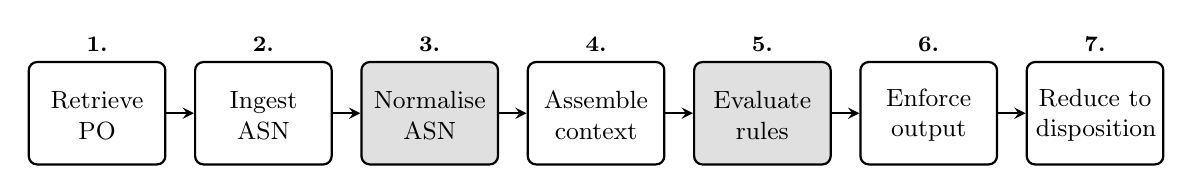
\begin{tikzpicture}[
    node distance=0.35cm,
    stage/.style={
        rectangle, draw=black, thick, rounded corners=3pt,
        minimum width=1.7cm, minimum height=1.3cm,
        text width=1.5cm, align=center, font=\small
    },
    llmstage/.style={
        stage, fill=black!12
    },
    arr/.style={->, thick, >=stealth},
    numlabel/.style={font=\footnotesize\bfseries, above=0pt}
]
% Nodes
\node[stage]    (s1) {\strut Retrieve\\PO};
\node[stage, right=of s1] (s2) {\strut Ingest\\ASN};
\node[llmstage, right=of s2] (s3) {\strut Normalise\\ASN};
\node[stage, right=of s3] (s4) {\strut Assemble\\context};
\node[llmstage, right=of s4] (s5) {\strut Evaluate\\rules};
\node[stage, right=of s5] (s6) {\strut Enforce\\output};
\node[stage, right=of s6] (s7) {\strut Reduce to\\disposition};

% Stage numbers
\node[numlabel] at (s1.north) {1.};
\node[numlabel] at (s2.north) {2.};
\node[numlabel] at (s3.north) {3.};
\node[numlabel] at (s4.north) {4.};
\node[numlabel] at (s5.north) {5.};
\node[numlabel] at (s6.north) {6.};
\node[numlabel] at (s7.north) {7.};

% Arrows
\draw[arr] (s1) -- (s2);
\draw[arr] (s2) -- (s3);
\draw[arr] (s3) -- (s4);
\draw[arr] (s4) -- (s5);
\draw[arr] (s5) -- (s6);
\draw[arr] (s6) -- (s7);


\end{tikzpicture}
}
\caption{Seven stage compound pipeline. Shaded blocks indicate stages that invoke the language model.}
\label{fig:method:pipeline}
\end{figure}



%% -----------------------------------------------------------------
\section{Constraints on the language model's use}
\label{sec:method:constraints}

The pipeline's primary model is the Azure OpenAI gpt-5.4-mini deployment, accessed through the chat completions interface and held fixed across all 5 designs, so that any difference between the designs is attributable to the enforcer and not to the model. To check that the findings are not specific to one model family, the buyer cohort is also run under a second model, Mistral-Large-3 on Azure AI Foundry, with the result reported in Chapter~\ref{chap:results}. A language model raises 2 difficulties that deterministic components do not: the decoder is probabilistic, so the same input can yield different outputs; and a well formed output is not guaranteed to match the structure the next stage expects. Two principles address these.

\emph{Deterministic decoding.} The temperature is set to 0 and the seed fixed, so the decoder selects the highest probability token at each step. This does not make inference strictly deterministic, so every case is processed 5 times under each design and the reported verdict is the majority across the 5 runs; majority voting over repeated samples is a standard stabiliser for sampled decoders \citep{wang2023selfconsistency}. The rate at which the runs agree is reported in Chapter~\ref{chap:results} as a measure of reproducibility.

\emph{Structured outputs.} The output shape is constrained by a schema that declares its fields, their types, and which are required, with the decoder forbidden from producing tokens that would violate it, which removes the need for defensive parsing downstream. Constrained decoding \citep{geng2025} is applied selectively: Stage~3 (ASN normalisation) uses it and gains structural reliability at no cost to reasoning, while Stage~5 (rule evaluation) does not, because format restricting constraints can degrade reasoning on multi step computation \citep{tam2024}. Structural validity of the Stage~5 output is instead recovered post hoc by the enforcer, applying the decoupling principle of \citet{wang2025slot}.

These principles secure the form of the output, its reproducibility and shape, but not its content: a schema valid object from Stage~3 is not guaranteed to carry the values written in the cXML. The methodology assumes Stage~3 normalises the notice faithfully, which is reasonable because the input is machine generated, schema valid cXML rather than free text, and is performed under the deterministic decoding above. The assumption does not threaten the comparison either, since Stages~1 to~4 are shared by all 5 designs, so any normalisation error is constant across them and cancels; Stage~3 is validated empirically in Section~\ref{sec:results:normfidelity} (Table~\ref{tab:results:normfidelity}), which finds 99 per cent field-level fidelity against a deterministic parse. The released code, data, and run artefacts that let every figure and table in Chapter~\ref{chap:results} be regenerated are listed in Appendix~\ref{app:repro}.


%% -----------------------------------------------------------------
\section{Supplier conditioned prompting}
\label{sec:method:supplier}

Stage~4 assembles the validation context that Stage~5 evaluates, and the methodology adapts it to each supplier. The pipeline sees the same suppliers repeatedly and each tends to fail a different subset of the rules, so a supplier that has historically failed a particular rule is more likely to fail it again, a signal the language model has no access to from the cXML alone. The Stage~4 prompt therefore includes a short statement of the supplier's historical validation record before the language model is invoked. The conditioning is dynamic: a case is conditioned only on that supplier's earlier validated cases, so the prior grows as history accumulates and never draws on a future case. A supplier's first case therefore starts from an empty prior, a cold start.

The construct draws on the retrieval augmented generation family of \citet{lewis2020rag}, instantiating 2 of its elements: a non parametric memory of prior cases held outside the model's weights, and a generator prompted, at inference time, on content drawn from that memory. The retrieval is a deterministic lookup on the supplier identifier, so the construct is referred to as supplier conditioned prompting rather than as retrieval augmented generation in full.

Each profile records the dispositions previously assigned to the supplier's notices, the rules they most often failed, and a one sentence summary, and that summary is what the prompt receives. Two inclusion criteria apply: profiles are built only from buyer confirmed cases, never from the pipeline's own output, so the layer cannot learn from and amplify its own mistakes; and a supplier enters the corpus only with at least 2 buyer validated cases, so that leave-one-out evaluation can hold one out without leaving the prior empty. The supplier by supplier breakdown is given in Chapter~\ref{chap:empirical}.

The conditioning's effect is isolated by an ablation with 3 arms: off; on, under a leave-one-out protocol; and a placebo that carries a different supplier's history under the same framing. A strict past-only variant, which conditions each case on the supplier's earlier cases alone, additionally checks that the leave-one-out result does not depend on look-ahead. The ablation looks only at the 14 rules in the language model regime and at the disposition, because the enforcer of Section~\ref{sec:method:enforcer} owns the 8 deterministic regime rules and overrides any verdict the conditioning could move on them; those are the only places where the prior can still register. The results are reported in Chapter~\ref{chap:results}.


%% -----------------------------------------------------------------
\section{Prompt engineering techniques}
\label{sec:method:prompt}

The evaluation stage relies on a language model to assess a structured payload against the rule set, and how the task is presented to the model affects the quality of that assessment. Four prompt engineering techniques are applied, each addressing a distinct source of error.

\emph{Persona prompting} \citep{salewski2024} opens the system message with the role the model is to play, which narrows the priors it draws on and improves adherence to domain conventions and vocabulary.

\emph{Task decomposition} \citep{khot2023,zhou2023} splits the task into sub tasks stated explicitly in the prompt. Here the validation is decomposed into 3: aligning the line items of the 2 documents, a rule by rule evaluation, and a semantic analysis of findings the rule set does not capture. Each sub task is narrower than the whole, which reduces the model's load and exposes the intermediate structure to the consuming stage.

\emph{Few shot prompting} \citep{brown2020} appends a small number of worked examples that demonstrate the desired output format and the conventions for evaluating rules. It is especially effective when the output is structured, since the examples collapse variance in field naming and in explanation granularity.

\emph{Chain of thought prompting} \citep{wei2022} instructs the model to state its intermediate calculations before committing to a verdict. It is applied to R01, R02 and R15, the rules needing tolerance band arithmetic on quantities, unit prices and line totals, where it reduces single step arithmetic errors. It is deliberately not applied to the semantic sub task, because explanations can be unfaithful when the model has no clean verification procedure \citep{turpin2023}.

Examples of each technique as applied in the Stage~5 prompt are reproduced in Appendix~\ref{app:prompt} (Table~\ref{tab:app:prompt}).


%% -----------------------------------------------------------------
\section{The enforcer pattern}
\label{sec:method:enforcer}

The methodological contribution of this dissertation is a design pattern for combining language model evaluation with deterministic verification on a rule by rule basis. The pattern addresses 2 limitations of an unconstrained language model evaluator. The first is that language models are empirically unreliable on closed form arithmetic \citep{arkoudas2023,dziri2024}, whereas a deterministic check provides a reproducible answer. The second is that when a language model sees a contradiction in its input, for example, 2 fields that should match but do not, it tends to produce a smoothed over answer rather than report the conflict \citep{huang2024hallucination}.

In plain terms, the enforcer pattern is built around 2 design decisions, both fixed at design time: which rules are evaluated deterministically rather than by the language model, and when the deterministic check runs relative to the language model: before, during, or after. The remainder of this section formalises this idea, names the 2 regimes (rule ownership), and characterises the 3 realisations (timing).

\subsection{Definition}
\label{sec:method:enforcer:def}

For each rule $r_i$ in the rule set $R = \{r_1, \ldots, r_n\}$, the enforcer produces a final verdict and severity $(v_i, s_i)$ by applying a rule specific function $\varphi_i$. The enforcer is a deterministic Stage~6 component; the language model is invoked only inside Stages~3 and~5. The output of the enforcer is the indexed collection
%
\begin{equation}\label{eq:enforcer}
  E(R) = \{(r_i, v_i, s_i)\}_{i=1}^{n}
\end{equation}
%
of (rule, verdict, severity) triples, one for each of the $n$~rules in $R$, used as input to the disposition reduction in Section~\ref{sec:method:disposition}.

The function has 2 degrees of freedom. The first is \emph{rule ownership}: for rules in the language model regime, $\varphi_i$ accepts the language model's verdict unchanged; for rules in the deterministic regime, $\varphi_i$ is a procedure implemented in code (Section~\ref{sec:method:enforcer:regimes}). The second is \emph{realisation}: the deterministic check may run before, during, or after the language model's evaluation, and the input to $\varphi_i$ follows from this choice (Section~\ref{sec:method:enforcer:realisations}).

To illustrate, suppose the language model emits $(\text{ok},\; \text{info})$ for some rule $r_i$. If $r_i$ belongs to the language model regime, the enforcer leaves the triple unchanged as $(r_i,\; \text{ok},\; \text{info})$. If $r_i$ belongs to the deterministic regime and the deterministic check finds a violation, the enforcer returns $(r_i,\; \text{fail},\; \text{crit})$, overriding the language model's verdict.

\subsection{Two regimes (rule ownership)}
\label{sec:method:enforcer:regimes}

Two regimes are used. In the \emph{language model regime}, $\varphi_i$ is the identity function and the language model's verdict is accepted unchanged. In the \emph{deterministic regime}, $\varphi_i$ is the result of a deterministic check implemented in code, whether that procedure runs before, during, or after the language model.

Rules are assigned by category and by one further test: a rule joins the deterministic regime only if its check reduces to a closed form computation on fields the pipeline already has. Semantic rules cannot meet this test by definition and always sit in the language model regime. Most arithmetic and structural rules can, but not all: R05 (unit of measure equivalence) and R20 (weight plausibility), for example, need their inputs interpreted before the check can run, so they stay in the language model regime. Eight rules pass the test (R01, R02, R03, R06, R15, R16, R18, and R19) and form the deterministic regime; the other 14 are evaluated by the language model.

\subsection{Three realisations (when the deterministic check is applied)}
\label{sec:method:enforcer:realisations}

The deterministic regime admits 3 realisations of $\varphi_i$, differing only in when the deterministic check runs relative to the language model.

The first is \emph{post hoc}. The language model emits a verdict $(\hat{v}_i, \hat{s}_i)$ at Stage~5 for every rule. At Stage~6, each deterministic regime rule is recomputed in code, and $\varphi_i$ takes the language model's prior verdict as input:
%
\begin{equation}\label{eq:posthoc}
  (v_i, s_i) = \varphi_i(\hat{v}_i, \hat{s}_i)
\end{equation}

The second is \emph{in generation}. The deterministic check is exposed through tool calling, a provider side mechanism by which the language model emits a structured call to an external function and receives its return value as additional context before continuing to generate. The language model invokes the tool at Stage~5 before committing to a verdict, and $\varphi_i$ takes the document pair $(p, a)$ directly:
%
\begin{equation}\label{eq:ingen}
  (v_i, s_i) = \varphi_i(p, a)
\end{equation}
%
for each rule $r_i$ in the deterministic regime. The 7 callable tools used in this realisation are enumerated in Appendix~\ref{app:rules} (Table~\ref{tab:method:tools}). One rule, R18 (duplicate detection), cannot be exposed as a tool in this realisation: deciding whether a notice is a duplicate needs memory of earlier notices, which a single stateless tool call does not have, so in Mode~D R18 is settled by a post hoc check instead. R18 is also tested on its own, by submitting the same notice twice together with a fresh one as a control and checking that only the repeat is flagged; the result is reported in Chapter~\ref{chap:results}.

The third is \emph{pre hoc}. The deterministic check runs before the language model is invoked, and its verdicts on the deterministic regime rules are written into the language model's input context. The language model is asked only about the rules in the language model regime and never produces a verdict on the deterministic regime rules. Equation~\eqref{eq:ingen} holds here, with $\varphi_i$ computed before the language model rather than during it.

The 3 realisations encode the same $\varphi_i$ and form a gradient of enforcement strength. In generation enforces the constraint softly: the language model decides how to use the tool result. Post hoc enforces it strictly: the language model's verdict on the deterministic regime rules is replaced at Stage~6. Pre hoc enforces it most strictly: the language model never produces a verdict on the deterministic regime rules and so cannot contradict them. This gradient, soft, strict, strictest, is the methodological pivot of Section~\ref{sec:method:ablation}. Only the 2 strict positions hold deterministic authority over the verdict; the soft in generation realisation is established tool use \citep{schick2024,goodell2025} that leaves the final verdict to the model, and it enters the comparison as the prior art control that isolates the effect of that authority. Figure~\ref{fig:method:realisations} summarises the 3 realisations and their temporal relationship to the language model.

\begin{figure}[htbp]
\centering
% Three realisations of the enforcer pattern
% Requires: \usepackage{tikz}, \usetikzlibrary{positioning, arrows.meta, calc}
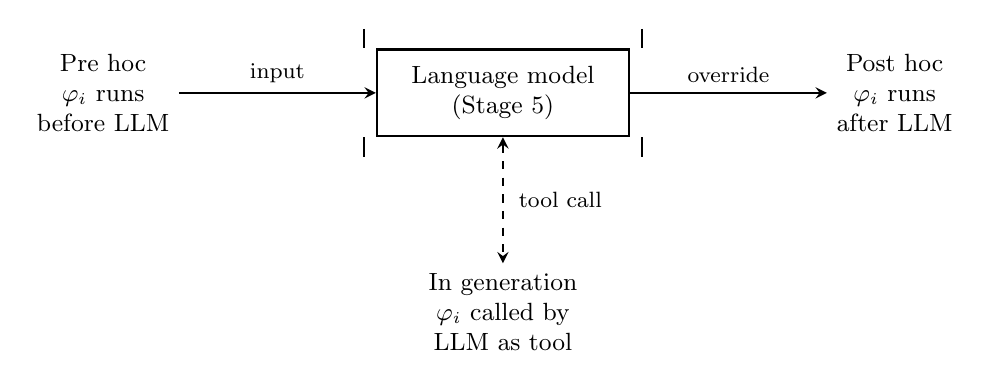
\begin{tikzpicture}[
    node distance=0.8cm and 1.8cm,
    box/.style={
        rectangle, draw=black, thick,
        minimum width=3.2cm, minimum height=1.1cm,
        align=center, font=\small
    },
    label/.style={
        align=center, font=\small
    },
    arr/.style={->, thick, >=stealth},
    darr/.style={<->, thick, >=stealth, dashed},
]

% Central box: Language model (Stage 5)
\node[box] (llm) {Language model\\(Stage~5)};

% Pre-hoc (left)
\node[label, left=2.5cm of llm] (pre) {Pre hoc\\$\varphi_i$ runs\\before LLM};

% Post-hoc (right)
\node[label, right=2.5cm of llm] (post) {Post hoc\\$\varphi_i$ runs\\after LLM};

% In-generation (below)
\node[label, below=1.6cm of llm] (ingen) {In generation\\$\varphi_i$ called by\\LLM as tool};

% Connecting lines
% Pre-hoc: arrow from pre to the left side of LLM
\draw[arr] (pre.east) -- (llm.west)
    node[midway, above, font=\footnotesize] {input};

% Post-hoc: arrow from right side of LLM to post
\draw[arr] (llm.east) -- (post.west)
    node[midway, above, font=\footnotesize] {override};

% In-generation: bidirectional dashed arrow from LLM bottom to ingen
\draw[darr] (llm.south) -- (ingen.north)
    node[midway, right, font=\footnotesize, xshift=2pt] {tool call};

% Brackets connecting pre-hoc to LLM input
\draw[thick] ($(llm.north west)+(-0.15,0.25)$) -- ($(llm.north west)+(-0.15,0)$);
\draw[thick] ($(llm.south west)+(-0.15,-0.25)$) -- ($(llm.south west)+(-0.15,0)$);

% Brackets connecting LLM output to post-hoc
\draw[thick] ($(llm.north east)+(0.15,0.25)$) -- ($(llm.north east)+(0.15,0)$);
\draw[thick] ($(llm.south east)+(0.15,-0.25)$) -- ($(llm.south east)+(0.15,0)$);

\end{tikzpicture}

\caption{Three realisations of the enforcer pattern, by when the deterministic check $\varphi_i$ runs relative to the language model: before (pre hoc), during (in generation), or after (post hoc).}
\label{fig:method:realisations}
\end{figure}

\subsection{Auxiliary operations: rule injection and severity capping}
\label{sec:method:enforcer:aux}

The enforcer also performs 2 operations that lie outside the override function definition. The first is \emph{rule injection}: if the language model omits a rule's verdict, the enforcer inserts one, which is recomputed deterministically for rules in the deterministic regime, or set to a default with a diagnostic note for rules in the language model regime. The second is \emph{severity capping}: each rule has a defined severity in the rule register (Appendix~\ref{app:rules}, Table~\ref{tab:app:rules}); if the language model assigns a severity that differs from the rule's registered value, the enforcer clamps it to the registered value. Both operations are expressed as structured actions and are written into the run artefact.

Both operations apply in every realisation of the enforcer pattern (post hoc, in generation, pre hoc). In the pre hoc realisation, both operate only on the language model regime, since the deterministic regime verdicts were finalised at Stage~5.

Every modification the enforcer makes to a triple is recorded in the run artefact as one of 3 logged action types: the override of Section~\ref{sec:method:enforcer:def} and the 2 auxiliary operations introduced above. They are listed in Appendix~\ref{app:rules} (Table~\ref{tab:method:actions}). Two rules have severities that are themselves conditional. R16 (partial shipment handling) is registered as informational but its deterministic check escalates it to warning when R01 detects an under shipment against the purchase order baseline. R06 (line item completeness) is registered as critical but its check grades the missing lines as warning when they trace to a declared partial delivery. Both are part of each rule's own logic, not generic enforcer operations, so neither is a separate action type.

The enforcer pattern has 3 parts: a rule ownership assignment, a family of rule specific override functions with 3 realisations, and a small set of auxiliary operations. Whichever realisation is used, the enforcer's output has the same shape, one (rule, verdict, severity) triple per rule plus an action log, so the rest of the pipeline does not depend on which realisation produced the verdict.


%% -----------------------------------------------------------------
\section{Disposition reduction}
\label{sec:method:disposition}

The final stage reduces the enforcer's output $E(R)$ of Equation~\eqref{eq:enforcer} to a single disposition by applying a deterministic rule. Let $c$ be the number of failed rules with critical severity, and $w$ the number with warning severity. The disposition is defined by
%
\begin{equation}\label{eq:disposition}
  \text{disp}(E(R)) =
  \begin{cases}
    \textsc{reject} & \text{if } c \geq 1, \\
    \textsc{review} & \text{if } c = 0 \;\wedge\; w \geq 1, \\
    \textsc{pass}   & \text{if } c = 0 \;\wedge\; w = 0.
  \end{cases}
\end{equation}

The policy is deliberately conservative: one critical failure forces rejection and one warning forces review, because a false acceptance costs far more than a false review. Informational findings do not enter the reduction.


%% -----------------------------------------------------------------
\section{Ablation design}
\label{sec:method:ablation}

To isolate the contribution of the enforcer, the pipeline is evaluated under 5 alternative designs. The designs vary the role of the deterministic regime: whether it is used, where in the pipeline it is applied, and whether it is replaced by a neural auditor. The set of designs is given in Table~\ref{tab:method:ablation}.

\begin{table}[htbp]
\centering
\caption{Ablation design.}
\label{tab:method:ablation}
\footnotesize
\begin{adjustbox}{max width=\textwidth}
\begin{tabular}{@{}cp{3.8cm}p{3.8cm}p{3.6cm}p{2.2cm}@{}}
\toprule
\textbf{Mode} & \textbf{Stage~5} & \textbf{Stage~6} & \textbf{Det.\ rules} & \textbf{Role} \\
\midrule
A: none          & LLM, all rules                                    & Pass through                              & ---                                          & Baseline              \\[6pt]
B: post hoc      & LLM, all rules                                    & Deterministic check on the 8~owned rules  & R01, R02, R03, R06, R15, R16, R18, R19       & Post hoc override     \\[6pt]
C: LLM-as-judge  & LLM, all rules                                    & Second LLM auditor, all rules             & ---                                          & LLM-as-judge          \\[6pt]
D: in generation & LLM with the 7~tools of Table~\ref{tab:method:tools}, all rules & Pass-through, with R18 fallback  & R01, R02, R03, R06, R15, R16, R19; R18       & In generation tool use \\[6pt]
E: pre hoc       & Det.\ check on 8~owned rules; LLM on remaining~14 & Merge; severity capping and injection on LM-regime verdicts & R01, R02, R03, R06, R15, R16, R18, R19 & Pre hoc split \\
\bottomrule
\end{tabular}
\end{adjustbox}
\end{table}

The 5 designs, labelled Mode~A to Mode~E, are the 3 realisations of the enforcer pattern (post hoc, in generation, pre hoc) and 2 designs outside it. Mode~A is an unprocessed baseline: the language model evaluates every rule and nothing post-processes it, which isolates the evaluation stage on its own. Mode~C (LLM-as-judge) replaces the deterministic check with a language model call at Stage~6, testing whether a neural auditor can stand in for a deterministic one. Mode~B overrides the model's verdicts afterwards (post hoc), Mode~D exposes the checks as tools the model calls during generation (in generation), and Mode~E runs them first and asks the model only about the remaining 14 rules (pre hoc). R18, which needs cross-document state,  is always settled by the deterministic side.

The designs serve 2 comparisons. The full 5 way comparison answers RQ.1, on how the designs compare on per rule accuracy, disposition, cost and latency. The 3 way contrast among B, D and E answers RQ.2 by isolating the enforcer's position while holding rule scope and logic fixed; Mode~A bounds the comparison from below, and Mode~C contributes to RQ.1 only. RQ.3 is answered separately, by the supplier conditioning ablation below, which is orthogonal to the 5 designs.

That ablation is the one defined in Section~\ref{sec:method:supplier}. Comparing off with on shows whether the prior helps; comparing on with placebo shows whether any gain comes from the specific history or merely from an authoritative looking sentence. The effect is clearest in Mode~A, where no enforcer override can mask it, and the results are reported with the 5-design comparison in Chapter~\ref{chap:results}.


%% -----------------------------------------------------------------
\section{Evaluation instrument}
\label{sec:method:eval}

The evaluation compares the pipeline's output against a reference produced by a human expert. Four outcomes are measured, matching the 4 targets of RQ.1 and RQ.2: agreement on the document level disposition, accuracy on each individual rule, cost, and latency.

For the document level disposition, the primary metric is Cohen's quadratically weighted kappa \citep{cohen1968kappa}. The disposition has 3 ordered values (\textsc{pass}, \textsc{review}, \textsc{reject}), and the quadratic weighting penalises a far disagreement more than a near one, so a pass to reject error weighs 4 times a pass to review or review to reject error. The coefficient is 1 at perfect agreement and 0 at chance; its definition is given in Appendix~\ref{app:metrics}.

Cohen's kappa can drop sharply when one disposition value dominates the dataset, even when agreement is in fact high \citep{cicchetti1990}. The evaluation therefore also reports Gwet's AC2 \citep{gwet2008}, which has the same chance corrected form but a chance agreement term less sensitive to category imbalance. The 2 are reported side by side, and a divergence between them signals that prevalence is distorting the kappa. A $3 \times 3$ confusion matrix per design shows the structure of the agreement, since 2 designs with the same $\kappa_w$ can have very different error patterns.

For per rule accuracy, each rule's pipeline verdict is compared against the expert's verdict for the same rule on the same document, with precision and recall reported per rule treating \emph{fail} as the positive class. These are summarised by a severity weighted macro F1, which weights each rule's F1 by its registered severity (1~informational, 2~warning, 3~critical) so that higher consequence rules count for more; its definition is in Appendix~\ref{app:metrics}.

Cost is reported as the average number of input and output tokens consumed per document, with the conversion to currency given in Chapter~\ref{chap:results}. Latency is reported as the average wall clock time per document, in seconds. Both are reported as means with standard deviations, computed across the 5 repeated runs defined in Section~\ref{sec:method:constraints}.


When the 5 designs are compared in Chapter~\ref{chap:results}, each point estimate is read together with its confidence interval. The bootstrap intervals are 95\% percentile intervals from 2,000 resamples, used because the samples are small. For the same reason the comparison is primarily descriptive: most differences are judged on their direction and size, their confidence intervals, and how stable the verdicts are across repeated runs, rather than on significance alone. Where a contrast is large enough to be statistically reliable, it is reported as such.

Three paired tests support this reading. Each pair of designs is compared with an exact McNemar test \citep{dietterich1998approximate} on whether each case is right or wrong, the exact form being used because the counts are too small for the usual approximation; a Holm correction \citep{holm1979simple} is applied across each family of comparisons; and Cohen's h \citep{cohen1988statistical} gives a rough effect size. The tests are supporting evidence, not pass/fail decisions: a non-significant result is reported as such, and effect sizes with intervals are preferred over significance stars \citep{berrar2017confidence}. Both the bootstrap and the McNemar test assume the cases are independent, which holds only partly on the buyer sample, a point Chapter~\ref{chap:results} returns to.

The supplier conditioning ablation is read on the same instrument. Within each mode, its off, on, and placebo settings are compared on the disposition agreement coefficients ($\kappa_w$ and AC2) and on a severity weighted macro F1 limited to the 14 language model regime rules, the only rules the prior can move. Changes in disposition are also reported as a paired flip count against the no-conditioning baseline, each flip marked as moving towards or away from the buyer ground truth. Given the small buyer sample, these differences are read through the point estimates, the confidence intervals, and the flip table rather than significance tests, and a difference of zero is reported as such.


%% -----------------------------------------------------------------
\section{Chapter conclusion}

This chapter set out the methodology. The work is framed as design science research in the improvement quadrant. The validation task is formalised as a function from a purchase order and a shipping notice to a disposition, decomposed through a rule set organised by a taxonomy of failure modes, and realised by a 7 stage pipeline, 2 stages of which call a language model. Two principles govern that model, deterministic decoding and structured outputs, and 4 prompt engineering techniques shape the evaluation prompt. The Stage~4 prompt is conditioned on a short, dynamic record of the supplier's prior validations, a lightweight form of retrieval augmented generation.

The core contribution is the enforcer pattern: a rule level scheme that assigns each rule to the language model regime or the deterministic regime, with 3 realisations (post hoc, in generation, pre hoc) that share the same rule ownership and differ only in when the deterministic check runs. Its effect is isolated by an ablation of 5 designs, 3 that instantiate the pattern and 2 outside it, and the supplier conditioning by a second, orthogonal ablation. Disposition agreement (weighted kappa and Gwet's AC2), severity weighted per rule F1, cost and latency are the measures, read descriptively with bootstrap confidence intervals. The next chapter applies this methodology.
%% =====================================================================
%%  4_empirical_study.tex --- Chapter 4: Empirical Study
%% =====================================================================

\chapter{Empirical Study} \label{chap:empirical}

This chapter situates the artefact of Chapter~\ref{chap:method} in its industrial context and assembles the empirical material on which Chapter~\ref{chap:results} reports. It opens with a short profile of the partner organisation, walks the AS-IS process and the 8 pain points it surfaces, and sketches the TO-BE artefact that follows from those pain points. The bulk of the chapter then specifies the evaluation design: the data sources, the 3 block composition of the evaluation set, the supplier level failure clustering, the per-case ground truth on the buyer sample, the synthetic perturbation matrix and the ground truth construction protocol. The chapter's contribution is twofold: it specifies the case in which the artefact is evaluated, with explicit operational measures, and it constructs an evaluation set under which the next chapter's results are interpreted.


%% -----------------------------------------------------------------
\section{Introduction}
\label{sec:emp:intro}

This chapter operationalises the Chapter~\ref{chap:method} methodology against a real procurement case at Hilti AG. The case scope is fixed throughout: the Procurement function inside Hilti's Sourcing, Innovation and Competence Division; the commerce eXtensible Markup Language (cXML) Advanced Shipping Notice (ASN) as the validated document; and the rule register introduced in Section~\ref{sec:method:taxonomy}.


%% -----------------------------------------------------------------
\section{Case organisation: Hilti and the procurement function}
\label{sec:emp:case}

The empirical work reported here is conducted inside Hilti AG, a Liechtenstein headquartered manufacturer of professional construction, fastening and measuring equipment, with a 2025 global turnover of CHF 6.3~bn, around 34{,}400 employees and a direct sales footprint in more than 120 countries.\footnote{Company figures from Hilti Group public reporting.} Specifically, the work is conducted inside the Sourcing, Innovation and Competence Division, where a Procurement department is responsible for the source-to-pay transactions that govern incoming goods from external suppliers. The case is methodologically informative in 3 respects: a defined gate at which the artefact intervenes (the partner’s enterprise system), a documented operational process and a buyer validated pain-point inventory (Section~\ref{sec:emp:asis}), and a heterogeneous supplier profiles base across different integration modes, against which the artefact's supplier conditioned layer can be exercised. Following the case study guidance of \citet{yin2018case} and \citet{runeson2009}, this study treats the case as suited to single case industrial study on 3 grounds: a clearly defined unit of analysis, a stable operational context, and a researcher accessible site that permits both archival data extraction and stakeholder interviews.

The Advanced Shipping Notice (ASN) is at the centre of the case. An ASN is the cXML document that a supplier transmits to Hilti, through the procurement platform's electronic data interchange (EDI) channel, to declare the contents and the dispatch parameters of an outbound shipment against a previously issued Purchase Order (PO). On receipt, the ASN is matched against the PO baseline by the partner's enterprise system; a mismatch, whether in quantity, unit of measure, currency, delivery date or any of numerous further attributes, blocks the goods receipt, and the buyer is drawn into a manual reconciliation loop that involves reading the cXML by hand and emailing the supplier.


Table~\ref{tab:emp:asis_baseline} consolidates the operational baseline of the AS-IS process. The volume figures describe the function; the per-defect handling time and the time to resolution are reported by the buyer team, drawn from interviews with 3 analysts and past ASN resolution logs. Production ASN defects are usually cleared in a single iteration, whereas pre-integration cases run longer because they involve repeated back-and-forth with the supplier. The annual cost projection that scales these figures, with its assumptions, is derived in Appendix~\ref{app:operational}.

\begin{table}[htbp]
\centering
\caption{AS-IS operational baseline.}
\label{tab:emp:asis_baseline}
\small
\begin{tabular}{@{}lp{7.5cm}@{}}
\toprule
\textbf{Metric} & \textbf{Value} \\
\midrule
Live function volume & Of the order of 28,000 ASNs per year \\
Manual handling per defect          & 30 to 90 minutes (buyer reported) \\
Time to resolution, production      & 2 to 5 days, usually a single iteration\\
Time to resolution, pre-integration & About 2 months on average (9 cases sampled from past resolution email threads, ranging from days to roughly 5 months)\\
\bottomrule
\end{tabular}
\end{table}


%% -----------------------------------------------------------------
\section{The AS-IS process and its pain points}
\label{sec:emp:asis}

The AS-IS ASN validation process is a swimlane covering 4 actors: the Hilti buyer, the partner's system, the supplier, and the communication channel; the swimlane is shown in Figure~\ref{fig:emp:asis}, and is reproduced with the pain point markers annotated in Appendix~\ref{app:emp:asis} (Figure~\ref{fig:app:asis}). The process unfolds in 5 phases. Phase~1 (PO Creation) is internal to Hilti. Phase~2 (ASN Submission) is the supplier transmitting the cXML to the partner system. Phase~3 (Decision) is binary: the partner system either accepts the ASN or rejects it without further triage. Phase~4 is the manual remediation loop: the buyer checks the errors flagged by the partner system, fixes the ASN by hand, and exchanges emails with the supplier until both sides agree on a corrected version. Phase~5 closes the case with the Transport Advice creation.

\begin{figure}[htbp]
\centering
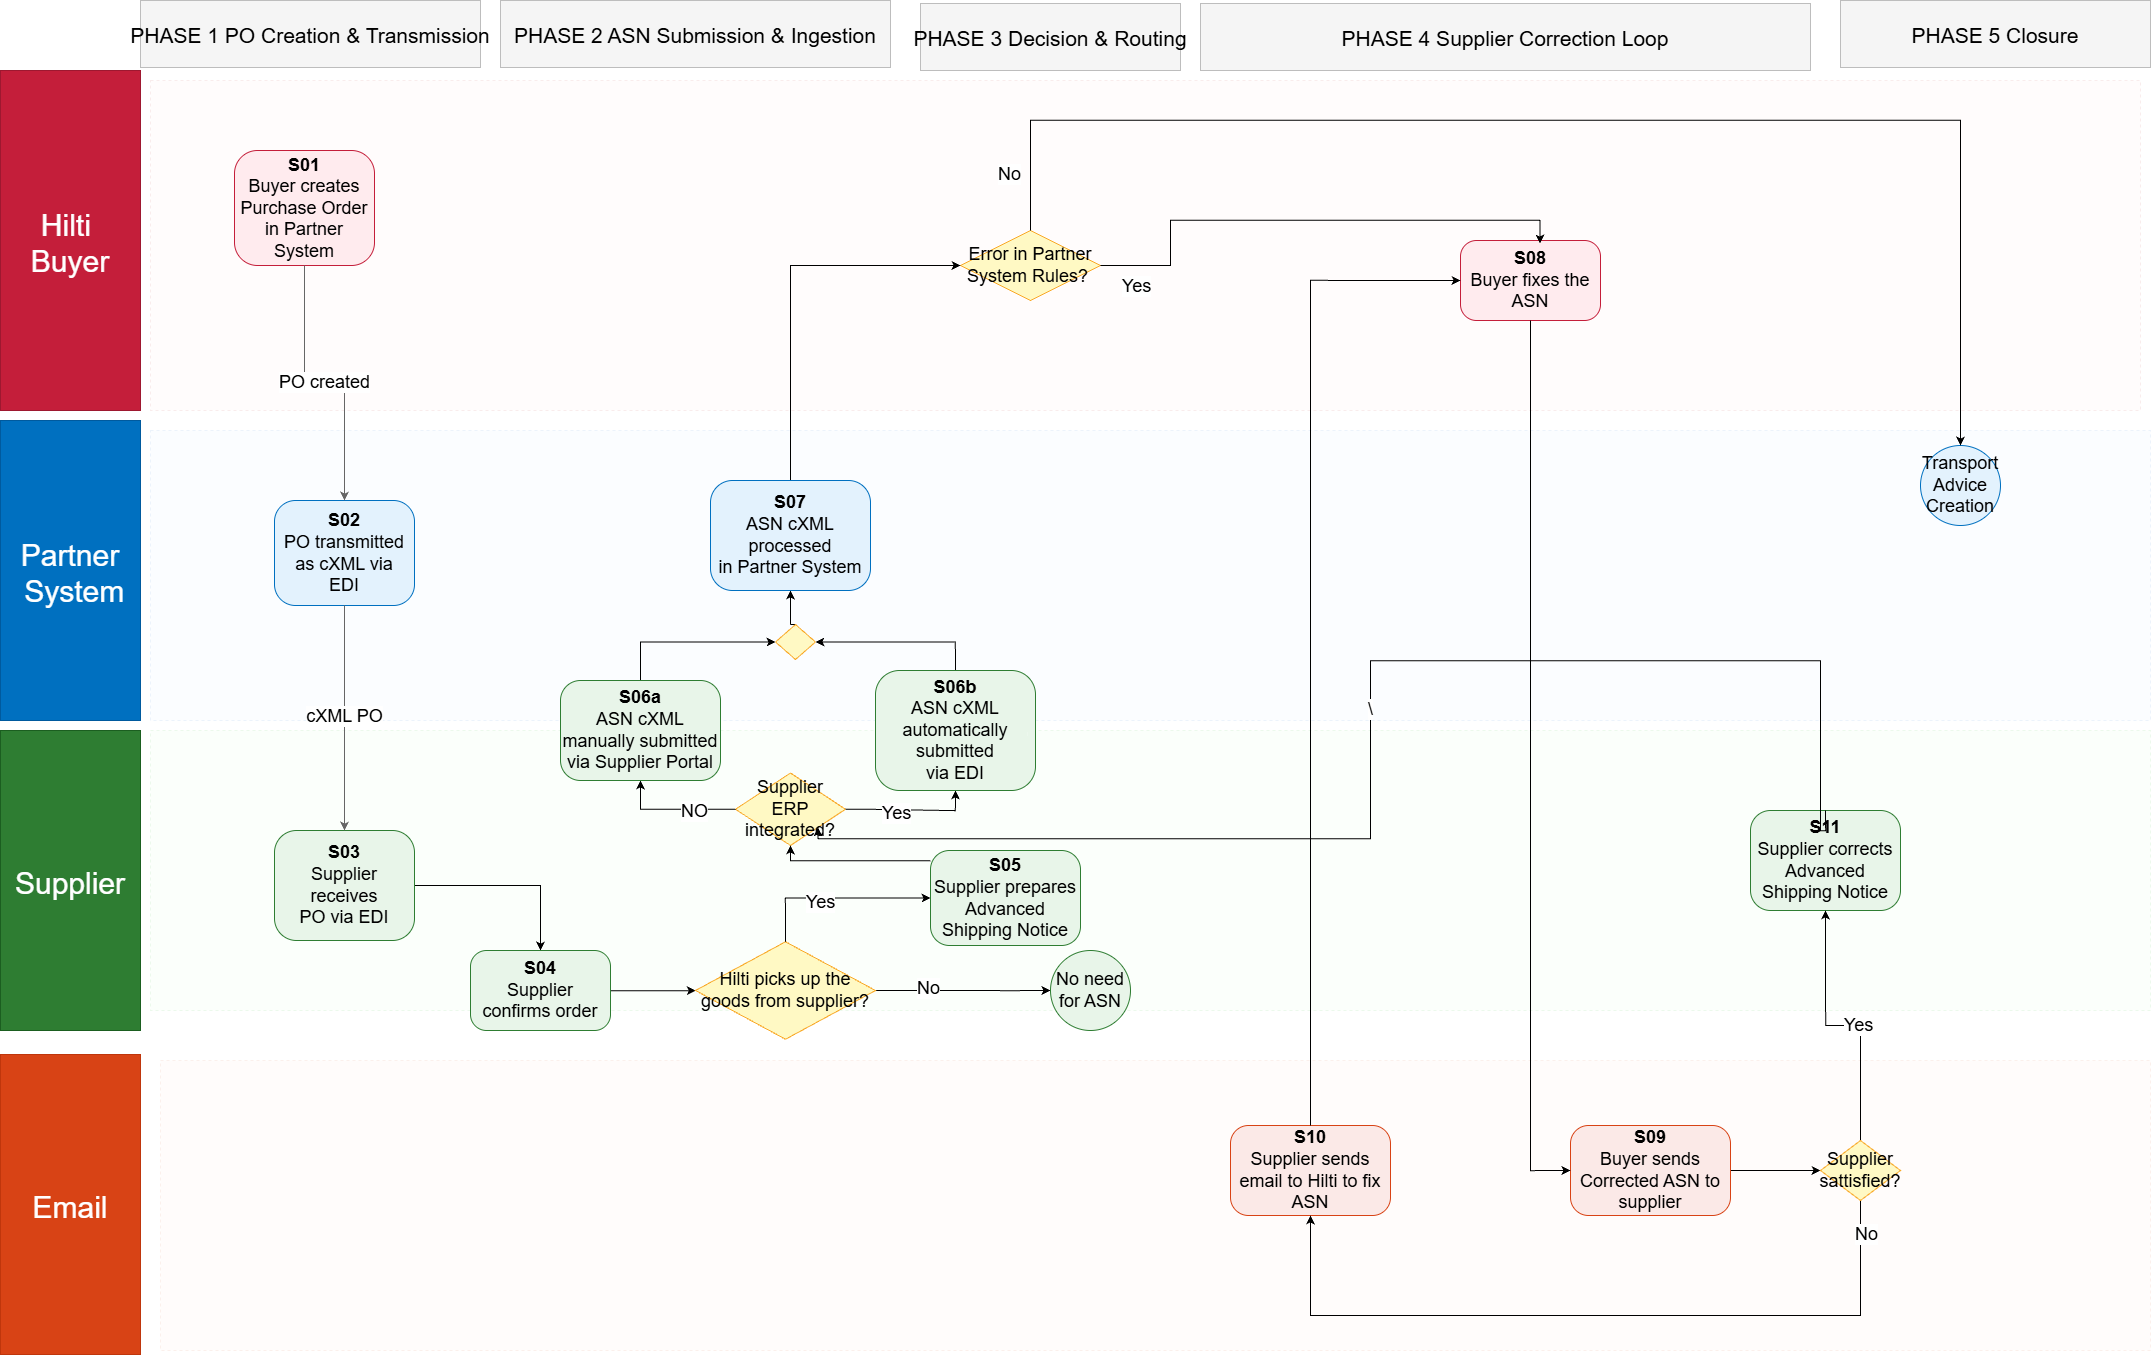
\includegraphics[width=\textwidth]{Figures/fig_4_1_asis_swimlane.pdf.png}
\caption{AS-IS PO--ASN validation process.}
\label{fig:emp:asis}
\end{figure}

The pain point annotation was produced jointly with the buyer team. The 8 pain points it surfaces are reproduced in Table~\ref{tab:emp:painpoints}, with severity assigned by the buyer team on a 3 level scale (Critical, High, Medium) and a root cause attached to each.

\begin{table}[htbp]
\centering
\caption{AS-IS pain points, with severity and root cause.}
\label{tab:emp:painpoints}
\footnotesize
\begin{adjustbox}{max width=\textwidth}
\begin{tabular}{@{}llp{1.6cm}p{9.5cm}@{}}
\toprule
\textbf{\#} & \textbf{Pain point} & \textbf{Severity} & \textbf{Root cause} \\
\midrule
P1 & No automated content validation & Critical & Static field checks only; no semantic, cross-document or supplier history validation, and some defects fail silently. \\
P2 & Manual correction loop & Critical & Buyers interpret each ASN error by hand, email the supplier, and iterate until a corrected version is agreed; the per-defect time and round trip latency are buyer reported rather than measured in this study. \\
P3 & Manual portal entry & High & Light account suppliers type ASNs by hand into the procurement portal, producing typographic and unit of measure errors. \\
P4 & Faulty ERP integration mapping & High & Misconfigured cXML-to-ERP mappings produce the same defect on every ASN from a specific supplier. \\
P5 & No tracking visibility & High & No central tracker; buyers cannot see which ASNs are pending, stuck or escalated. \\
P6 & No supplier history & Medium & Recurring defects are not retained per supplier; the same mistakes recur until solved. \\
P7 & Binary disposition & High & Only accept or reject; no review state for minor or recoverable discrepancies, for example, a late delivery (R03) is rejected on the same gate as a wrong currency (R08), despite the first being recoverable in negotiation. \\
P8 & No audit trail & Medium & Corrections scattered across email; no structured log of why each ASN was accepted or rejected. \\
\bottomrule
\end{tabular}
\end{adjustbox}
\end{table}

For P1, the partner system applies only schema validation and a closed list of static field checks at receipt; it performs no semantic or cross-document check, and some of those checks fail silently, dropping the ASN without an error to the buyer. The full mapping of what the static checks cover, rule by rule, is in Appendix~\ref{app:emp:coverage}.

The 8 pain points fall into 3 classes: upstream, processing and audit. The artefact does not address all 8; it prioritises by severity and targets. The upstream class (P1, P4) is met by the content validation pipeline, which runs the full rule register on every ASN. The processing class (P2, P7) is met by the tiered disposition layer, which adds a REVIEW state between accept and reject, a design informed by the broader human-in-the-loop principles of \citet{amershi2019}. The audit class (P6, P8) is met by the supplier conditioned prompting layer of Section~\ref{sec:method:supplier} and by a structured audit log of every input, prediction and disposition. P3 (manual portal entry) is organisational, not technical, and is out of scope by design; P5 (tracking visibility) is left to future work.

These 3 classes recur in Section~\ref{sec:emp:groundtruth} when the rule level evidence is read against the partner's static check coverage.


%% -----------------------------------------------------------------
\section{The TO-BE artefact}
\label{sec:emp:tobe}

The TO-BE swimlane is shown in Appendix~\ref{app:emp:asis} (Figure~\ref{fig:emp:tobe}). The TO-BE adds 3 new actors to the AS-IS picture: a cloud host that runs the deterministic parser, the prompt builder and the enforcer; a language model service that normalises the cXML payload and assesses each rule against the PO baseline; and a SharePoint log that persists every input, every prediction and every disposition, addressing P8.

The pipeline progresses through 6 phases. Phase~1 (PO Creation and Transmission) is unchanged from the AS-IS. Phase~2 (ASN Submission and Ingestion) captures each cXML envelope into the inbound records; the partner system's existing static checks still fire here but are now one input among many rather than the gatekeeper. Phase~3 (AI Processing) is the new core and realises stages 2 to 6 of the Section~\ref{sec:method:pipeline} pipeline: the deterministic parser ingests the cXML, the language model normalises it into structured JSON, the prompt builder assembles the rule register R01--R22, the PO baseline and the supplier history of Section~\ref{sec:emp:clustering} into a single prompt, the language model assesses each rule and emits a per rule verdict with severity and evidence, and the enforcer reduces those verdicts to a master report. Phase~4 (Decision and Routing) collapses the master report to one of 3 dispositions: PASS, REVIEW or REJECT; addressing pain point P7; REVIEW cases are routed to the buyer for adjudication, REJECT cases trigger an auto-generated correction request that is sent only with the buyer's sanction; the pipeline never communicates with the supplier without a buyer in the loop. Phase~5 (Supplier Correction Loop) closes the case once the buyer has dispatched the discrepancy list and the resubmitted ASN triggers the Transport Advice creation (Phase~6, Closure) that ends the original workflow.

The artefact is therefore human-in-the-loop by design rather than as a fallback, a positioning that builds on the human-in-the-loop work of \citet{amershi2019} and \citet{bansal2021}. The buyer's role shifts from the AS-IS pattern of full manual reconciliation to a review pattern in which the pipeline produces the per rule verdicts, the rationale and the draft correspondence, and the buyer adjudicates REVIEW cases, sanctions REJECT requests before dispatch, and handles the edge cases the pipeline cannot decide. The audit log records the buyer's overrides alongside the pipeline's verdicts, providing a structured source of disagreement data that can inform subsequent revisions to the prompt template and the rule register. The supplier conditioning layer of Section~\ref{sec:method:supplier} draws on the same source: each supplier's prior failure record is built from the audit log entries the buyer has validated, so the history the model reads is grounded in confirmed dispositions and is refreshed as the buyer reviews new cases.

The pipeline is evaluated under the 5 designs specified in Section~\ref{sec:method:ablation} (pure LLM, post hoc, LLM-as-judge, in generation and pre hoc), and the validation logic is the 7 stage compound pipeline of Section~\ref{sec:method:pipeline}. The TO-BE adds the cloud host, the language model service and the SharePoint log, but the stage sequence is unchanged.


%% -----------------------------------------------------------------
\section{Evaluation design}
\label{sec:emp:eval}

This section specifies the conditions under which Chapter~\ref{chap:results} evaluates the artefact: where the data come from and how the evaluation set is composed across 3 blocks (Section~\ref{sec:emp:sources}), which protocol produced the buyer labels (Section~\ref{sec:emp:protocol}), how supplier level failures cluster in the prior corpus that feeds the supplier conditioned prompting layer (Section~\ref{sec:emp:clustering}), what the buyer validated ground truth on the buyer sample looks like (Section~\ref{sec:emp:groundtruth}) and how the synthetic perturbation matrix completes per rule coverage (Section~\ref{sec:emp:synthetic}).


%% -----------------------------------------------------------------
\subsection{Data sources and inclusion}
\label{sec:emp:sources}

The evaluation admits 3 sources: the production stream, the pre-integration stream and a synthetic set; no other source is admitted. A case enters the evaluation set only when

(i)~the source system holds its cXML, guarding the completeness of the document of record,

(ii)~the matching purchase order is also in the source system, guarding referential integrity against the order baseline, and

(iii)~its disposition has been buyer validated or is known by construction, guarding ground truth provenance.

The evaluation set is the residue of a 3 stage filter that implements the inclusion rule (Figure~\ref{fig:emp:filter}) and it contains 100~ASNs across 3 blocks by source: production (Block~A, 28~ASNs), pre-integration (Block~B, 4~ASNs) and synthetic (Block~C, 68~ASNs). The synthetic block carries dispositions known by construction. One case, S-18 (duplicate detection, rule R18), is checked by re-submission rather than a static edit, so 67 of the 68 are evaluable as static dispositions. The production and pre-integration blocks carry the buyer validated dispositions of Section~\ref{sec:emp:protocol}. The full block summary, with each block's source, case range, structural shape and disposition mix, is in Appendix~\ref{app:emp:supporting} (Table~\ref{tab:emp:blocks}).

\begin{figure}[htbp]
\centering
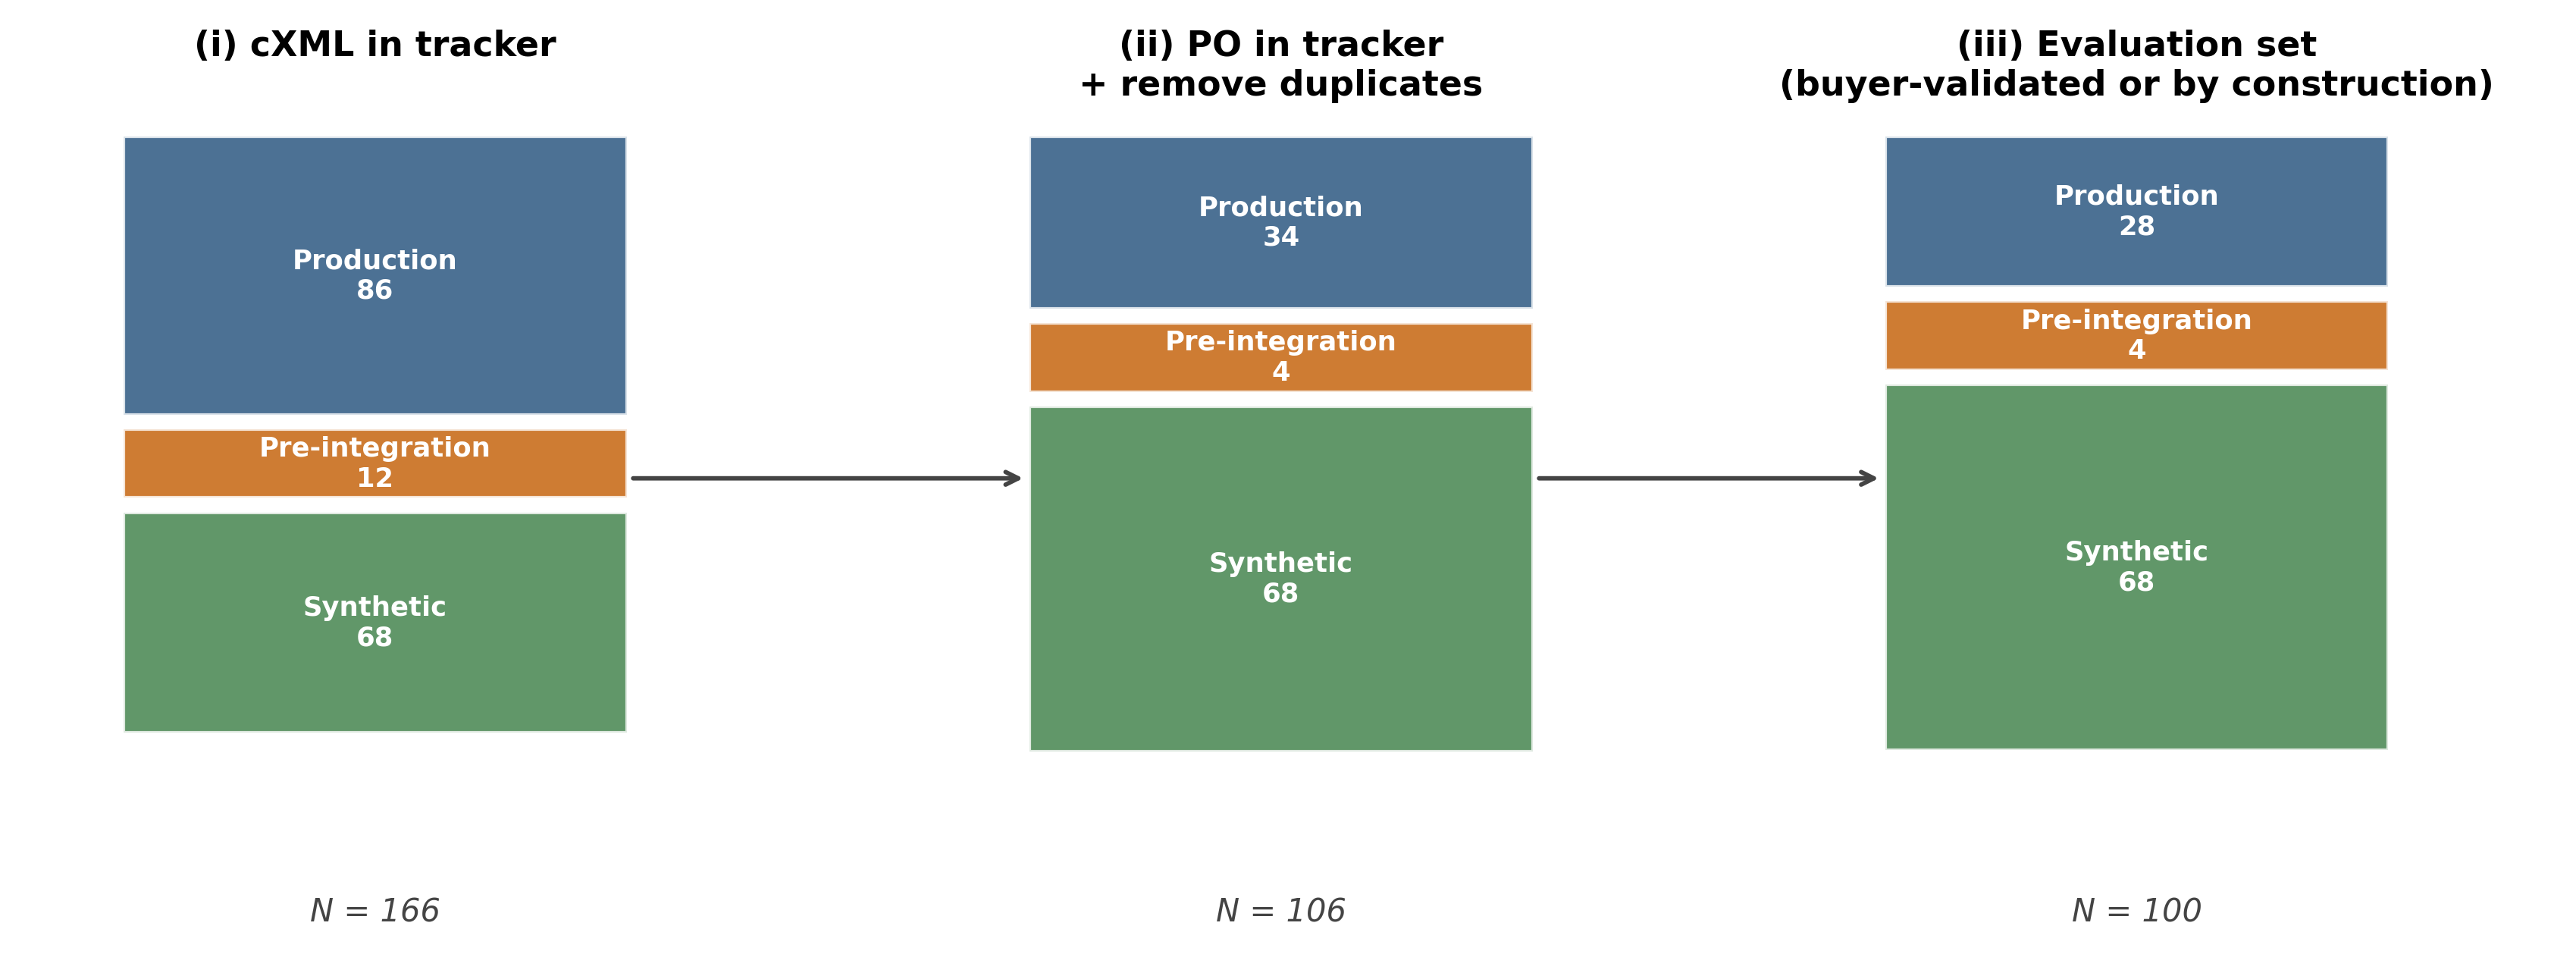
\includegraphics[width=\textwidth]{Figures/fig_4_6_dataset_flow.png}
\caption{Dataset assembly funnel from the raw scrape to the 100-case evaluation set.}
\label{fig:emp:filter}
\end{figure}

\paragraph{Production stream.} The production stream is extracted from the partner's platform tracker, which logs delivery and notification events for source-to-pay traffic. Both rejected and accepted ASNs are eligible, provided the cXML and the matching purchase order are still in the tracker, so the block deliberately mixes the two; the split is reported in Section~\ref{sec:emp:groundtruth}.

\paragraph{Pre-integration stream.} The pre-integration stream comes from the same tracker but covers supplier onboarding, where document exchange with a new supplier is tested before live traffic begins; these cases were curated by the buyer team in a dedicated session. Both real world streams share one constraint: the tracker retains only the last 30 days, which caps how many cases any single scrape yields.

\paragraph{Synthetic perturbation.} The real world cases are too few to exercise every rule individually, so synthetic cases close the gap. Each is a clean production ASN altered by deliberate edits to the cXML, generated deterministically from schema anchored templates rather than by a language model. The block holds 51 single rule mutants (S-01 to S-51) and 17 multi-rule scenarios (SYN-M01 to SYN-M17); their design, and the expected dispositions that follow directly from the edits, are detailed in Section~\ref{sec:emp:synthetic}, so no buyer review is needed.


%% -----------------------------------------------------------------
\subsection{Ground truth construction protocol}
\label{sec:emp:protocol}

The labelling protocol described below was defined in collaboration with the same buyer team that produced the AS-IS swimlane and the pain-point table of Section~\ref{sec:emp:asis}, and applies to every real world ASN that enters the evaluation set. The protocol is deliberately blind: the analysts do not see the pipeline's prediction, and the cases are interleaved on the worksheet by source rather than by the pipeline's verdict, so the analysts are not nudged towards a disposition.

The buyer ground truth is a consensus of 3 procurement analysts. Each labelled every case independently under the blind protocol, and the verdicts were reconciled: agreements stood, and disagreements were adjudicated in a short joint review to a single agreed disposition and rule list. To stay within the analysts' limited availability only this consensus was retained, so an inter-rater coefficient cannot be computed retrospectively. A consensus of several experts is taken here as a stronger reference than a single annotator, drawing on the multi-annotator agreement literature of \citet{artstein2008} and \citet{fleiss1971}. Each label also carries a 5 point analyst confidence, reported in Section~\ref{sec:emp:groundtruth}. The panel is small and shares the partner organisation's conventions, so the reference reflects one organisation's reading of the rules; recording the per analyst labels and widening the panel is part of the deferred validation discussed in Chapter~\ref{chap:results}.

The checklist, the 2 rules pre-filled N/A, and the annotation interface are described in Appendix~\ref{app:emp:annotation}.


%% -----------------------------------------------------------------
\subsection{Failure clustering by supplier}
\label{sec:emp:clustering}

The pipeline (Section~\ref{sec:method:supplier}) feeds the language model a short history of each supplier's past failures, taken from the evaluation set itself. Of the 19 distinct suppliers in the evaluation set, 5 have at least 2 buyer validated cases; the other 14 contribute no history and stay in the evaluation set only as cases.

\begin{table}[htbp]
\centering
\caption{Supplier prior corpus, grouped by failure archetype.}
\label{tab:emp:suppliers}
\footnotesize
\begin{adjustbox}{max width=\textwidth}
\begin{tabular}{@{}lllll p{6cm}@{}}
\toprule
\textbf{Archetype} & \textbf{Supplier} & \textbf{Country} & \textbf{n} & \textbf{Disposition mix} & \textbf{Notes} \\
\midrule
Strongest historical signal       & S1  & AT & 9 & 9 REJECT  & Recurring transport, address, packaging, mandatory field and unit price defects \\
Recurring buyer flagged defects   & S2  & CH & 2 & 2 REJECT  & Unit price and currency mismatch with transport/address drift \\
Upstream bug false positives      & S3  & CH & 3 & 3 PASS    & Timezone issue; content clean \\
Upstream bug with packaging gap   & S4  & CN & 2 & 2 REVIEW  & Timestamp artefact plus missing packaging dimensions; surfaced as R21 REVIEW \\
Onboarding REVIEW pattern         & S12 & CZ & 2 & 2 REVIEW  & Cross-PO setup with delivery date and packaging gaps \\
\bottomrule
\end{tabular}
\end{adjustbox}
\par\vspace{0.2em}\footnotesize{Supplier labels are non-contiguous because the corpus is a subset of the full supplier inventory.}
\end{table}

Each supplier's history shows up as one sentence in the system prompt; the 5 sentences exactly as the model reads them are reproduced in Appendix~\ref{app:emp:supporting} (Table~\ref{tab:emp:prompts}).


The corpus shows 2 patterns. It is heavy tailed: S1 alone contributes 9 of the 18 prior ASNs and every REJECT. And a few rules recur across suppliers (Appendix~\ref{app:emp:supporting}, Table~\ref{tab:app:perrule}), so the artefact must catch them independently of supplier history. The corpus covers 5 of the 19 real world suppliers and is refreshed from buyer dispositions in production.

The corpus above is drawn from the real world sample. The synthetic block (Block~C) is built independently, and part of it is run with the supplier history switched on, switched off, and replaced by a placebo (a different supplier's facts under the same label); this supports the supplier conditioning ablation of Section~\ref{sec:method:supplier}.


%% -----------------------------------------------------------------
\subsection{Ground truth on the real world sample}
\label{sec:emp:groundtruth}

Under the labelling protocol of Section~\ref{sec:emp:protocol}, the buyer validated ground truth covers the 28 production cases of Block~A and the 4 pre-integration cases of Block~B at the disposition and rule levels; the synthetic block (Block~C) carries dispositions known by construction and is reported in Section~\ref{sec:emp:synthetic} instead. Table~\ref{tab:emp:gtsummary} reports the supporting summary statistics. The per-case detail underlying both is in Appendix~\ref{app:emp:supporting} (Table~\ref{tab:app:percase}).

\begin{table}[htbp]
\centering
\caption{Real world ground-truth summary.}
\label{tab:emp:gtsummary}
\footnotesize
\begin{adjustbox}{max width=\textwidth}
\begin{tabular}{@{}lp{9.5cm}@{}}
\toprule
\textbf{Metric} & \textbf{Value} \\
\midrule
Cases                                            & 32 \\
Distinct suppliers                               & 19 \\
Buyer dispositions                               & 4 PASS, 15 REVIEW, 13 REJECT \\
Cases with at least one buyer-flagged rule       & 28 of 32 (88\,\%) \\
Mean rules per flagged case                      & 3.8 (range 1--7) \\
Top 3 rules                                      & R14 (24 cases), R13 (21), R21 (18) \\
Rule classes covered                             & PO baseline (4 rules), packaging (3 rules), delivery-date (1 rule), unit of measure (1 rule) \\
Analyst confidence (1--5)                        & Mean 4.2; 16 cases at 5, 5 at 4, 11 at 3; none below 3 \\
\bottomrule
\end{tabular}
\end{adjustbox}
\end{table}
The summary supports a few readings. Most cases are buyer flagged on at least one rule, and the few PASS cases come from suppliers S3 and S6, whose visible failures trace to an upstream timestamp artefact rather than a content defect. Flagging concentrates on a handful of suppliers and on the PO baseline and packaging rule classes, which the partner's static checks do not cover (Appendix~\ref{app:emp:coverage}). The pre-integration cases carry buyer validated dispositions and enter Chapter~\ref{chap:results} on the same footing as the production cases, and the labels carry high analyst confidence.


%% -----------------------------------------------------------------
\subsection{Synthetic perturbation matrix}
\label{sec:emp:synthetic}

Each mutant is a clean production ASN modified by a deterministic, schema-anchored edit, a quantity change, a date shift, a removed packaging element, and so on, and the expected disposition follows directly from the edit through the disposition rule of Section~\ref{sec:method:disposition}. The generator is deterministic rather than language model based. The single rule mutants follow the property based testing tradition \citep{bartocci2023} and the multi-rule scenarios the higher order mutation tradition \citep{wang2022hom, wu2025hom}. Rules R11 and R22 receive N/A on every mutant, by construction and as in the labelling protocol: R11 (schema compliance) is an ingestion check that every schema-valid mutant passes before rule evaluation, and R22 (order fulfilment) needs cumulative quantities across earlier ASNs that a single static mutant cannot provide. This is expected and holds for every mutant.

The block contains 51 single rule mutants (S-01 to S-51) and 17 multi-rule scenarios (SYN-M01 to SYN-M17). All are built on 4 base supplier templates, so each rule is tested against more than one formatting profile. The first 22 single rule mutants each target one rule, covering the whole register R01 to R22. The remaining single rule mutants add 3 groups: boundary cases that sit just on a rule's pass or fail threshold, cases that break the same rule in different ways or by different amounts, and cases that repeat a defect across different supplier templates. The multi-rule scenarios each combine 2 or 3 edits on a single ASN. Some cases are \emph{PASS controls}, clean cases that should pass. The PASS controls let the block measure both whether the pipeline catches real defects (sensitivity) and whether it leaves clean ASNs alone (specificity), and they reduce the tendency of synthetic cases to be easier than human authored ones \citep{gill2025synthetic}. The full per-case inventory is in Appendix~\ref{app:emp:supporting} (Tables~\ref{tab:app:mutants_full} and~\ref{tab:app:multirule}).


The matrix exercises each active rule at least once and balances the 2 rule regimes; the per rule coverage is detailed in Appendix~\ref{app:emp:supporting}.


%% -----------------------------------------------------------------
\section{Chapter conclusion}
\label{sec:emp:conclusion}

This chapter set the conditions under which the artefact is evaluated. The AS-IS process was documented and decomposed into 8 pain points, and the artefact positioned as the TO-BE insertion of the validation pipeline between ASN submission and the partner's static check. The evaluation set holds 100~ASNs: 28~production, 4~pre-integration and 68~synthetic, assembled under a uniform inclusion rule. The supplier prior corpus carries 5 suppliers and 18 prior ASNs under a leakage-preventing $n_{\text{prior}} \geq 2$ rule. The buyer ground truth covers all 32 buyer cases, the 28 production and 4 pre-integration cases, and flags all but 4 of them on at least one rule, concentrated on classes the partner's static checks do not cover; the synthetic block covers every rule by construction. The next chapter exercises the pipeline across this set under the 5 designs and reports the results.

%% =====================================================================
%%  5_results.tex  Chapter 5: Results and Discussion
%%  v18. Merge of author base (current-static-checks kept) with prior-round
%%  edits: over-rejection reword, placebo + ablation-null justification,
%%  auxiliary-operations defence, supplier sentence removed (figure to
%%  threats), PI supplier column dropped, numbers in numeral form.
%% =====================================================================

\chapter{Results and Discussion} \label{chap:results}

This chapter evaluates the artefact designed in Chapter~\ref{chap:method} against the empirical material prepared in Chapter~\ref{chap:empirical}. Section~\ref{sec:results:comparison} compares the 5 pipeline designs on document level disposition, paired contrasts, per rule behaviour, cost and latency, and the supplier context ablation. Section~\ref{sec:results:position} isolates the effect of the position of the deterministic enforcer, and Section~\ref{sec:results:errors} analyses the errors. The findings are answered against the research questions, and the limitations consolidated, in Chapter~\ref{chap:conclusions}.


%% =================================================================
\section{Introduction}
\label{sec:results:intro}

The evaluation compares 5 pipeline designs: the pure LLM design, the post hoc design, the LLM-as-judge design, the in generation design, and the pre hoc design. The post hoc, in generation and pre hoc designs each embed a deterministic enforcer at a different point of the pipeline; the pure LLM and LLM-as-judge designs do not. The contrast between these 2 groups answers the first part of the analysis, and the contrast among the 3 enforcer positions answers the second.

The reporting is structured by 3 research questions. RQ.1 asks how the 5 designs compare on per rule accuracy, document level disposition, cost and latency. RQ.2 asks whether the position of the deterministic enforcer affects accuracy, cost and latency. RQ.3 asks whether conditioning the prompt on a supplier's historical failure record improves accuracy. Section~\ref{sec:results:comparison} addresses RQ.1, Section~\ref{sec:results:position} addresses RQ.2, and Section~\ref{sec:results:rag} addresses RQ.3.

Three rule counts recur and are kept distinct throughout. The register has 22 rules. Per rule recall is reported over the 20 evaluable rules, excluding R11 (a schema entry check that fires before rule evaluation) and R18 (a stateful duplicate rule tested by a separate re-submission check); on each cohort it is measured at the instance level, over the 41 single rule mutant targets on the synthetic sample and the 106 flagged rule cells on the buyer sample. A single static mutant exercises these rules one at a time, except R18, which needs re-submission, and R11 and R22, which carry N/A on every mutant for the reasons given in Section~\ref{sec:emp:synthetic}.

Two reporting conventions apply throughout. Every metric is the consensus across 5 repeated runs of the pipeline on each sample, so each case carries the majority verdict of its 5 runs, and the 5 designs appear in a fixed order, pure LLM, post hoc, LLM-as-judge, in generation and pre hoc, in every table and figure. The chapter's findings are summarised in Section~\ref{sec:results:conclusion}, and the limitations that qualify them are consolidated in Section~\ref{sec:concl:limitations}.


\subsection{Evaluation methodology in relation to prior work}
\label{sec:results:evalrelated}

The evaluation instrument of Section~\ref{sec:method:eval} and the conventions above are aligned with how comparable work evaluates, so the findings can be read against an established baseline. There are 4 relevant strands.

First, using an LLM-as-judge design as a baseline, rather than as the evaluator, inverts the LLM-as-a-judge paradigm of \citet{zheng2023}. That literature documents known weaknesses of judge models: position bias \citep{wang2024fair}, verbosity and self-enhancement bias \citep{zheng2023}, and low self-consistency \citep{ye2024justice}. The collapse reported in Sections~\ref{sec:results:synthetic} and~\ref{sec:results:p48} shows the same failures on a task whose rules the judge cannot compute itself.

Second, reporting accuracy alongside cost and latency follows the holistic stance of \citet{liang2023holistic} and the cost--accuracy framing of \citet{chen2023frugalgpt}; the pipeline is itself a compound AI system \citep{zaharia2024compound}, whose reliability is expected to come from the arrangement of components rather than from the model alone.

Third, the central finding, that reliability comes from the deterministic enforcer and not the retrieved context, matches the neuro-symbolic literature: hybrid systems improve the more authority the symbolic component holds \citep{gorenshtein2026neurosymbolic}, and the most reliable designs let a deterministic checker settle the outcome \citep{yang2025neurosymbolic}.

Fourth, the statistics are the standard ones for comparing classifiers on small samples: exact McNemar tests \citep{dietterich1998approximate}, Holm correction \citep{holm1979simple}, and Cohen's h \citep{cohen1988statistical}, with effect sizes preferred over significance stars at small $n$ \citep{berrar2017confidence}.


%% =================================================================
\subsection{Normalisation fidelity}
\label{sec:results:normfidelity}

Stages 1 to 4 are shared by all 5 designs, so any error in the Stage 3 normalisation of the cXML into JSON (Section~\ref{sec:method:constraints}) is constant across the designs. To check that this shared step is faithful, the language model normalisation was compared, field by field, against a deterministic XML parse of the same 42 production notices. Table~\ref{tab:results:normfidelity} reports the agreement. The two parses agree on 99 per cent of fields (1152 of 1164). Every per line numeric field that the arithmetic rules depend on, the quantity, the unit price and the line number, matches exactly, and the residual disagreements are confined to the header date strings, where the model reformats the timestamp without changing the value. The assumption that Stage 3 normalises the notice faithfully is therefore supported on this sample, and the method is in Appendix~\ref{app:normfidelity}.

\section{Comparison of the pipeline designs}
\label{sec:results:comparison}

The first and most general result concerns the enforcer itself. On the buyer sample the 3 enforcer bearing designs each reach a disposition accuracy of 0.88, against a mean of 0.81 for the 2 enforcer free designs, a gap of 7 percentage points. On the synthetic sample the enforcer bearing designs average 0.86, against 0.66 for the enforcer free designs, a gap of 20 percentage points driven almost entirely by the collapse of the LLM-as-judge design. The deterministic enforcer is therefore the component that separates the designs, reliably on the synthetic sample through the judge collapse and only directionally on the 32 buyer cases, and the question that remains is which position it should occupy.


\subsection{Disposition agreement and rule recall}
\label{sec:results:synthetic}
\label{sec:results:buyer}

Figure~\ref{fig:results:metrics} shows the 4 disposition metrics for every design on both samples, and Figure~\ref{fig:results:recallbars} gives per rule recall; the full point estimates with confidence intervals are in Appendix~\ref{app:dispmetrics}. Because the buyer verdicts are a consensus of 3 analysts, the buyer kappa measures agreement between the pipeline and the analyst panel, not between individual raters (Section~\ref{sec:concl:limitations}).

\begin{figure}[htb]
\centering
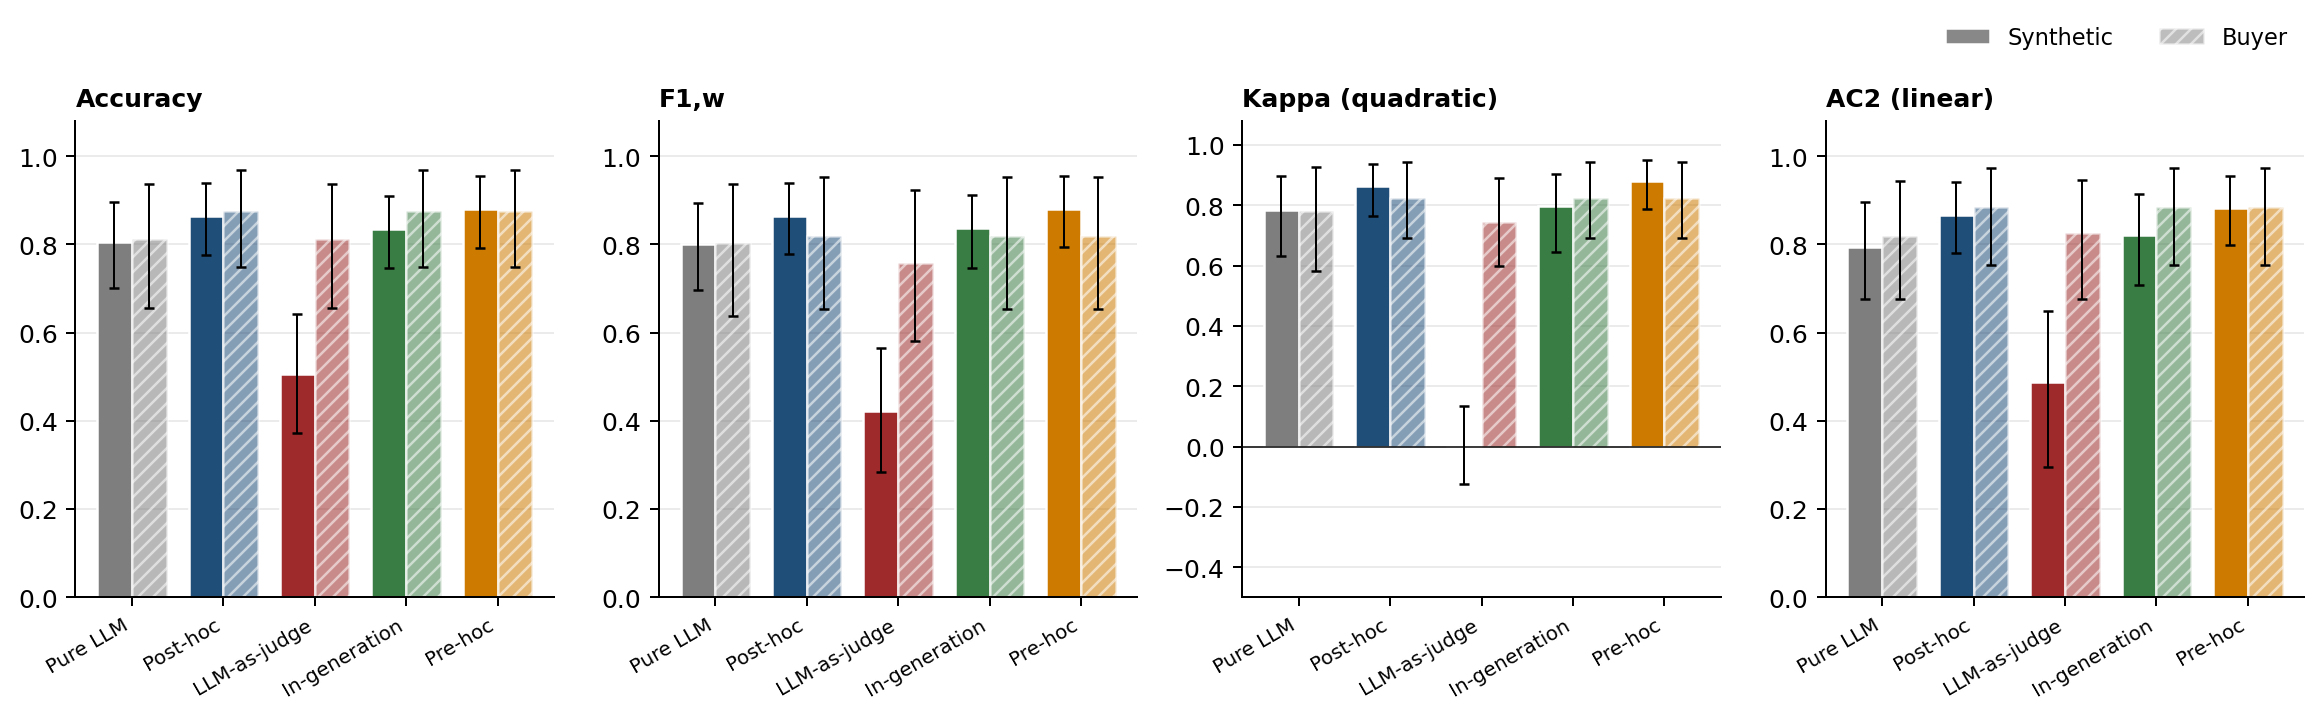
\includegraphics[width=0.85\textwidth]{Figures/fig_5_metrics_grid.png}
\caption{Disposition metrics by design: synthetic (solid) and buyer (hatched), with 95 per cent bootstrap intervals.}
\label{fig:results:metrics}
\end{figure}

\begin{figure}[htb]
\centering
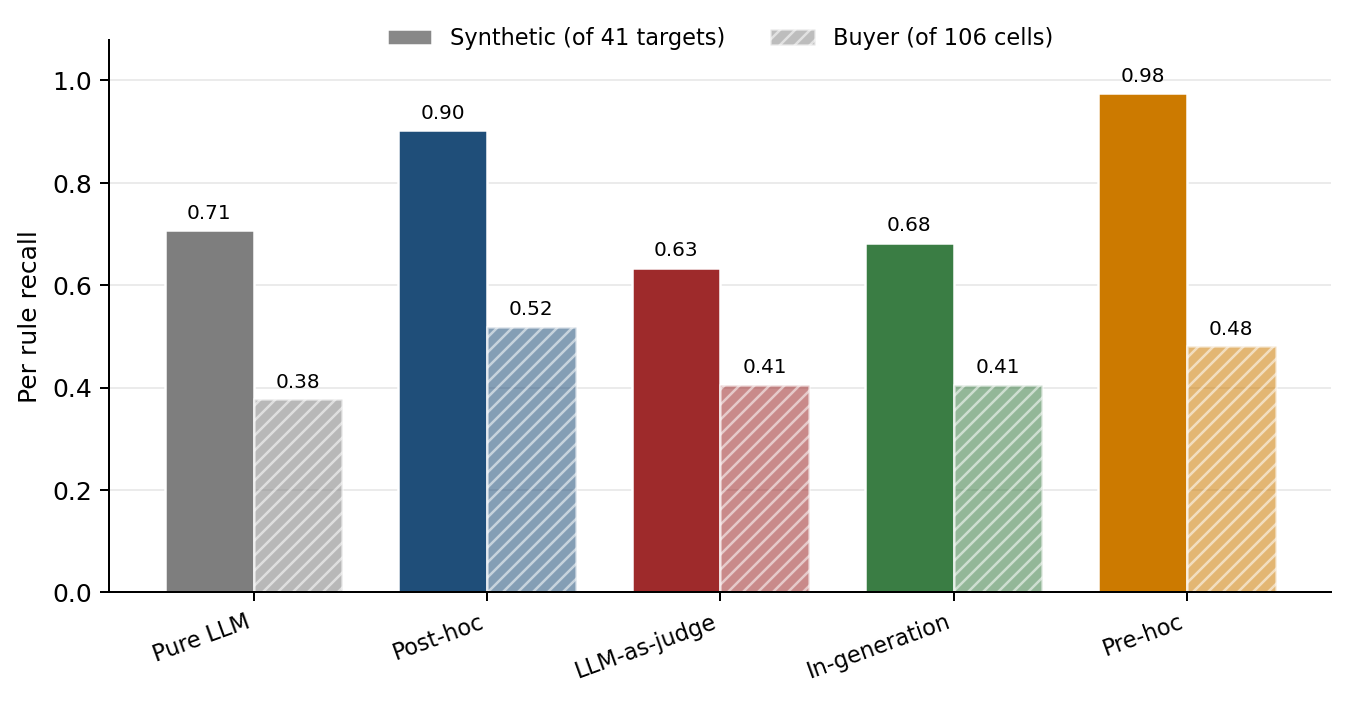
\includegraphics[width=0.8\textwidth]{Figures/fig_5_recall_bars.png}
\caption{Per rule recall by design on the synthetic sample (over the 41 evaluable single rule mutant targets) and the buyer sample (over 106 rule cells). R11 and R18 are excluded (Section~\ref{sec:results:regimes}).}
\label{fig:results:recallbars}
\end{figure}

On the synthetic sample, 3 things stand out. First, 4 of the 5 designs score between 0.81 and 0.88 on accuracy, but the LLM-as-judge design collapses to 0.51, with a weighted kappa of $-0.01$ (chance level). It is consistently too harsh: 28 of its 33 errors are over-rejections, and it fails all 9 clean single rule PASS controls, where every other design passes 6 or 7. Second, the 2 designs that route every deterministic rule through the enforcer lead on rule recall, pre hoc at 40 of 41 and post hoc at 37 of 41, against 26 to 29 for the rest. Third, accuracy and rule recall do not track each other, because a disposition turns only on the most severe firing while recall needs every target firing caught; this is why the in generation design reaches 0.84 accuracy but only 0.68 recall.

On the buyer sample the designs fall into 2 bands. The 3 enforcer bearing designs all reach 0.88 accuracy and are identical on the other 3 metrics; the 2 enforcer free designs reach 0.81. So the metrics separate enforcer from no-enforcer, but they do not separate the 3 enforcer positions. Those 3 differ only on rule recall: post hoc catches 55 of the 106 rule cells, pre hoc 51 and in generation 43. Post hoc leads here because its override recovers missed firings while keeping the model's own answers on the language model rules.


\subsection{Multi-rule interaction scenarios}
\label{sec:results:multirule}

The 17 multi-rule scenarios (SYN-M01 to SYN-M17) place 2 or 3 defects on the same ASN at once, to test whether each design still reaches the correct disposition when violations interact. Table~\ref{tab:synthetic_multirule} reports the outcome. The designs are close: the pure LLM design gets 16 of 17 right and the 3 enforcer bearing designs 15 each. Two scenarios account for the misses. SYN-M13, an intended clean PASS control, is routed to REVIEW by every design because the generated fixture carries inadvertent triggers, an early delivery placed before a fixed notice date and a within tolerance quantity that the line total check still flags, so it tests the fixture rather than the designs. SYN-M10 is missed only by the 3 enforcer designs: its partial shipment is routed to REVIEW where the construction expects REJECT, the same partial-shipment grading tension dissected for case P-48 (Section~\ref{sec:results:p48}). The LLM-as-judge design is again weakest at 13 of 17. Rule coverage, the share of the 38 stacked defects (2 or 3 per scenario across the 17 scenarios) each design flags, matters less, since the disposition turns on the single most severe firing; here the post hoc and pre hoc designs catch 34 of 38, against 27 for the LLM-as-judge design. The gaps are small, 1 to 3 scenarios, but the direction matches the single rule block: the LLM-as-judge design again loses the most dispositions.

\begin{table}[htb]
\centering
\caption{Multi-rule scenarios (SYN-M01--M17): correct dispositions and stacked-firing coverage per design. R18 tracker artefacts are excluded from coverage.}
\label{tab:synthetic_multirule}
\footnotesize
\begin{tabular}{@{}lccl@{}}
\toprule
\textbf{Design} & \textbf{Disposition match} & \textbf{Rule coverage} & \textbf{Scenarios missed} \\
\midrule
pure LLM      & 16/17 & 31/38 & SYN-M13 \\
post hoc      & 15/17 & 34/38 & SYN-M10, SYN-M13 \\
LLM-as-judge  & 13/17 & 27/38 & SYN-M02, SYN-M04, SYN-M12, SYN-M13 \\
in generation & 15/17 & 28/38 & SYN-M10, SYN-M13 \\
pre hoc       & 15/17 & 34/38 & SYN-M10, SYN-M13 \\
\bottomrule
\end{tabular}
\end{table}


\subsection{Paired contrasts between designs}
\label{sec:results:significance}

The paired contrasts take the pre hoc design as the reference. The McNemar test is symmetric, so the p-value and Cohen's h of a pair do not depend on which design is named the reference; the choice only fixes which 4 contrasts form the Holm-corrected family. Pre hoc is the natural anchor because it is the design this study recommends, the one that matches the others on disposition agreement while leading on cost, latency and reproducibility (Section~\ref{sec:results:position}), so each contrast asks the decision relevant question: does any alternative differ from the design that would be deployed? The 4 contrasts map onto the research questions: against the pure LLM baseline and the LLM-as-judge auditor for RQ.1, and against the post hoc and in generation realisations for RQ.2.

The full paired contrast table, with discordant counts, McNemar p-values and Cohen's h for every pair on both samples, is in Appendix~\ref{app:dispmetrics} (Table~\ref{tab:results:significance}).

One contrast survives correction: on the synthetic sample the pre hoc design beats the LLM-as-judge design on 27 discordant cases to 2, with an exact McNemar p below 0.001 after Holm and a large effect size of h equal to 0.85. Every other contrast is negligible to small and none other survives correction; against the post hoc and in generation realisations the discordant counts are tiny (2/1 and 4/1 on synthetic, 0/0 on buyer), so the 3 enforcer positions are indistinguishable. The single reliable separation is therefore the collapse of the LLM auditor, not a ranking among the enforcer positions. Figure~\ref{fig:results:forest} shows this: only the synthetic LLM-as-judge contrast clears the large effect band.

As a check, the same comparisons were run again on all 100 cases together. The judge design still fails clearly, and the 3 enforcer positions are still too close to separate, so combining the buyer and synthetic samples tells the same story. The main accuracy comparisons are not combined this way, because the number of synthetic cases was a design choice, and adding them in would make the result look stronger than the real case evidence supports.

\begin{figure}[htb]
\centering
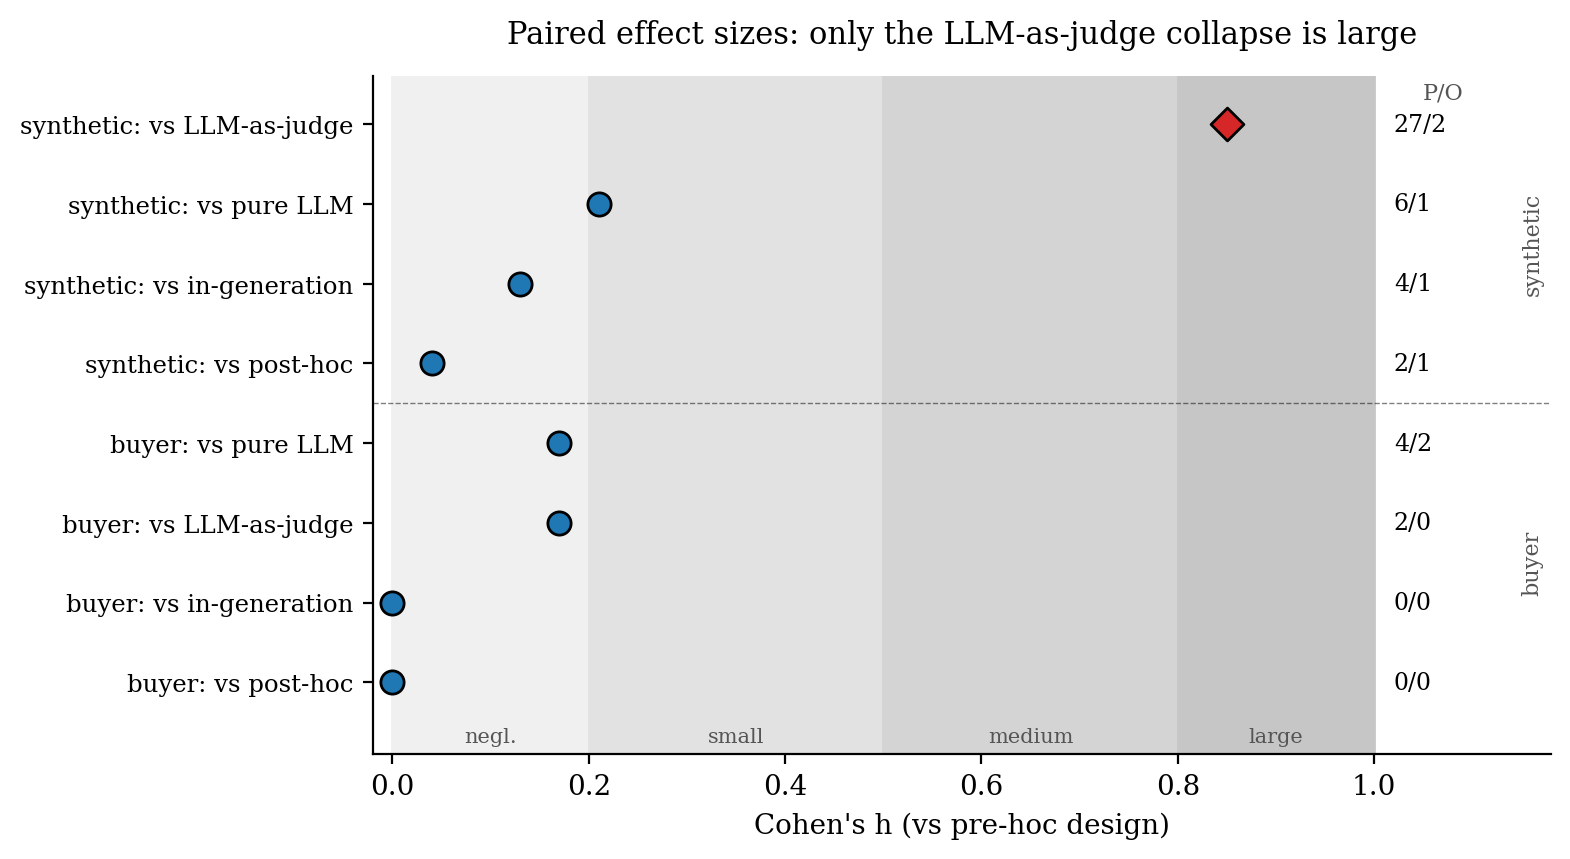
\includegraphics[width=0.86\textwidth]{Figures/fig_5_forest.png}
\caption{Paired effect sizes (Cohen's h) against the pre hoc reference. Only the synthetic LLM-as-judge contrast is large and Holm-significant.}
\label{fig:results:forest}
\end{figure}


\subsection{Per rule behaviour, rule regimes and severity-weighted F1}
\label{sec:results:regimes}

Per rule behaviour spans 2 rule populations: the 8 deterministic regime rules, whose verdict the enforcer can override, and the 14 language model regime rules, whose verdict only the model produces. In the pure LLM and LLM-as-judge designs the deterministic regime rules are left to the model, so their figures show how the model alone does on the rules the others enforce.

This is where the enforcer's advantage lies. Across the 20 evaluable rules, post hoc and pre hoc catch all 20, pure LLM 16, and in generation and LLM-as-judge 14 each. The misses concentrate on a few computation heavy rules that need a recomputed severity, a cumulative quantity or a careful field read: R06 (line item completeness), R17 (multi-PO consolidation), R20 (weight plausibility), R21 (mandatory packaging fields) and R22 (cumulative order fulfilment). Of these only R06 sits in the deterministic regime, where the enforcer recomputes it directly; the others remain in the language model regime, so the enforcer bearing designs recover them through the model rather than by deterministic recomputation, most cleanly under pre hoc, where scoping the model to fewer rules lifts its performance on them. Its value is therefore concentrated on a handful of rules the model handles unreliably under full instruction density, not on the register as a whole.

The 2 rules outside the recall count behave as expected: R11 (schema compliance) is an entry check that yields no rule level verdict, and R18 (duplicate submission) is caught by the separate re-submission check of Section~\ref{sec:method:enforcer:realisations}, where the 3 designs carrying the deterministic tracker flag the engineered duplicate and the pure LLM design does not. The severity weighted macro F1 by rule regime is in Appendix~\ref{app:dispmetrics} (Table~\ref{tab:results:fwslices}); it runs lower than the disposition accuracies because it averages over every rule, including rarely firing ones, and its ordering matches the recall table.


\subsection{Cost and latency}
\label{sec:results:cost}

Cost and latency are observed on the 28 production cases, the recurring operating stream; the 4 pre-integration cases are one-off integration events, excluded here but kept in the 32 case disposition results, and the synthetic cases do not represent live cost. The full operational spread is in Appendix~\ref{app:operational}, together with the latency distribution (Figure~\ref{fig:results:latency}) and the cost/accuracy trade-off (Figure~\ref{fig:results:pareto}).

The pre hoc design is the cheapest and fastest by a clear margin, at EUR 0.073 per ASN and a median latency of 7.89 seconds, and its distribution is the tightest, with a latency standard deviation of 1.73 seconds against 5.70 or more for every other design. The in generation design is the most expensive, at EUR 0.171 per ASN, a cost ratio of 2.34 against the pre hoc design. The reason is prompt size: the pre hoc design fixes the deterministic verdicts before the model call and asks the model to reason over the language model rules only (prompt mean 9,870 tokens), while the in generation design carries tool definitions in the prompt and interleaves tool calls in the response (prompt mean 26,244 tokens).

At this throughput the absolute compute cost is small, and the operationally significant saving is the analyst time the pipeline removes, the same for every design because they share the disposition output. Chapter~\ref{chap:conclusions} works that saving through and weighs it against the compute cost.


\subsection{Supplier context ablation}
\label{sec:results:rag}

This subsection answers RQ.3, whether conditioning the prompt on a supplier's historical failure record improves disposition accuracy. The supplier conditioned prompting layer injects a retrieved supplier history line into the prompt; the method, including the leave-one-out and placebo protocol, is defined in Section~\ref{sec:method:supplier}. Its effect is isolated by an ablation on the 18 production cases swept under all arms: retrieval off, retrieval on under a leave-one-out protocol, and a wrong supplier placebo. Table~\ref{tab:rag_ablation} reports disposition accuracy and the language model regime F1, the only rules the prior can move. The placebo arm is run only for the enforcer free designs (pure LLM and LLM-as-judge): it isolates whether the model is swayed by an authoritative-looking but wrong history, a property of the model that the enforcer would override anyway, so n/a marks the arm as not run rather than missing for the enforcer bearing designs.

\begin{table}[htb]
\centering
\caption{Supplier context ablation on 18 production cases: disposition accuracy and language model-regime F1 across retrieval off, on (leave-one-out) and placebo.}
\label{tab:rag_ablation}
\footnotesize
\begin{adjustbox}{max width=\textwidth}
\begin{tabular}{@{}lcccccc@{}}
\toprule
& \multicolumn{3}{c}{\textbf{Accuracy}} & \multicolumn{3}{c}{\textbf{LM-regime F1}} \\
\cmidrule(lr){2-4} \cmidrule(lr){5-7}
\textbf{Design} & \textbf{Off} & \textbf{On} & \textbf{Placebo} & \textbf{Off} & \textbf{On} & \textbf{Placebo} \\
\midrule
pure LLM      & 0.778 & 0.778 & 0.778 & 0.365 & 0.352 & 0.357 \\
post hoc      & 0.778 & 0.778 & n/a   & 0.454 & 0.337 & n/a   \\
LLM-as-judge  & 0.667 & 0.667 & 0.611 & 0.332 & 0.337 & 0.344 \\
in generation & 0.667 & 0.778 & n/a   & 0.483 & 0.382 & n/a   \\
pre hoc       & 0.778 & 0.778 & n/a   & 0.358 & 0.278 & n/a   \\
\bottomrule
\end{tabular}
\end{adjustbox}
\end{table}

The measured finding is a null effect, so the answer to RQ.3 is negative on this sample. Accuracy does not move between arms on 4 of the 5 designs, and across all 5 at most 2 of the 18 dispositions change. The prior is read rather than ignored, since it shifts the language model regime F1, but no disposition follows, so the verdict is robust to it.

A strict past-only variant conditions each case only on the supplier's earlier cases, leaving the first case of each supplier cold, so 11 of the 18 cases carry a non-empty prior. This variant reproduces the null. Accuracy stays at the no-context baseline on 4 of the 5 designs and moves by a single case on the other 2, a net of zero flips against the off arm. Removing the look-ahead therefore reveals no hidden benefit, and closes the objection that the leave-one-out result masked a real effect by drawing on future cases. On this sample reliability comes from the deterministic enforcer, not the retrieved supplier context, whether that context is read across all of a supplier's cases or only its past. This is taken up in Chapter~\ref{chap:conclusions}.


\subsection{Cross-model robustness}
\label{sec:results:crossmodel}

The results above use a single language model (Section~\ref{sec:method:constraints}). To test whether the separation between the designs is specific to that model, the buyer cohort was also evaluated under a second model from a different family, Mistral-Large-3 on Azure AI Foundry, holding the pipeline, the prompts and the rule logic fixed. Three provider side settings differ on the second model: the seed and schema constrained outputs are unavailable and were disabled, R18 was excluded from the sweep, and the in generation design needed a transport accommodation to invoke its tools; the deterministic checks themselves are identical. Table~\ref{tab:results:crossmodel} reports disposition accuracy per design on the 32 buyer cases for both models, and Figure~\ref{fig:results:crossmodel} plots the same values as a dot plot.

\begin{table}[htb]
\centering
\caption{Cross-model robustness: disposition accuracy on the 32 buyer cases per design, under the primary model (gpt-5.4-mini) and a second model from a different family (Mistral-Large-3).}
\label{tab:results:crossmodel}
\footnotesize
\begin{tabular}{@{}lcc@{}}
\toprule
\textbf{Design} & gpt-5.4-mini & Mistral-Large-3 \\
\midrule
pure LLM      & 0.81 & 0.69 \\
post hoc      & 0.88 & 0.84 \\
LLM-as-judge  & 0.81 & 0.72 \\
in generation & 0.88 & 0.81 \\
pre hoc       & 0.88 & 0.81 \\
\bottomrule
\end{tabular}
\end{table}

\begin{figure}[htb]
\centering
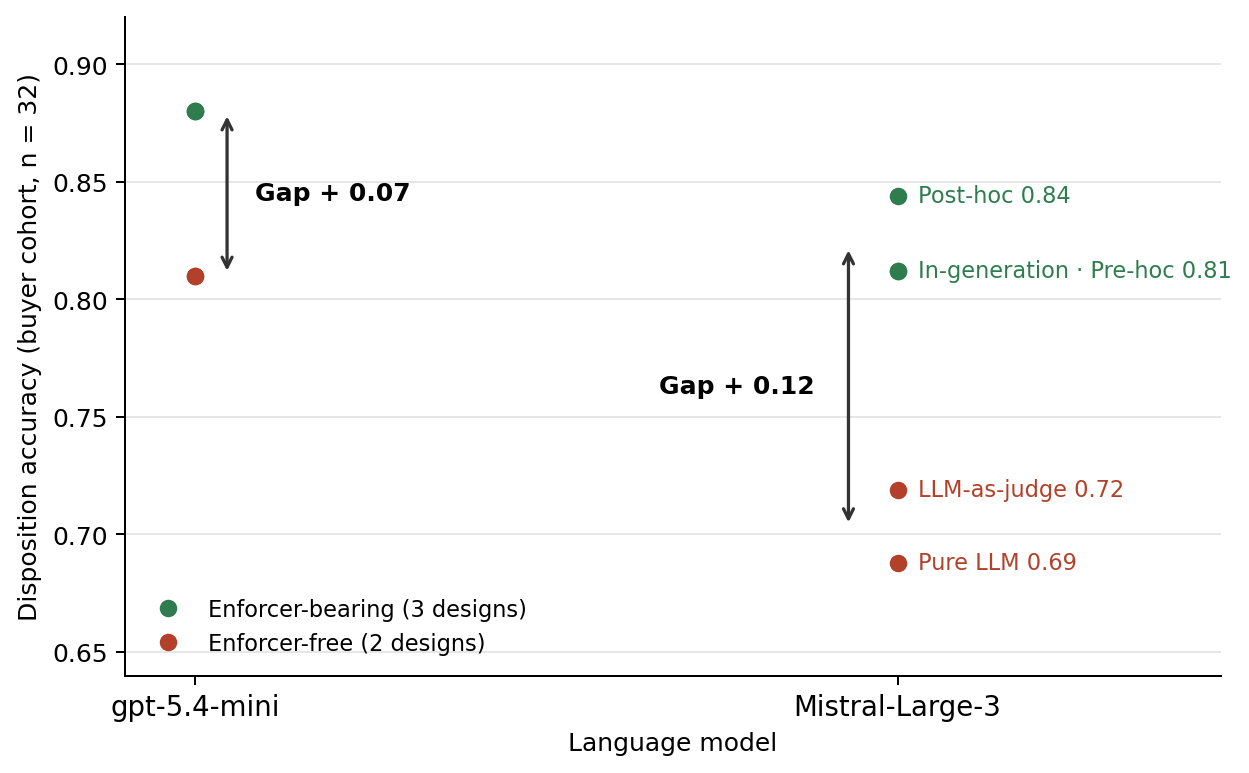
\includegraphics[width=0.82\textwidth]{Figures/fig_5_crossmodel_slopegraph_2.png}
\caption{Cross-model enforcer gap: buyer cohort disposition accuracy of the 5 designs under the primary model (gpt-5.4-mini) and a second model from a different family (Mistral-Large-3).}
\label{fig:results:crossmodel}
\end{figure}

Under Mistral-Large-3 the absolute accuracies are lower, as expected for a model less suited to the task, but the enforcer versus no enforcer separation reproduces and in fact widens. The 3 enforcer bearing designs average 0.82 against 0.70 for the 2 enforcer free designs, a gap of 0.12, against 0.07 on the primary model. The separation is therefore not an artefact of the primary model. The gap widens for a simple reason: the enforcer recomputes the deterministic rules identically regardless of the model, so on a weaker model the enforcer free designs lose more accuracy while the enforcer bearing designs are protected. Practically, this de-risks model choice: a weaker or cheaper model can be deployed behind the enforcer with bounded loss, because the computable rules are protected. The safety asymmetry also replicates only where the enforcer's authority is hard: under the second model the post hoc and pre hoc designs still never under-reject, while the in generation design lets 2 defective ASNs through, so the soft realisation is the first to lose the safety property as the model weakens. The second model also ran several times slower per case on the same pipeline, so the primary model keeps the operational edge. The reported values are the majority of 3 replays per case. Appendix~\ref{app:crossmodel} gives the per-design confusion matrices, the error direction, the reproducibility across replays and the per-run latency on the second model.


%% =================================================================
\section{Position of the deterministic enforcer}
\label{sec:results:position}

The 3 enforcer positions, post hoc, in generation and pre hoc, do not separate on disposition agreement (Section~\ref{sec:results:comparison}): they are identical on the buyer sample and within run-to-run noise on the synthetic one (Table~\ref{tab:results:significance}). The decision between them therefore rests on the operational criteria of RQ.2: cost, latency and reproducibility, and on all 3 the pre hoc design leads. It is the cheapest and the fastest, with the per-design figures in Section~\ref{sec:results:cost}, and the most reproducible, Table~\ref{tab:results:repro} reporting how often each design returns an identical verdict across the 5 runs. Figure~\ref{fig:results:rq2} summarises the answer: the 3 positions overlap on accuracy and separate only on the operational axes, where the pre hoc design leads each one.

\begin{figure}[htb]
\centering
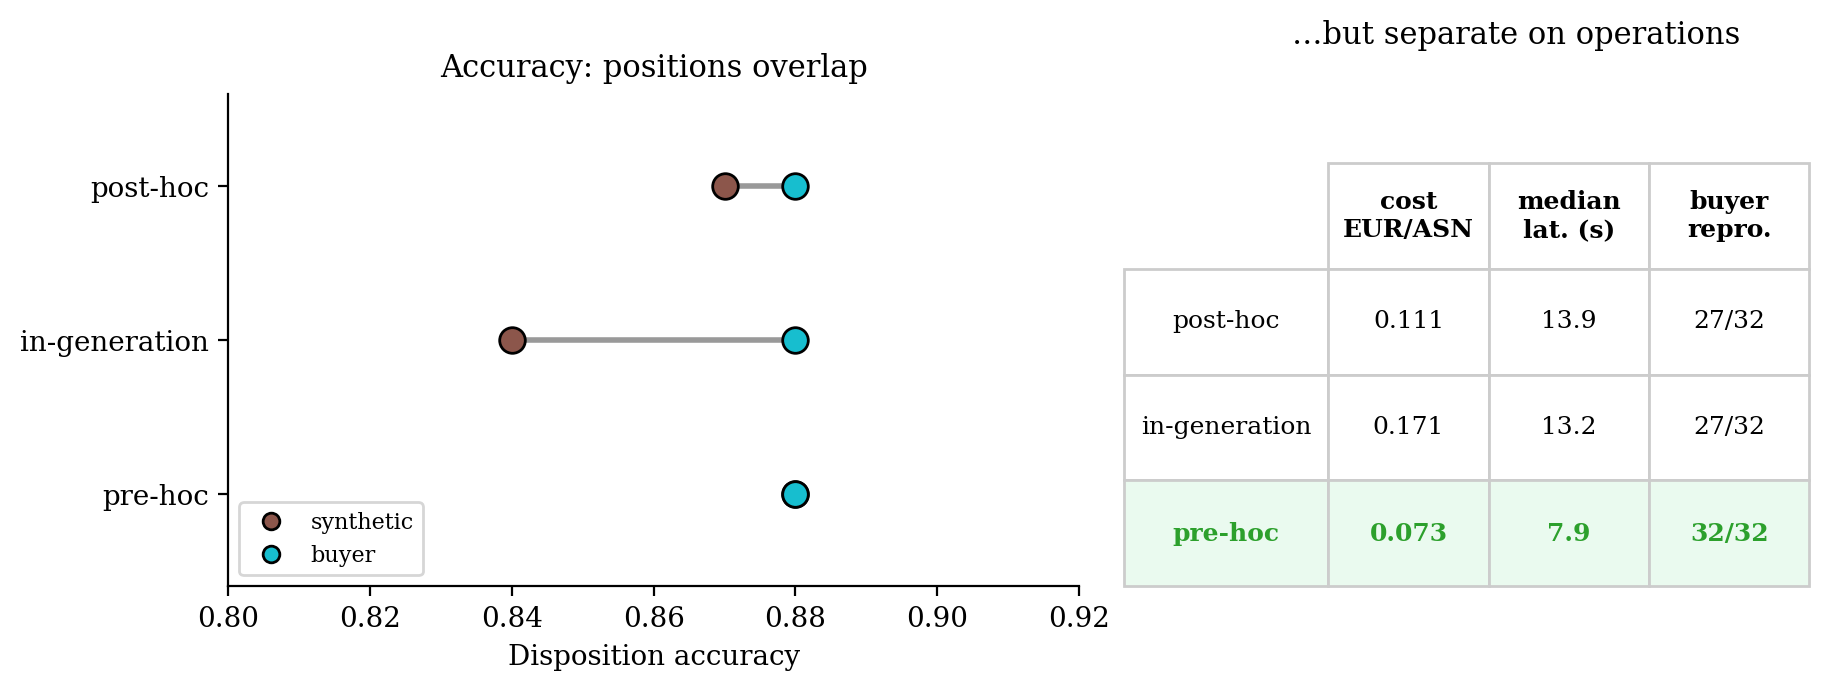
\includegraphics[width=0.85\textwidth]{Figures/fig_5_rq2_dumbbell.png}
\caption{The 3 enforcer positions: identical on accuracy (left), separated only on cost, latency and reproducibility (right), where the pre hoc design leads.}
\label{fig:results:rq2}
\end{figure}

Verdict reproducibility across the 5 runs is reported in Appendix~\ref{app:dispmetrics} (Table~\ref{tab:results:repro}). On the buyer sample the pre hoc design is the only enforcer position whose disposition is identical in all 5 runs, 32 of 32, with a per-run accuracy standard deviation of 0.000. The post hoc and in generation designs each repeat 27 of 32 buyer verdicts, and the post hoc per-run accuracy ranges from 0.81 to 0.94. On the synthetic sample the pre hoc design is again the most stable, at 66 of 67, against 61 of 67 for the post hoc design and 43 of 67 for the LLM-as-judge design, and is therefore the recommended position. The post hoc design retains the per rule recall edge on the buyer sample, 0.52 against 0.48, which matters where the per rule audit trail is the product; this does not change the disposition tie. The in generation design matches the others on agreement but is the most expensive and holds no compensating advantage.

\subsection{What the enforcer does at each position}
\label{sec:results:actions}

The action audit explains why the 3 positions tie on agreement while differing operationally. The post hoc enforcer works downstream, correcting the model after the fact with 32 verdict overrides and 43 missing-firing injections; Table~\ref{tab:results:flow} shows what those corrections achieve against the pure LLM design that shares its model call, lifting the correct count and cutting over-rejections on both cohorts. The in generation design consults the deterministic tools during generation, so overrides are unnecessary and the only residual action is severity capping. The pre hoc design records 0 actions of any kind: by fixing the deterministic verdicts before the model call it prevents the error upstream rather than correcting it downstream, which is also why it leads on cost, latency and reproducibility. The per-design action counts and the severity-capping counterfactual are in Appendix~\ref{app:dispmetrics} (Tables~\ref{tab:results:actions} and~\ref{tab:results:capping}).

\begin{table}[htb]
\centering
\caption{What the post hoc enforcer corrects, against the pure LLM design that shares its model call.}
\label{tab:results:flow}
\footnotesize
\begin{tabular}{@{}lcccccc@{}}
\toprule
& \multicolumn{3}{c}{\textbf{Synthetic (67)}} & \multicolumn{3}{c}{\textbf{Buyer (32)}} \\
\cmidrule(lr){2-4} \cmidrule(lr){5-7}
\textbf{Outcome} & \textbf{pure LLM} & \textbf{post hoc} & \textbf{Change} & \textbf{pure LLM} & \textbf{post hoc} & \textbf{Change} \\
\midrule
Correct dispositions & 54 & 58 & $+4$ & 26 & 28 & $+2$ \\
Over-rejections      & 8  & 5  & $-3$ & 6  & 4  & $-2$ \\
Under-rejections     & 5  & 4  & $-1$ & 0  & 0  & 0    \\
\bottomrule
\end{tabular}
\end{table}

These auxiliary operations are the enforcer's output contract rather than per-design features: whichever realisation runs, injection guarantees no owned rule is missing and capping guarantees its severity matches the register, so they are kept as safety nets against language model non-determinism even where this corpus triggered them 0 times. Where capping changes a disposition it always moves it toward the ground truth. The firing pattern is itself the finding: post hoc corrects after the fact, in generation needs only capping, and pre hoc needs nothing.


%% =================================================================
\section{Error analysis}
\label{sec:results:errors}

\subsection{Error direction}
\label{sec:results:direction}

Disposition errors fall into 2 kinds on the ordered scale PASS, REVIEW, REJECT. An over-rejection is a verdict more severe than the analysts', and an under-rejection is a verdict less severe. The two carry different operational weight: an over-rejection sends a sound ASN to manual review, while an under-rejection lets a defective ASN through. The under-rejection is the unsafe error, because it is the one that reaches the buyer.

On the buyer sample, every error that any design makes is an over-rejection: of the verdicts that differ from the consensus, all are more severe than it and none less severe, as the buyer panel (top row) of Figure~\ref{fig:results:confusion} shows, where every off-diagonal cell sits above the diagonal and none below. The errors split into 2 mechanisms. The first is severity escalation: of the 15 cases the panel marked REVIEW, the pure LLM design pushes 4 to REJECT and the LLM-as-judge design 2, while the 3 enforcer bearing designs push none, because the enforcer recomputes each deterministic rule's registered severity instead of trusting the model's. The second is completeness over-review: of the 4 PASS cases, every design escalates 2 to 4 to REVIEW on packaging completeness grounds (R21, which asks whether the mandatory packaging fields are present), which the enforcer does not suppress, because the question is which rule fires, not how severe. On the synthetic sample, where the mutants engineer genuine defects, under-rejections do occur, 3 to 6 per design, visible below the diagonal in the synthetic panel (bottom row) of Figure~\ref{fig:results:confusion}; the LLM-as-judge design also adds 28 over-rejections, the harshness that Section~\ref{sec:results:p48} dissects.

\begin{figure}[htb]
\centering
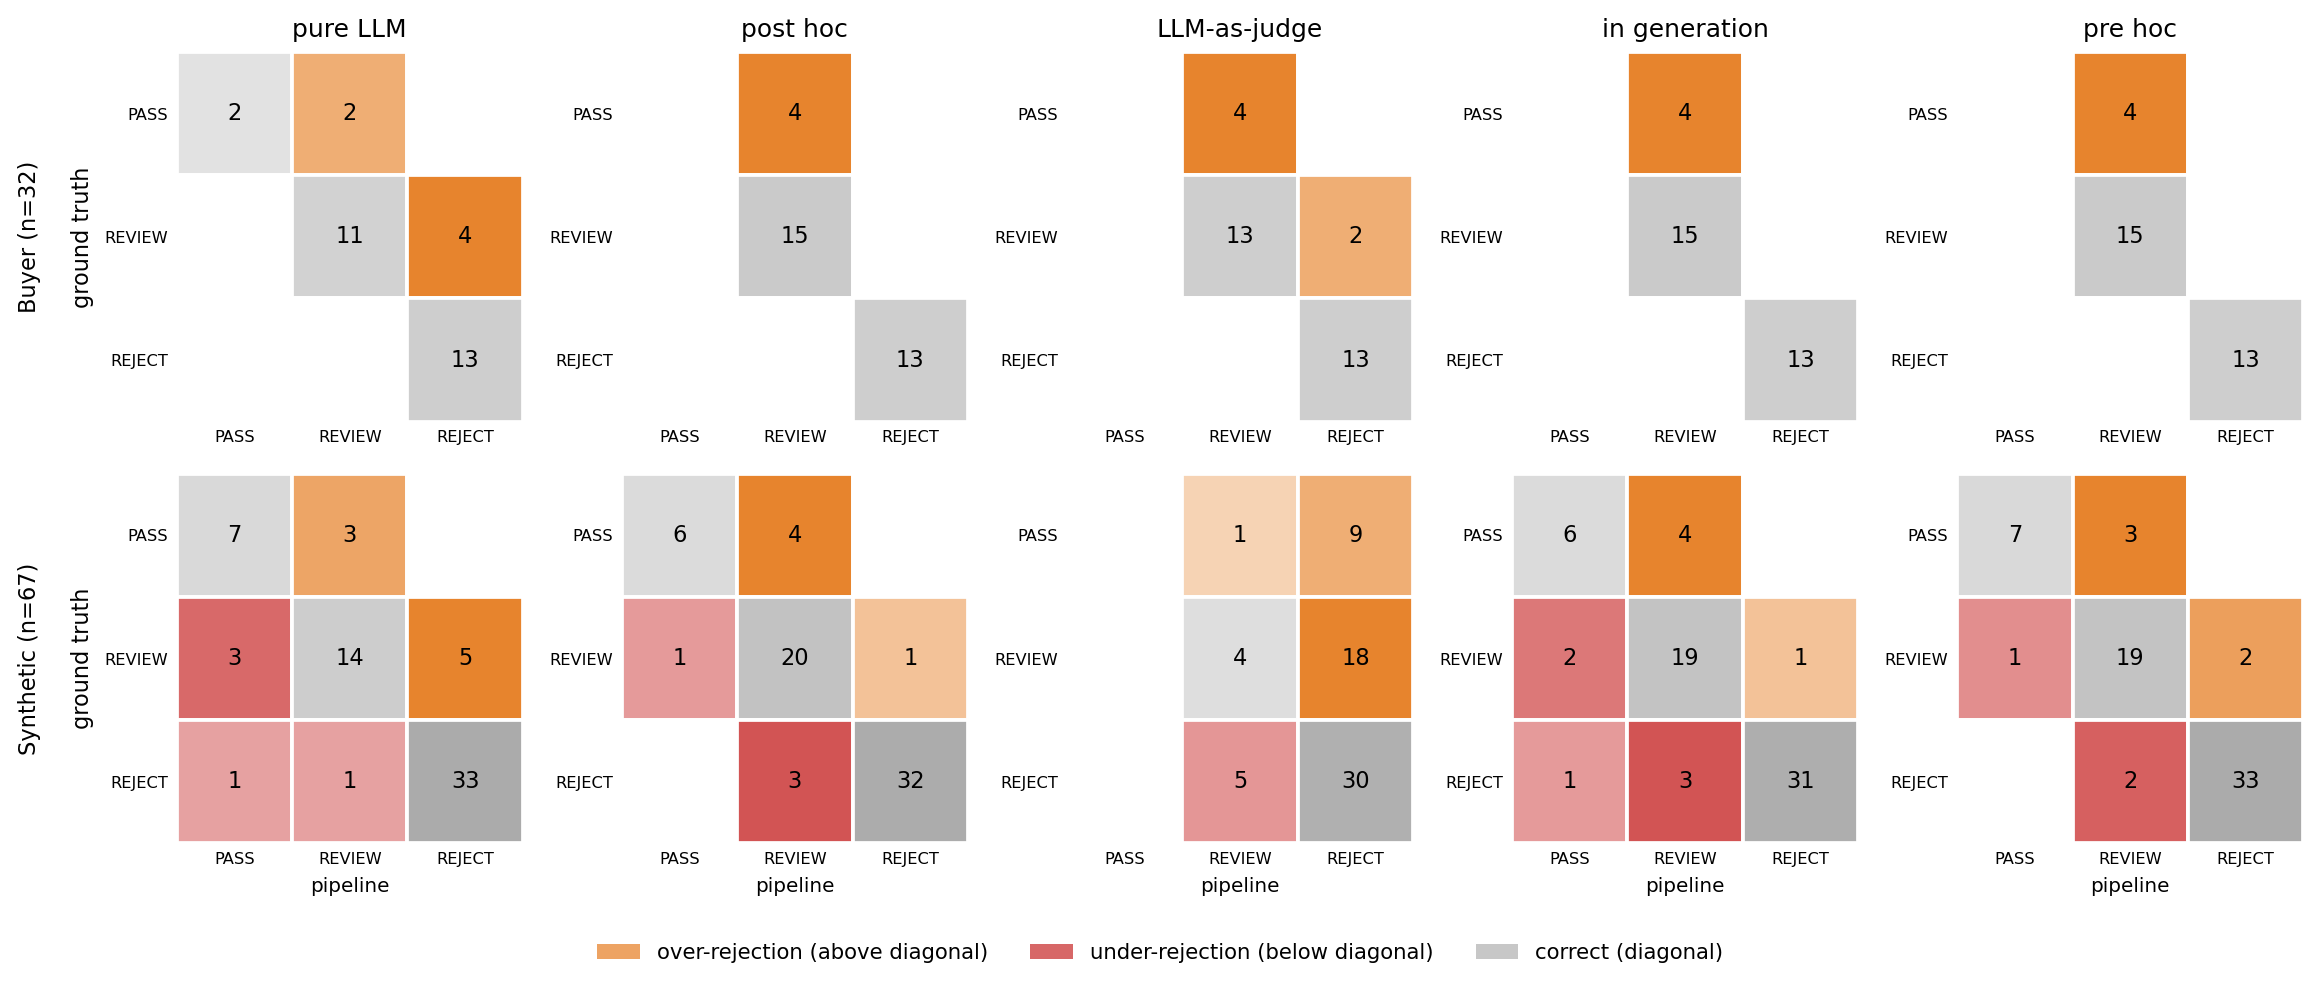
\includegraphics[width=\textwidth]{Figures/fig_5_confusion_panels.png}
\caption{Per-design disposition confusion matrices, buyer cohort (top, n=32) and synthetic cohort (bottom, n=67). Rows are the consensus, columns the pipeline; above the diagonal is over-rejection, below is under-rejection.}
\label{fig:results:confusion}
\end{figure}

Reading the figure, the safety asymmetry is what matters. Over-rejection, the mass above the diagonal, is the tolerable error: a sound ASN is sent to a reviewer, which costs time but never lets a defect through. Under-rejection, below the diagonal, is the unsafe error, because the defect reaches the buyer. No design under-rejects on the buyer cohort, so all 5 are safe in this sense and differ only in how much, and how harshly, they over-review. The 3 enforcer bearing designs keep their only error in the mildest cell, escalating PASS cases to REVIEW on completeness grounds, and never push a genuine REVIEW to REJECT, because the enforcer holds the deterministic severities. The 2 enforcer free designs are harsher: they also bounce genuine REVIEW cases to REJECT, 4 for the pure LLM design and 2 for the LLM-as-judge design, which returns a workable shipment to the supplier and is the costlier over-rejection the enforcer removes.


\subsection{Error walkthrough: cases P-48 and SYN-M10}
\label{sec:results:p48}

Case P-48 is a representative example of the over-rejection pattern, because its rule signature, a multiple purchase order shipment under partial delivery, recurs across the REJECT subset of the buyer sample. It is a shipment from an Austrian supplier covering 4 purchase orders, each only partially delivered. The analysts' verdict is REVIEW, with several warning-level firings and no critical firing.

The designs diverge on the severity of rule R06 (line item completeness, which asks whether every PO line has a matching ASN item), and that severity decides the disposition. R06 fires here because the partial deliveries leave PO lines uncovered, and its deterministic check grades exactly this situation, missing lines that trace to a declared partial delivery, as warning rather than critical. The pure LLM design escalates R06 to critical and returns REJECT. The LLM-as-judge design escalates R06 to critical on all 4 purchase orders, invents a quantity violation (R01, shipped quantity match) by confusing line level and total level quantities, and asserts a duplicate shipment flag (R18) with no supporting evidence, returning REJECT. The 3 enforcer bearing designs all hold R06 at warning, because each routes it through the deterministic enforcer, and all 3 return REVIEW in agreement with the analysts.

Case P-48 exposes 3 independent failure modes of the LLM-as-judge design, each enough on its own to caution against it. It is too harsh: its severity prior runs more severe than the analysts', as the 28 synthetic over-rejections and the 9 of 9 failed single rule PASS controls show. It hallucinates: it invents rule firings with no anchor in the payload, as with R01 and R18 here. And it is unstable: it is the least reproducible design, repeating only 21 of 32 buyer verdicts and 43 of 67 synthetic verdicts. Together with the only Holm-significant contrast in the chapter, these 3 faults rule the pattern out.


The same pattern recurs on the pre-integration sample. The 4 pre-integration cases (PI-01 to PI-04) all carry a consensus REVIEW; 3 are returned REVIEW by every design, while the 4th, PI-04, a partial delivery case, splits the designs exactly as P-48 does: the pure LLM and LLM-as-judge designs escalate it to REJECT, the 3 enforcer bearing designs hold it at REVIEW. The per-case audit is in Appendix~\ref{app:dispmetrics} (Table~\ref{tab:results:pi}).

The same calibration produces the opposite error on the synthetic sample. Scenario SYN-M10 combines a partial shipment with missing packaging fields, and its disposition by construction is REJECT. The 3 enforcer bearing designs return REVIEW, grading the partial shipment as tolerable, while the 2 enforcer free designs reject it. The deterministic severity that grades partial deliveries as warning, and so prevents the over-rejection on P-48, here leaves the case at REVIEW where the construction expects REJECT, and yields an under-rejection. The divergence is confined to this engineered case and does not occur on the buyer cohort, so it marks the boundary of the enforcer's partial-shipment policy rather than a failure on the real sample.



%% =================================================================
\section{Chapter conclusion}
\label{sec:results:conclusion}

This chapter compared the 5 designs on the synthetic and buyer samples. The deterministic enforcer is the component that separates them: the 3 enforcer bearing designs lead on disposition accuracy and rule recall, and the LLM-as-judge design, the only statistically reliable contrast, is ruled out on harshness, hallucination and instability. The 3 enforcer positions tie on disposition agreement, so the choice between them is operational, and the pre hoc design leads on cost, latency and reproducibility. The supplier history prior has no measurable effect, and a second model from a different family reproduces and widens the enforcer gap, confirming the separation is a property of the architecture rather than the model. Chapter~\ref{chap:conclusions} answers the research questions against these findings and sets out the limitations.

% Chapter 6: Conclusion
% Bibliography keys used: gregor2013, sadowski2026, bahroun2026,
% zheng2023, stechly2024, un2030agenda, eurostat2025.

\chapter{Conclusion} \label{chap:conclusions}

This chapter draws the conclusions of the dissertation. Section~\ref{sec:concl:results} summarises the results and answers the 3 research questions. Sections~\ref{sec:concl:practice} and~\ref{sec:concl:research} set out the contributions to practice and to research. Section~\ref{sec:concl:limitations} states the limitations, Section~\ref{sec:concl:future} the avenues for further research, and Section~\ref{sec:concl:sdg} the work's alignment with the Sustainable Development Goals.

\section{Results}
\label{sec:concl:results}

This dissertation designed and evaluated an artefact for the automated validation of advanced shipping notices against their originating purchase orders, a task carried out manually at the partner organisation. Framed as design science research in the improvement quadrant \citep{gregor2013dsr}, the artefact is a staged pipeline that combines a large language model with a deterministic enforcer, evaluated under 5 designs on 67 synthetic and 32 buyer cases.

RQ.1 asks how the 5 designs compare. The deterministic enforcer separates them: the 3 enforcer bearing designs (post hoc, in generation, pre hoc) reach 0.88 buyer accuracy against 0.81 for the 2 enforcer free designs, a gap that widens to 20 points on the synthetic sample, where the LLM-as-judge design collapses, the only statistically reliable contrast. The separation is a property of the architecture, not the model: it reproduces under a second model from a different family (Mistral-Large-3, Section~\ref{sec:results:crossmodel}), where the gap in fact widens rather than closes. Among the 3 enforcer bearing designs accuracy is tied, so the choice between them is settled on operational grounds: the pre hoc design is the one to deploy, matching the top accuracy at the lowest cost and latency, as RQ.2 details.

RQ.2 asks whether the enforcer's position matters. It does not for accuracy, but it does for the operational cost. Position works through the instruction density of the model's prompt, the second knowledge gap Chapter 2 identified: pre hoc settles the 8 deterministic rules upstream and scopes the model to the remaining 14, where post hoc and in generation leave it to reason over all 22. On accuracy no pairwise contrast survives the Holm correction on 32 buyer cases, so the position is immaterial; on operations the gain is large and stable, a cost ratio of 2.34 between pre hoc and in generation. The pre hoc design is therefore the production candidate, matching the top accuracy while leading on cost, latency and reproducibility; the post hoc design is the alternative where per rule coverage and auditability matter more than cost.

RQ.3 asks whether a supplier history prior helps. On this sample it does not: disposition accuracy is unchanged across the off, leave-one-out and placebo arms, and a strict past-only variant reproduces the null. Reliability comes from the deterministic enforcer, not the retrieved context, consistent with the third knowledge gap Chapter 2 identified, that retrieval addresses factuality rather than computational faithfulness. The negative result is itself useful: where the enforcer settles the computable rules, the prior adds little, so engineering effort is better spent on the enforcer than on the prior.

These answers also meet the 3 solution objectives set in Section~\ref{sec:intro:method}. The binary gate is replaced by an auditable, tiered PASS, REVIEW or REJECT disposition (Chapter~\ref{chap:empirical}); every computable rule is settled deterministically in the enforcer bearing designs (Chapter~\ref{chap:method}); and the recommended design runs at EUR 0.073 per ASN and 7.89 seconds median, within a production envelope (Chapter~\ref{chap:results}).

\section{Contribution to Practice}
\label{sec:concl:practice}

For the partner organisation, the artefact replaces a binary accept or reject gate with a staged pipeline and a tiered PASS, REVIEW or REJECT disposition. The current process draws a buyer into a manual reconciliation loop reported at 30 to 90 minutes per defect and 2 to 5 days to resolution; the artefact removes the routine portion of that work and presents an auditable verdict in which the enforcer recomputes every deterministic rule and records why each fired. The recommended configuration is the pre hoc design: cheapest (EUR 0.073 per ASN), fastest (7.89 seconds median), and, like every enforcer bearing design, it is safe on the buyer sample, where its only errors send a sound ASN to review rather than letting a defective one through. For a first deployment this conservative profile is the right one. The cross-model result also means the partner is not locked into one model vendor: the enforcer preserves disposition reliability when the underlying model changes, so the model can be swapped on cost or availability grounds.

The size of that saving can be estimated. A representative month of live production carried 2,331 ASNs, of which 51 failed validation, so of the order of 610 failed ASNs per year each trigger the 30 to 90 minute correction loop. Allowing for the multi-PO handling measured in the sample and an assumed escalation across buyers (Appendix~\ref{app:operational}), automating the detection removes an estimated 570 to 1,700 analyst hours per year, of the order of EUR 22,000 to 65,000 at the partner's loaded hourly cost. The saving is the same for every pipeline design, since all 5 produce the same disposition, and it exceeds the compute cost, of the order of EUR 2,000 per year at the recommended design's per-ASN rate (Section~\ref{sec:results:cost}), by about an order of magnitude. A defect caught on receipt avoids that same correction loop downstream, so the gain is the loop removed rather than a separate downstream cost.

In practical terms, the evidence supports 4 recommendations for the partner organisation:
\begin{itemize}
  \item deploy the pre hoc design, which matches the best accuracy at the lowest cost and latency and is the only design whose verdicts were identical across all repeated runs;
  \item keep the buyer in the loop on every REJECT, since the design's errors are over-rejections and a reviewer recovers them at low cost;
  \item address the supplier REJECT cluster upstream, fixing the recurring currency, transport term and ship-to defects in onboarding and master data;
  \item refresh the supplier profiles from buyer validated audit log entries, so the conditioning layer stays grounded in confirmed dispositions as volume grows.
\end{itemize}

\section{Contribution to Research}
\label{sec:concl:research}

The work makes 3 contributions to research. The first is the formalisation of the enforcer pattern as a reusable architectural component for language model based document validation: the enforcer is defined independently of the document type and the rule set, as the component that deterministically recomputes the rules whose verdict can be settled by computation and holds authority over the disposition for those rules. Any validation task that mixes judgement rules with computation rules can adopt it, and the design question becomes where in the pipeline the enforcer should act. The pattern's value is model agnostic, as the cross-model replication shows. The distinctive element over established in generation tool use, where the model still owns the final verdict, is precisely this deterministic authority, which the enforcer holds when applied post hoc or pre hoc.

The second is the comparison itself. A direct head-to-head comparison of the major hybrid pipeline designs on a single multi-rule structured validation task had been called for explicitly \citep{bahroun2026}, and this dissertation provides it: the 5 designs are evaluated on the same rules, samples and metrics, so the observed differences are attributable to the designs. The placement contrast among the 3 enforcer positions also supplies the first empirical test, in a structured validation setting, of whether reducing instruction density yields accuracy or cost gains, the question Chapter 2 identified as the second knowledge gap.

The third concerns the LLM-as-judge design, whose last place is consistent with the existing judge model literature: judges report high agreement on open-ended comparison \citep{zheng2023} but degrade structured reasoning outcomes \citep{stechly2024}, and document validation is precisely the regime in which a privileged deterministic computation the judge cannot perform makes the judge ineffective. The enforcer's binary verdict, and not its written rationale, is what carries the gain, with the rationale serving the human reviewer in the audit trail.

Beyond these, a smaller contribution is the negative result on supplier conditioning. A controlled ablation, switching a supplier history prior off, on under a leave-one-out protocol, to a placebo and to a strict past-only variant, shows that once a deterministic enforcer settles the computable rules, the prior adds no measurable accuracy. The result bounds where retrieval helps in this regime: it addresses factuality, not the computational faithfulness that document validation turns on.

These contributions close the 3 knowledge gaps Chapter~\ref{chap:lreview} identified, as Table~\ref{tab:concl:gaps} summarises.

\begin{table}[htb]
\centering
\caption{Knowledge gaps of Chapter~\ref{chap:lreview} and how the dissertation closes them.}
\label{tab:concl:gaps}
\footnotesize
\begin{adjustbox}{max width=\textwidth}
\begin{tabular}{@{}p{4.2cm}p{4.6cm}p{4.6cm}@{}}
\toprule
\textbf{Knowledge gap (Chapter 2)} & \textbf{Contribution} & \textbf{Evidence} \\
\midrule
No head-to-head comparison of the major hybrid validation designs & First benchmark of the 5 designs on a single 22-rule task, plus the enforcer pattern & Enforcer bearing designs at 0.88 against 0.81; gap reproduces and widens under a second model (Sections~\ref{sec:results:comparison} and~\ref{sec:results:crossmodel}) \\
Instruction density effects untested in structured validation & First empirical test of enforcer position, which acts through prompt density & Operational gain large and stable, accuracy gain directional (Section~\ref{sec:results:position}) \\
Supplier history grounding untested against a deterministic enforcer & Controlled off/on/placebo ablation with a past-only variant & Null effect on all arms (Section~\ref{sec:results:rag}) \\
\bottomrule
\end{tabular}
\end{adjustbox}
\end{table}

\section{Limitations}
\label{sec:concl:limitations}

The conclusions are qualified by 5 limitations.

\textbf{Sample size.} The samples are small, 67 synthetic and 32 buyer cases, so the bootstrap intervals are wide. On the buyer sample no pairwise accuracy contrast survives the Holm correction; the one statistically reliable contrast in the study, the collapse of the LLM-as-judge design, is on the synthetic sample. A power check confirms the buyer null is a sample size limit rather than evidence of no effect: at n equal to 32 only effects of Cohen's h around 0.70 or larger are detectable, against an observed enforcer gap of about 0.17. The buyer-sample contrasts are therefore read as directional. Combining the two samples would raise the apparent power, but most of the combined set is synthetic and its size was a design choice, so the buyer comparisons are kept on their own.

\textbf{Independence of cases.} The 32 buyer cases are drawn from 19 suppliers and cluster by supplier, so they are not fully independent and the effective sample is smaller than 32. This is a further reason to read the buyer contrasts as directional rather than as significance tests.

\textbf{Ground truth.} The buyer ground truth is a consensus of 3 analysts from the same organisation. Because the analysts share that organisation's conventions, their judgements are not independent of one another, and the reference reflects one organisation's reading of the rules rather than a universal standard. The per analyst labels were reconciled live and only the consensus was retained, so an inter-rater coefficient cannot be computed retrospectively. A panel drawn from several organisations, with the individual labels recorded, would test how far the consensus generalises.

\textbf{Severity specification.} A firing's severity is protected only where the enforcer acts. On the 2 enforcer free designs the model owns severity, and R06 (line item completeness, which asks whether every PO line has a matching ASN item) is the clearest example: its deterministic check grades missing lines as warning when they trace to a declared partial delivery, but the pure LLM and LLM-as-judge designs escalate the same firing to critical and over-reject. This is the mechanism behind most of the over-rejections in Chapter~\ref{chap:results}. Decoupling severity assignment from rule firing, so that severity is owned deterministically even where the verdict needs judgement, would close the gap and is left to future work.

\textbf{Scope.} The study is bounded to one organisation, one document pair (the ASN against its PO) and an offline evaluation. The pipeline was not run in live production, so the buyers' acceptance of its verdicts and their override behaviour are not measured. The cross-model check uses 3 replays per case, fewer than the primary model's 5, and is read as a robustness check rather than a full re-evaluation. How the findings transfer to other document types and to a live deployment is open; order confirmations and invoices are the natural first candidates (Section~\ref{sec:concl:future}).

\section{Avenues for Further Research}
\label{sec:concl:future}

Six directions follow. A larger evaluation would narrow the bootstrap intervals and could settle whether the pre hoc and post hoc designs are genuinely indistinguishable. Extending the analyst panel beyond one organisation would test how far the consensus generalises. Refining the specification so severity is owned deterministically on every design, not only where the enforcer acts, would close the severity gap of Section~\ref{sec:concl:limitations}. A live deployment would measure what the offline evaluation cannot: how readily the buyers accept the pipeline's verdicts and how often they override them. A further direction is to apply the methodology to other procurement documents validated inside the partner organisation, in particular order confirmations and invoices, which share the structure the artefact already handles: a supplier document checked against an order baseline. Because the enforcer pattern is defined independently of the document type (Section~\ref{sec:concl:research}), the architecture should transfer once a rule register is derived for each document, and the arithmetic-heavy invoice check, matched against the purchase order and the goods receipt, is well suited to the deterministic enforcer. Finally, the supplier conditioning layer showed a null effect on the 18 case ablation (Section~\ref{sec:results:rag}); a larger supplier sample and a richer history than the single injected line would establish whether the layer can contribute at all, and given the supplier clustering finding it remains a plausible place to look for further accuracy gains.

\section{Alignment with the Sustainable Development Goals}
\label{sec:concl:sdg}

The work intersects with the United Nations 2030 Agenda for Sustainable Development and its 17 Sustainable Development Goals \citep{un2030agenda}, against which Eurostat monitors EU progress through an annual indicator set \citep{eurostat2025}. Two goals map directly onto the contribution and a third applies indirectly; Table~\ref{tab:concl:sdg} summarises the alignment, the specific targets, and the indicators through which the impact can be measured. The SDG 9 contribution is the technological upgrade itself: the artefact upgrades the validation workflow at the document gate, and the enforcer pattern is a reusable component for other validation tasks, measured by the cost and latency per validated ASN (Section~\ref{sec:results:cost}). The SDG 8 contribution is the one the study quantifies: the labour saving of Section~\ref{sec:concl:practice}, of the order of 570 to 1,700 analyst hours per year on the live volume, is the work's primary measured impact.

The SDG 12 alignment is contextual: the work does not measure environmental impact directly, and the indicator reflects reporting capability rather than measured environmental outcome.

\begin{table}[!ht]
\centering
\caption{Alignment with the Sustainable Development Goals: targets, contribution and indicators.}
\label{tab:concl:sdg}
\small
\setlength{\tabcolsep}{5pt}
\renewcommand{\arraystretch}{1.25}
\begin{tabularx}{\textwidth}{@{}>{\raggedright\arraybackslash}p{2.8cm}>{\raggedright\arraybackslash}p{2.9cm}>{\raggedright\arraybackslash}X>{\raggedright\arraybackslash}X@{}}
\toprule
\textbf{SDG} & \textbf{Target} & \textbf{Contribution} & \textbf{Indicator and metric} \\
\midrule
9. Industry, Innovation and Infrastructure & 9.5, upgrading technological capabilities & Upgrades the validation workflow at the document gate; the enforcer pattern is a reusable component for other validation tasks & Cost and latency per validated ASN (EUR 0.073 per ASN, 7.89\,s median), measured in Chapter~\ref{chap:results} \\
\addlinespace
8. Decent Work and Economic Growth & 8.2, productivity through technological upgrading & Removes the routine portion of defect handling; analysts shift from repetitive reconciliation to the cases that need judgement & Analyst hours saved per year, of the order of 570 to 1{,}700 for the live volume (Section~\ref{sec:concl:practice}) \\
\addlinespace
12. Responsible Consumption and Production & 12.6, corporate sustainability practices and reporting & The structured audit log supports reporting; supplier clustering directs upstream master data fixes & Share of dispositions with a full audit trail, every disposition by construction \\
\bottomrule
\end{tabularx}
\end{table}

%------------Bibliography------------%
\begin{singlespace}
  \renewcommand{\bibname}{References}
  \bibliographystyle{apalike}
  \cleardoublepage%
  \phantomsection%
  \addcontentsline{toc}{chapter}{References}
  \bibliography{7_bibliography}
\end{singlespace}

%---------Appendices-----------------%
\begin{singlespace}
\appendix
%% =====================================================================
%%  A_Appendix1.tex  --- Appendix A: Rule Register and Prompt Examples
%% =====================================================================

\chapter{Methodology supporting material} \label{app:rules}

This appendix gathers the supporting material for the methodology of Chapter~\ref{chap:method}: the complete rule register and failure-mode taxonomy (A.1), prompt technique examples (A.2), the deterministic tools and enforcer action types (A.3), reproducibility and availability (A.4), the metric definitions (A.5), and the evaluation benchmarks reviewed in Chapter~\ref{chap:lreview} (A.6).

\section*{A.1\quad Complete rule register (R01--R22)}

Table~\ref{tab:app:rules} lists every validation rule used in the pipeline, together with its category, severity, one-line check description, and regime assignment.

\footnotesize
\begin{longtable}{@{}cp{3.2cm}p{1.8cm}p{1.8cm}p{4.2cm}p{2cm}@{}}
\caption{Complete rule register (R01--R22).} \label{tab:app:rules} \\
\toprule
\textbf{Rule} & \textbf{Name} & \textbf{Category} & \textbf{Severity} & \textbf{Check (one line)} & \textbf{Regime} \\
\midrule
\endfirsthead
\caption[]{Complete rule register (R01--R22) --- \emph{continued}.} \\
\toprule
\textbf{Rule} & \textbf{Name} & \textbf{Category} & \textbf{Severity} & \textbf{Check (one line)} & \textbf{Regime} \\
\midrule
\endhead
\midrule
\multicolumn{6}{r}{\emph{Continued on next page}} \\
\endfoot
\bottomrule
\endlastfoot
R01 & Shipped quantity match        & Arithmetic  & Critical      & ASN shipped quantity within the PO tolerance band                                        & Deterministic \\
R02 & Unit price match              & Arithmetic  & Critical      & ASN unit price within the PO tolerance band                                              & Deterministic \\
R03 & Delivery date feasibility     & Arithmetic  & Warning       & ASN delivery date within the PO tolerance window                                         & Deterministic \\
R04 & Shipment date realism         & Arithmetic  & Warning       & shipmentDate not in the past relative to noticeDate; deliveryDate $\geq$ shipmentDate; requires date coherence judgement    & Language model \\
R05 & UOM consistency               & Structural  & Critical      & ASN unit of measure matches the PO exactly                                               & Language model \\
R06 & Line item completeness        & Structural  & Crit.\ (downgr.) & Every PO line in the portion has a corresponding ASN item; graded warning when the missing lines trace to a declared partial delivery & Deterministic \\
R07 & No phantom lines              & Structural  & Critical      & ASN contains no item referencing a non-existent PO line                                  & Language model \\
R08 & Currency match                & Structural  & Critical      & ASN currency matches the PO at header and line level                                     & Language model \\
R09 & Supplier ID validation        & Structural  & Critical      & ASN supplier network ID matches the PO supplier network ID                               & Language model \\
R10 & PO reference integrity        & Structural  & Critical      & Each portion references a valid, existing PO orderID                                     & Language model \\
R11 & Schema compliance             & Structural  & Informational & ASN is valid cXML and parsed without errors                                              & Language model \\
R12 & Mandatory field presence      & Structural  & Warning       & Required ASN header and item fields are present                                          & Language model \\
R13 & Transport terms match         & Semantic    & Warning       & ASN incoterms match the PO incoterms                                                     & Language model \\
R14 & Ship-to address match         & Semantic    & Warning       & ASN ship-to address matches the PO ship-to address                                       & Language model \\
R15 & Total value reconciliation    & Arithmetic  & Warning       & qty $\times$ unitPrice matches the PO line total within tolerance                        & Deterministic \\
R16 & Partial-shipment handling     & Arithmetic  & Info.\ (esc.) & Partial shipment flagged with remaining quantity; escalates when R01 detects under-ship   & Deterministic \\
R17 & Multi-PO consolidation        & Structural  & Warning       & Cross-PO boundary integrity for multi-PO ASNs                                            & Language model \\
R18 & Duplicate ASN detection       & Structural  & Critical      & shipmentID + PO set not previously seen (persisted state)                                & Deterministic \\
R19 & ShipmentID length             & Structural  & Critical      & shipmentID $\leq$ 35 characters                                                         & Deterministic \\
R20 & Weight plausibility           & Arithmetic  & Warning       & grossWeight $>$ netWeight and grossWeight $\leq$ netWeight $\times$ 10                   & Language model \\
R21 & Mandatory packaging fields    & Structural  & Critical      & Required packaging fields are present                                                    & Language model \\
R22 & Order fulfilment status       & Arithmetic  & Warning       & Total notified quantity does not exceed PO quantity                                       & Language model \\
\end{longtable}
\normalsize

Table~\ref{tab:method:taxonomy} arranges the same register by the taxonomy of failure modes of Section~\ref{sec:method:taxonomy}, placing each rule in its category and severity cell.

\begin{table}[htbp]
\centering
\caption{Taxonomy of failure modes.}
\label{tab:method:taxonomy}
\footnotesize
\begin{adjustbox}{max width=\textwidth}
\begin{tabular}{@{}lp{2.2cm}p{4.2cm}p{5.8cm}@{}}
\toprule
                    & \textbf{Informational} & \textbf{Warning}              & \textbf{Critical} \\
\midrule
\textbf{Arithmetic} & R16                   & R03, R04, R15, R20, R22       & R01, R02           \\
\textbf{Structural} & R11                   & R12, R17                      & R05, R06, R07, R08, R09, R10, R18, R19, R21 \\
\textbf{Semantic}   & ---                   & R13, R14                      & ---                \\
\bottomrule
\end{tabular}
\end{adjustbox}
\end{table}


%% -----------------------------------------------------------------
\section*{A.2\quad Prompt technique examples} \label{app:prompt}

Table~\ref{tab:app:prompt} reproduces illustrative excerpts from the Stage~5 system prompt, one for each of the four prompt engineering techniques described in Section~\ref{sec:method:prompt}.

\begin{table}[htbp]
\centering
\caption{Prompt engineering technique excerpts from the Stage~5 system prompt.}
\label{tab:app:prompt}
\footnotesize
\begin{adjustbox}{max width=\textwidth}
\begin{tabular}{@{}p{3.2cm}p{9.5cm}@{}}
\toprule
\textbf{Technique} & \textbf{Illustrative excerpt} \\
\midrule
Persona prompting      & ``You are an expert procurement validation agent for the partner organisation.'' \\[6pt]
Task decomposition     & Three numbered sub-tasks: (1)~line alignment between ASN and PO, (2)~rule-by-rule evaluation, (3)~semantic analysis of findings that fall outside the rule set. \\[6pt]
Few-shot prompting     & Three worked examples shown before the case to evaluate: a clean ASN (all rules pass), an R01 over-shipment fail, and an R19 shipmentID-too-long fail. \\[6pt]
Chain-of-thought       & ``When checking R01, R02, and R15, show your calculations explicitly.'' \\
\bottomrule
\end{tabular}
\end{adjustbox}
\end{table}


%% -----------------------------------------------------------------
\section*{A.3\quad Deterministic tools (in generation realisation)}

Table~\ref{tab:method:tools} lists the 7 callable tools exposed to the language model in the in generation realisation of Section~\ref{sec:method:enforcer:realisations}, each covering one deterministic regime rule.

\begin{table}[htbp]
\centering
\caption{Deterministic tools available in the in generation realisation.}
\label{tab:method:tools}
\begin{tabular}{@{}ll@{}}
\toprule
\textbf{Tool} & \textbf{Rule(s) covered} \\
\midrule
\texttt{verify\_quantity\_match}     & R01 --- shipped quantity match       \\
\texttt{verify\_price\_match}        & R02 --- unit price match             \\
\texttt{verify\_date\_arithmetic}    & R03 --- delivery date feasibility    \\
\texttt{verify\_line\_completeness}  & R06 --- line item completeness       \\
\texttt{verify\_line\_total}         & R15 --- total value reconciliation   \\
\texttt{verify\_partial\_shipment}   & R16 --- partial shipment handling    \\
\texttt{verify\_shipment\_id\_length}& R19 --- shipmentID length            \\
\bottomrule
\end{tabular}
\end{table}

Table~\ref{tab:method:actions} lists the 3 logged action types the enforcer records on the rule triples, as described in Section~\ref{sec:method:enforcer:aux}.

\begin{table}[htbp]
\centering
\caption{Enforcer action types.}
\label{tab:method:actions}
\footnotesize
\begin{adjustbox}{max width=\textwidth}
\begin{tabular}{@{}lp{11cm}@{}}
\toprule
\textbf{Action} & \textbf{Triggering condition} \\
\midrule
Override          & The deterministic check on a rule in the deterministic regime disagrees with the language model's verdict; the enforcer's verdict prevails. \\
Rule injection    & The language model omits a verdict for a rule. The enforcer inserts the deterministic verdict for rules in the deterministic regime, or a default with a diagnostic note for rules in the language model regime. \\
Severity capping  & The language model returns a severity that differs from the rule's registered severity in Appendix~\ref{app:rules}. The enforcer clamps the severity to the registered value. \\
\bottomrule
\end{tabular}
\end{adjustbox}
\end{table}


%% -----------------------------------------------------------------
\section*{A.4\quad Reproducibility and availability}
\label{app:repro}

The pipeline source code, the rule register, the synthetic generator, and the anonymised evaluation data and run artefacts are released to support replication, at \url{https://github.com/joaosoaresgoncalves/tese_atualizada}. Together with the fixed model, temperature, and seed described in Section~\ref{sec:method:constraints}, this lets every figure and table in Chapter~\ref{chap:results} be regenerated from the released artefacts.


%% -----------------------------------------------------------------
\section*{A.5\quad Disposition and per rule metric definitions}
\label{app:metrics}

This section gives the definitions of the disposition and per rule metrics used in Section~\ref{sec:method:eval}.

The document level agreement metric is Cohen's quadratically weighted kappa,
%
\begin{equation}\label{eq:kappa}
  \kappa_w = 1 - \frac{\sum_{ij} w_{ij}\, p_{o,ij}}{\sum_{ij} w_{ij}\, p_{e,ij}}
\end{equation}
%
where $p_{o,ij}$ is the observed proportion of documents falling in cell $(i,j)$ of the disposition confusion matrix, $p_{e,ij}$ is the proportion expected if the pipeline and the expert decided independently, and $w_{ij} = (i-j)^2/(k-1)^2$ is the quadratic weight, with $k=3$ the number of categories. The coefficient equals~1 when the pipeline and the expert agree on every document, and~0 when their agreement is no better than chance.

The per rule summary metric is the severity weighted macro F1,
%
\begin{equation}\label{eq:f1w}
  F_{1,w} = \frac{\sum_i w_i\, F_{1,i}}{\sum_i w_i}
\end{equation}
%
with $F_{1,i}$ the F1-score of rule~$i$ and $w_i$ its severity weight (1~for informational, 2~for warning, 3~for critical), so that rules whose failure carries higher operational consequence weigh more in the aggregate.


%% -----------------------------------------------------------------
\section*{A.6\quad Evaluation benchmarks from the literature}

Table~\ref{tab:lr:benchmarks} catalogues the evaluation benchmarks and frameworks reviewed in Section~\ref{sec:lr:sota:benchmarks}.

\begin{table}[htbp]
\centering
\caption{Evaluation benchmarks and frameworks relevant to hybrid validation pipelines.}
\label{tab:lr:benchmarks}
\footnotesize
\begin{adjustbox}{max width=\textwidth}
\begin{tabular}{@{}p{2.1cm}p{2.6cm}p{6.3cm}p{2.6cm}@{}}
\toprule
\textbf{Benchmark} & \textbf{Focus} & \textbf{Key feature} & \textbf{Reference} \\
\midrule
RAGAS           & RAG evaluation                                  & Reference-free modular metrics (faithfulness, context relevance, answer relevance)                              & \citet{es2024}                       \\
ARES            & RAG evaluation                                  & Fine-tuned LLM judges with prediction-powered inference; $\sim$150 (150--300 recommended) human-annotated datapoints & \citet{saadfalcon2024}            \\
TabFact         & Table fact verification                         & 118,275 statements against 16,573 tables; linguistic + symbolic reasoning                                       & \citet{chen2020tabfact}              \\
FEVEROUS        & Fact verification over unstructured + tabular evidence & Hybrid-evidence fact verification                                                                       & \citet{aly2021}                      \\
TAT-QA / FinQA  & Numerical reasoning over tables + text          & Financial QA benchmarks                                                                                        & \citet{zhu2021}; \citet{chen2021finqa} \\
FinanceBench    & Financial QA                                    & 10,231 expert-annotated triplets from SEC filings; GPT-4 errors on 81\%                                         & \citet{islam2023}                    \\
OHRBench        & OCR-to-RAG cascading errors                     & 8,561 document images; quantifies OCR error propagation through RAG                                             & \citet{zhang2025ocr}                 \\
FActScore       & Factual precision                               & Atomic fact decomposition; fine-grained per-claim verification                                                 & \citet{min2023factscore}             \\
JSONSchemaBench & Constrained decoding                            & Six frameworks on real world JSON schemas                                                                      & \citet{geng2025}                     \\
IFScale         & Instruction density                             & Scales 10--500 instructions; measures LLM degradation at high density                                          & \citet{jaroslawicz2025}              \\
\bottomrule
\end{tabular}
\end{adjustbox}
\end{table}

%% =====================================================================
%%  A_Appendix2.tex --- Appendices for Chapter 4 (Empirical Study)
%% =====================================================================

%% -----------------------------------------------------------------
%%  Appendix B --- AS-IS swimlane with pain points
%% -----------------------------------------------------------------
\chapter{AS-IS process with annotated pain points} \label{app:emp:asis}

This appendix reproduces the AS-IS PO--ASN validation swimlane of Section~\ref{sec:emp:asis}, annotated with the 8 pain point markers from Table~\ref{tab:emp:painpoints}.

\begin{figure}[htbp]
\centering
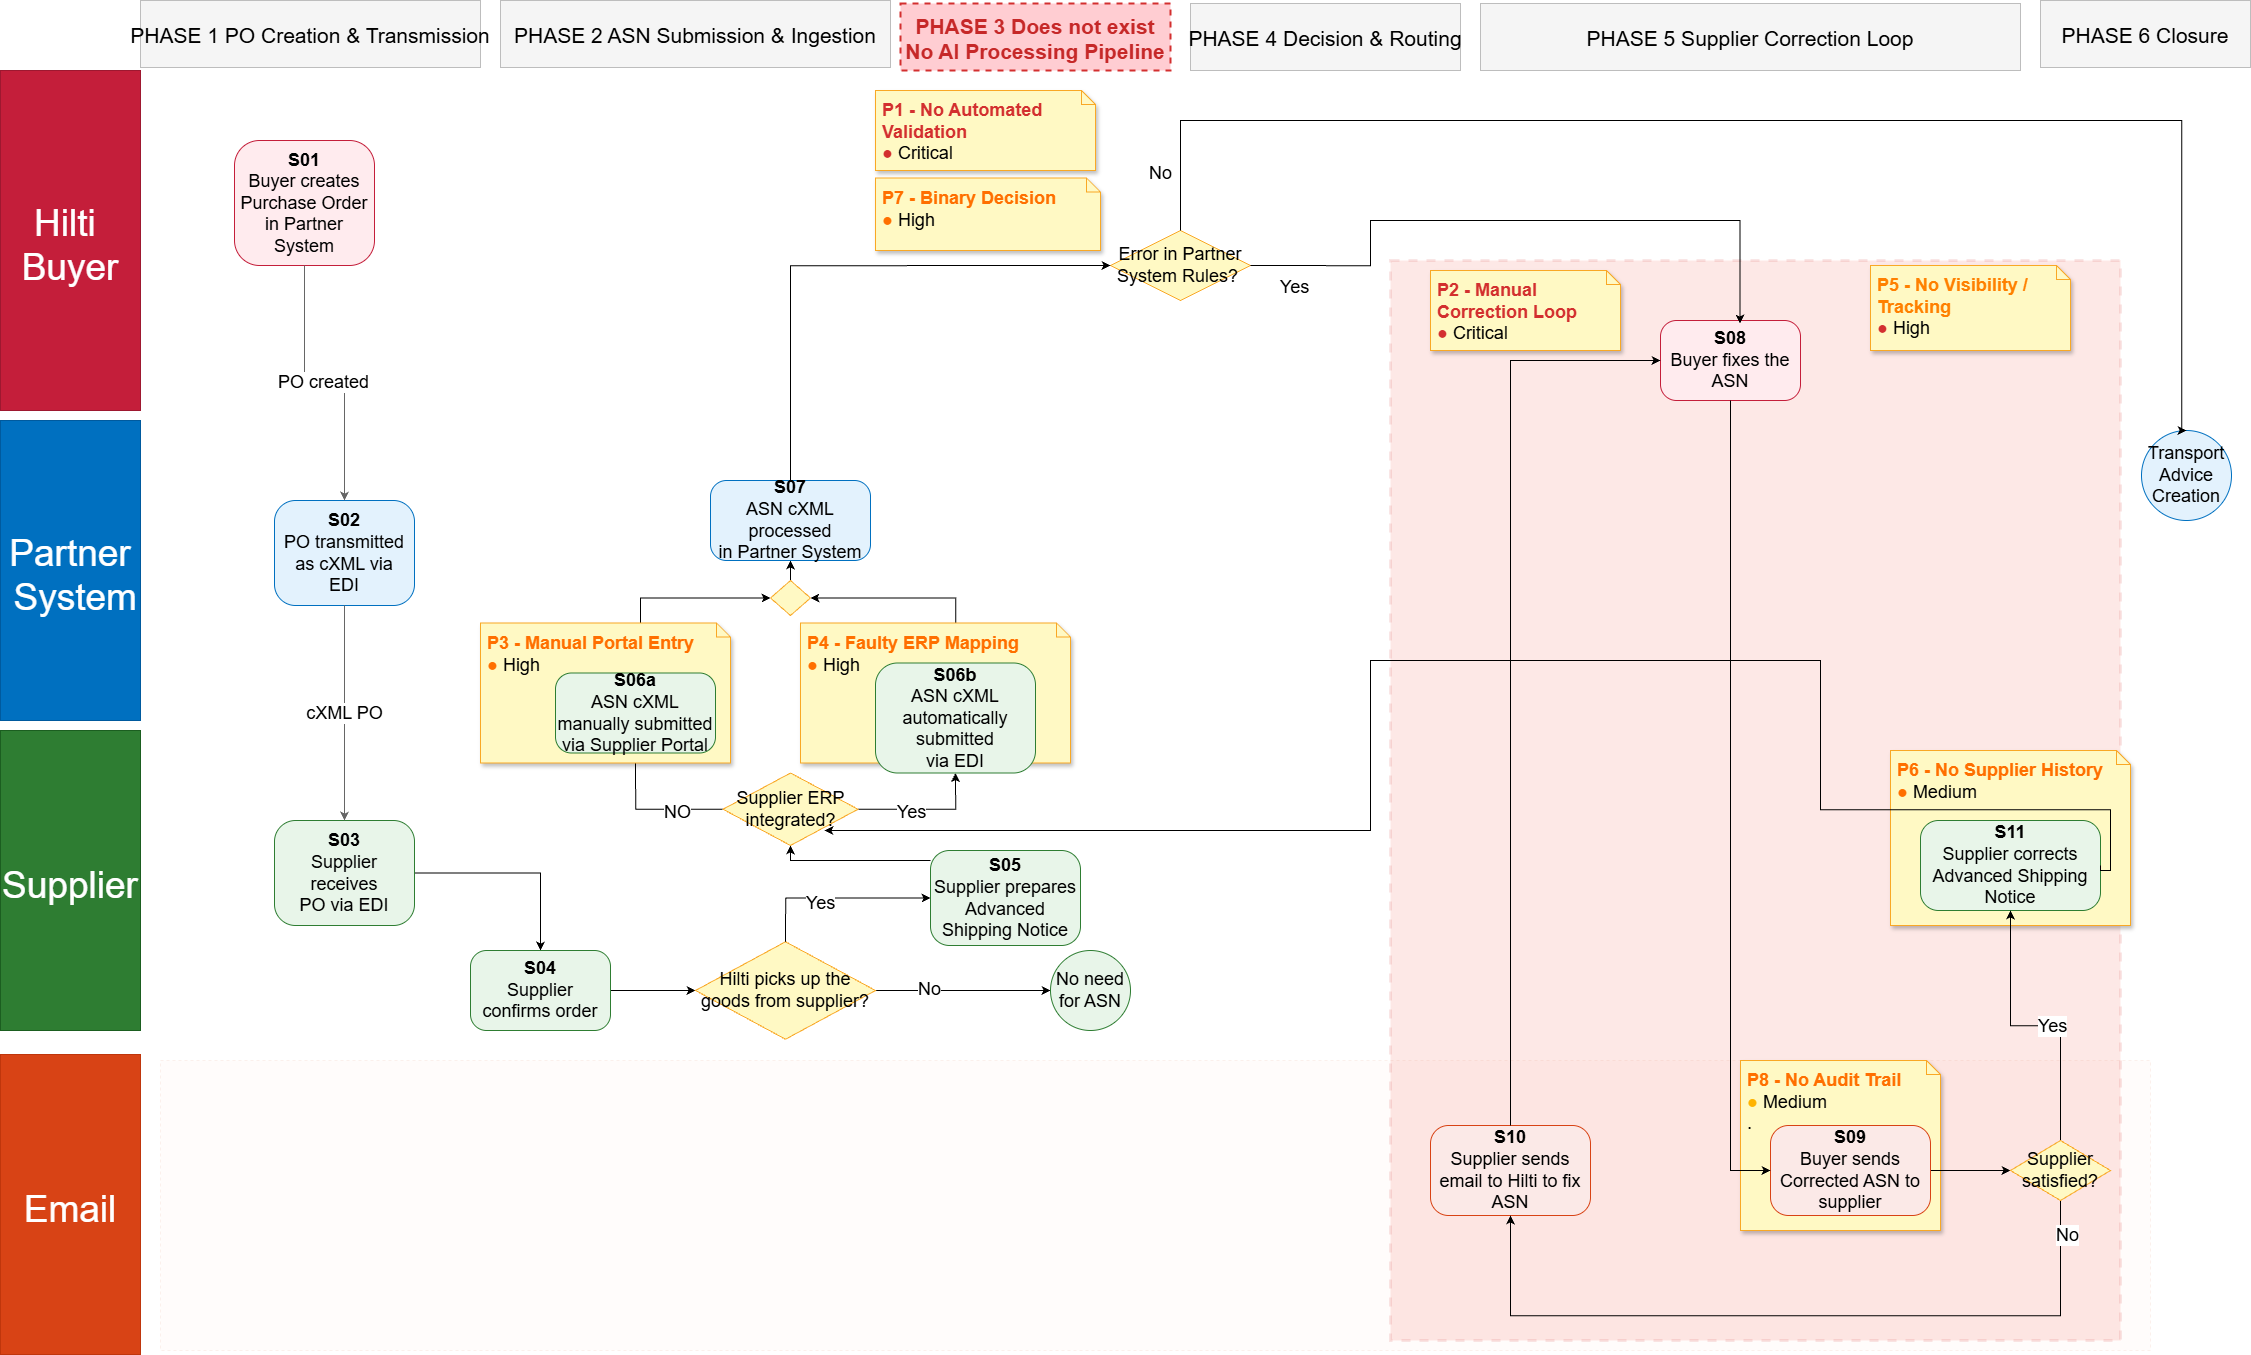
\includegraphics[width=\textwidth]{Figures/fig_4_A_asis_painpoints.png}
\caption{AS-IS process with pain points P1--P8 annotated.}
\label{fig:app:asis}
\end{figure}

The TO-BE process of Section~\ref{sec:emp:tobe} is reproduced below. Phase~3 (AI Processing Pipeline) is inserted between ASN submission and the partner's error check, and an audit log and a key performance indicator dashboard close the learning loop.

\begin{figure}[htbp]
\centering
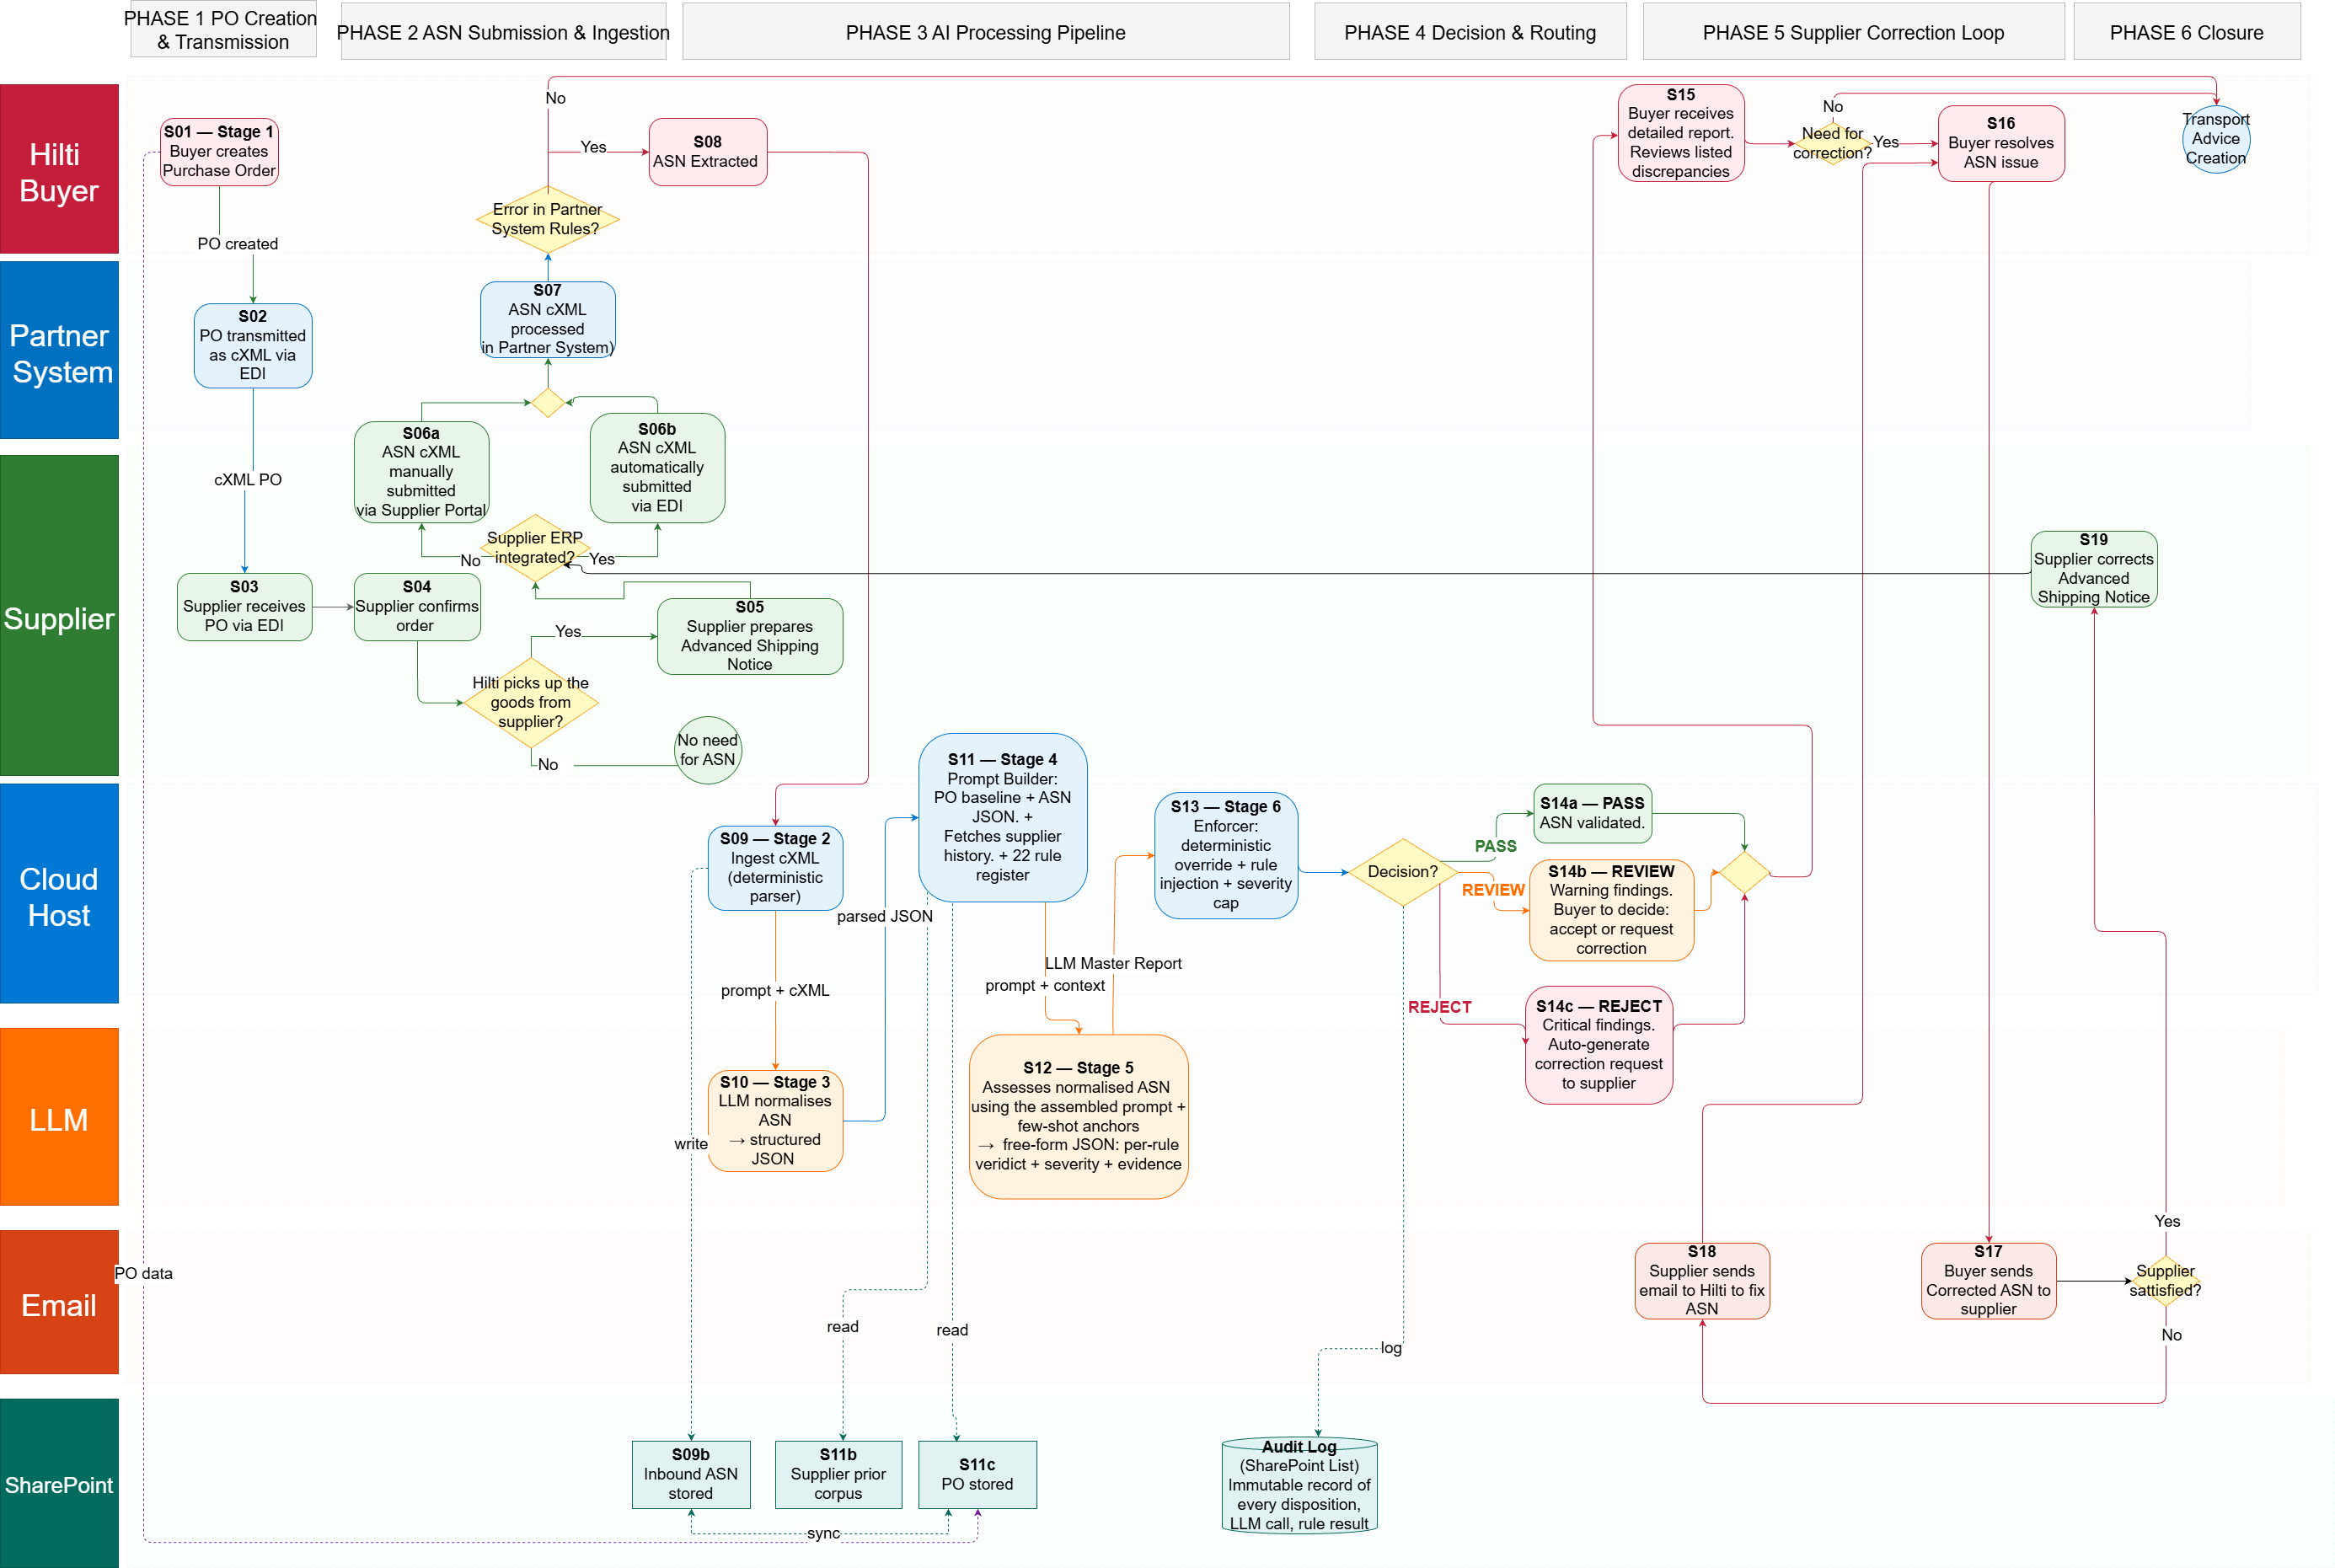
\includegraphics[width=\textwidth]{Figures/fig_4_2_tobe.png}
\caption{TO-BE validation process.}
\label{fig:emp:tobe}
\end{figure}


%% -----------------------------------------------------------------
%%  Appendix C --- Coverage of the rule register by partner static checks
%% -----------------------------------------------------------------
\chapter{Coverage of the rule register by the partner system's static checks} \label{app:emp:coverage}

This appendix maps every rule of the validation register R01--R22 against the static checks the partner system applies at receipt, supporting the claim in Section~\ref{sec:emp:asis} that the partner's coverage of the register is partial and the artefact's contribution is to close the residual gap.

\begin{table}[htbp]
\centering
\caption{Coverage of rules R01--R22 by the partner system's static checks.}
\label{tab:app:coverage}
\scriptsize
\begin{adjustbox}{max width=\textwidth}
\begin{tabular}{@{}lp{5cm}p{5cm}p{4.5cm}@{}}
\toprule
\textbf{Rule} & \textbf{What the rule asks} & \textbf{Covered by static check?} & \textbf{Where the pipeline adds} \\
\midrule
R01 & Quantity not over-shipped vs PO              & Partial --- row~7 catches overflow vs outstanding-to-notify & Severity calibration; REVIEW for partial overflow \\
R02 & Unit price matches PO                        & No                                                          & Pipeline only \\
R03 & Delivery date within tolerance               & Partial --- row~8 catches outside-window                    & REVIEW state for late-but-recoverable \\
R04 & Shipment date not before notice date         & No                                                          & Pipeline only \\
R05 & Unit-of-measure matches PO line              & No --- row~20 only checks dimension consistency             & Pipeline only (PO baseline match) \\
R06 & All PO lines present in ASN                  & No                                                          & Pipeline only \\
R07 & No phantom ASN lines                         & No                                                          & Pipeline only \\
R08 & Currency matches PO                          & No                                                          & Pipeline only \\
R09 & Supplier identity matches PO supplier        & No                                                          & Pipeline only \\
R10 & Each portion references a real PO            & Partial --- row~1 catches line number existence             & Pipeline catches portion-level mismatch \\
R11 & cXML schema compliance                       & Yes --- implicit XML schema validation                      & Recovered for symmetry; redundant on this rule \\
R12 & Mandatory delivery-date attribute present    & No --- row~8 only checks the value if present               & Pipeline catches absence \\
R13 & Transport terms match PO                     & No                                                          & Pipeline only \\
R14 & Ship-To address matches PO                   & No                                                          & Pipeline only \\
R15 & Line total = quantity $\times$ price         & No                                                          & Pipeline only \\
R16 & Partial shipment within tolerance            & Partial --- row~7 catches overflow only                     & Pipeline catches under threshold partials \\
R17 & Line is on the right PO portion              & No                                                          & Pipeline only \\
R18 & No duplicate shipment identifier             & Yes --- row~4                                               & Redundant on this rule \\
R19 & Shipment identifier within 35 characters     & Partial --- row~5, but silently                             & Pipeline catches it loudly, before submission \\
R20 & Gross-to-net weight ratio plausible          & Yes --- rows~11--12                                         & Redundant on this rule, with severity tier \\
R21 & Mandatory packaging block present            & Partial --- rows~16--19                                     & Redundant on this rule, with severity tier \\
R22 & Order not over-fulfilled cumulatively        & Partial --- row~3 catches ``fully shipped'' only            & Pipeline does cumulative shipped quantity tracking \\
\bottomrule
\end{tabular}
\end{adjustbox}
\end{table}

Of the 22 rules in the validation register, 3 (R11, R18 and R20) are fully covered by an existing static check at receipt; 7 (R01, R03, R10, R16, R19, R21 and R22) are partially covered, in the sense that the static check captures one corner of the rule but misses the calibration, the cumulative state, or the loud-versus-silent distinction; and 12 (R02, R04, R05, R06, R07, R08, R09, R12, R13, R14, R15 and R17) are not covered by any static check at all. The 12 uncovered rules are precisely those that compare the ASN against the PO baseline, depend on a supplier's prior history, or require a tiered REVIEW state, 3 classes of validation the partner system does not perform.


%% -----------------------------------------------------------------
%%  Appendix --- Ground truth labelling: checklist and annotation interface
%% -----------------------------------------------------------------
\chapter{Ground truth labelling: checklist and annotation interface} \label{app:emp:annotation}

This appendix details the labelling checklist of Section~\ref{sec:emp:protocol} and the purpose built annotation interface used to apply it, shown in Figure~\ref{fig:emp:annotation}.

\begin{figure}[htbp]
\centering
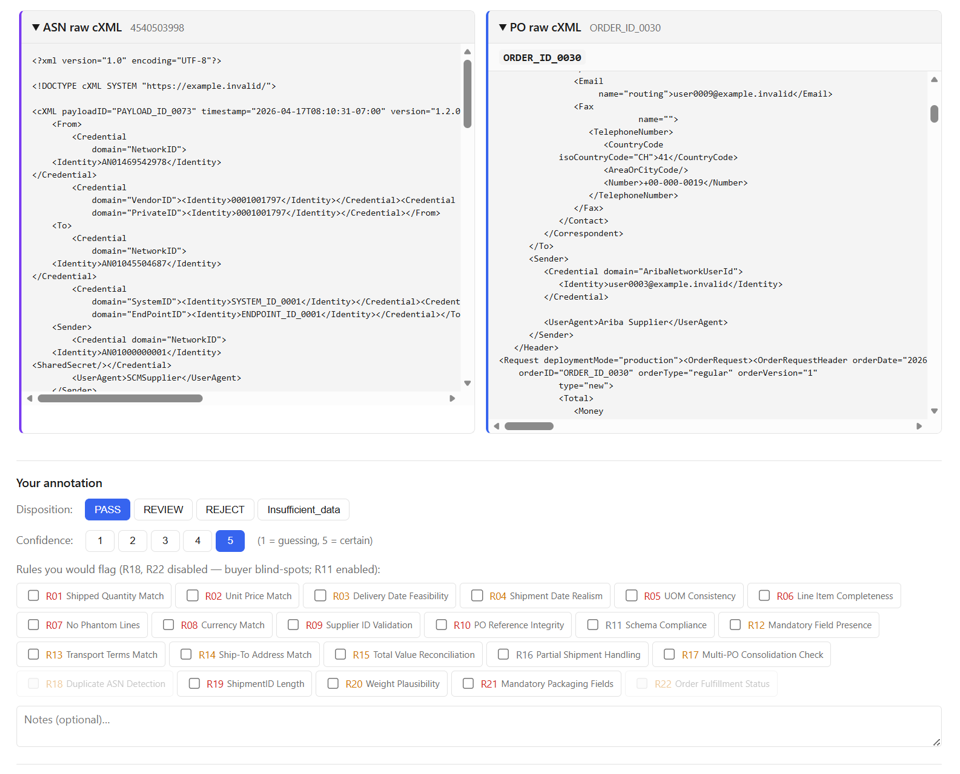
\includegraphics[width=\textwidth]{Figures/fig_D1_annotation.png}

\caption{Annotation interface used during ground truth labelling.}
\label{fig:emp:annotation}
\end{figure}

The interface in Figure~\ref{fig:emp:annotation} removes the per-case overhead the buyer team would otherwise carry: locating the cXML, retrieving the matching PO, opening both in a text editor and transcribing a disposition and a rule list into a spreadsheet. It collapses those steps into a single screen and constrains the analyst to the verdicts the protocol admits. Each case loads with the ASN cXML and the matching PO cXML side by side, both in their raw form, so that the analyst remains close to the document of record and to the evidence the rule register evaluates against.

The annotation panel exposes 4 controls. A disposition selector records the case-level verdict (PASS, REVIEW or REJECT). A 5-point confidence selector records how certain the analyst is of the disposition, on a scale anchored at 1 (guessing) and 5 (certain), and is retained as an audit covariate rather than entering the agreement statistics of Section~\ref{sec:method:eval}. A per rule checklist lets the analyst flag the rules that justify the disposition. A free text notes field captures rationale or edge-case observations that the rule checklist cannot accommodate, and is the source of the failure cluster reasoning in Section~\ref{sec:emp:clustering}.

For every ASN, each analyst labels the rules the checklist exposes as PASS, FAIL or N/A. Two rules are prefilled N/A because neither can be answered from a single ASN card, which leaves 20 rules for the analyst to verdict. R22 (order fulfilment) needs the cumulative shipped quantity across earlier ASNs for the same PO line, and R11 (cXML schema compliance) is an ingestion-time entry check, so a schema-invalid ASN is rejected before it reaches the worksheet and R11 has already passed on every case the analyst sees. R11 and R22 are disabled in the checklist, matching this pre-fill so that the analyst is structurally prevented from labelling cells the protocol cannot answer.

The rules prefilled N/A in labelling are not the same exclusion as the per rule recall denominator of Chapter~\ref{chap:results}. Labelling sets R11 and R22 aside; the recall denominator instead sets R11 and R18 aside, leaving 20 evaluable rules, because R18 (duplicate detection) is exercised by a separate re-submission check rather than by a single ASN verdict. The 2 exclusions are built for different purposes and coincide only on R11.


%% -----------------------------------------------------------------
%%  Appendix E --- Supporting tables for Sections 4.5.4 and 4.5.5
%% -----------------------------------------------------------------
\chapter{Supporting tables for the supplier prior and the real world ground truth} \label{app:emp:supporting}

This appendix gathers the supporting tables for the evaluation set. Table~\ref{tab:emp:blocks} summarises the 3 blocks; Table~\ref{tab:app:percase} lists the buyer ground truth for every real world case in Blocks~A and~B; and Table~\ref{tab:app:perrule} reports the per rule fail rate underlying the prompt sentences of Table~\ref{tab:emp:prompts}.

\begin{table}[htbp]
\centering
\caption{Block summary by source, scope, structural shape and disposition (PASS / REVIEW / REJECT). Referenced from Section~\ref{sec:emp:sources}.}
\label{tab:emp:blocks}
\small
\renewcommand{\arraystretch}{1.3}
\begin{adjustbox}{max width=\textwidth}
\begin{tabular}{@{}llp{3.6cm}rrrc@{}}
\toprule
\textbf{Block} & \textbf{Source} & \textbf{Case range} & \textbf{\# ASNs} & \textbf{\# POs} & \textbf{Multi-PO} & \textbf{Disposition mix} \\
\midrule
A. Production       & Partner platform tracker                  & P-26 to P-61$^{*}$            & 28 & 34  & 3 (11\,\%)  & 4 / 11 / 13 \\
B. Pre-integration  & Same tracker (onboarding flow)            & PI-01 to PI-04                & 4  & 17  & 3 (75\,\%)  & 0 / 4 / 0 \\
C. Synthetic        & Deterministic mutation of clean templates & S-01--S-51, SYN-M01--M17 & 68 & 112 & 11 (16\,\%) & 10 / 23 / 35 \\
\midrule
\textbf{Total} & --- & --- & \textbf{100} & \textbf{163} & \textbf{17 (17\,\%)} & \textbf{14 / 38 / 48} \\
\bottomrule
\end{tabular}
\end{adjustbox}
\par\vspace{0.2em}\footnotesize{$^{*}$ Non-contiguous; gaps are cases removed by the inclusion filter.}
\end{table}

Block~C is summarised here at its full size of 68 cases. One case, S-18 (rule R18, duplicate detection), is tested by a separate re-submission check rather than by a static cXML edit, so it carries no static disposition. The Block~C disposition metrics in Chapter~\ref{chap:results} are therefore reported on the remaining 67 cases.

\begin{table}[htbp]
\centering
\caption{Per-case buyer ground truth on the production and pre-integration sample (32 cases: 4~PASS, 15~REVIEW, 13~REJECT).}
\label{tab:app:percase}
\scriptsize
\begin{adjustbox}{max width=\textwidth}
\begin{tabular}{@{}lllp{2.4cm}p{5.5cm}p{3cm}@{}}
\toprule
\textbf{Case} & \textbf{Block} & \textbf{Supplier} & \textbf{Buyer disposition} & \textbf{Rules flagged} & \textbf{Notes} \\
\midrule
P-26  & A & S2 (CH)  & REJECT  & R02, R08, R13, R14                                  & \\
P-27  & A & S2 (CH)  & REJECT  & R02, R08, R13, R14                                  & \\
P-28  & A & S3 (CH)  & PASS    & ---                                                 & \\
P-29  & A & S3 (CH)  & PASS    & ---                                                 & Timestamp \\
P-30  & A & S3 (CH)  & PASS    & ---                                                 & Timestamp \\
P-31  & A & S5 (US)  & REVIEW  & R03                                                 & Timestamp \\
P-32  & A & S6 (DE)  & PASS    & ---                                                 & Timestamp \\
P-33  & A & S7 (CH)  & REVIEW  & R21 & Timestamp; Multi-PO (3 POs) \\
P-34  & A & S4 (CN)  & REVIEW  & R21                                                 & Timestamp \\
P-35  & A & S4 (CN)  & REVIEW  & R21 & Timestamp; Multi-PO (2 POs) \\
P-36  & A & S1 (AT)  & REJECT  & R02, R05, R08, R13, R14                             & \\
P-37  & A & S1 (AT)  & REJECT  & R13, R14                                            & \\
P-38  & A & S1 (AT)  & REJECT  & R02, R06, R12, R14, R21                             & \\
P-39  & A & S1 (AT)  & REJECT  & R02, R06, R12, R13, R14                             & \\
P-40  & A & S1 (AT)  & REJECT  & R02, R06, R12, R13, R14                             & \\
P-41  & A & S1 (AT)  & REJECT  & R06, R12, R13, R14                                  & \\
P-42  & A & S1 (AT)  & REJECT  & R02, R05, R06, R08, R12, R13, R14                   & \\
P-43  & A & S1 (AT)  & REJECT  & R02, R05, R06, R08, R12, R13, R14                   & \\
P-44  & A & S1 (AT)  & REJECT  & R08, R14, R21                                       & \\
P-45  & A & S12 (CZ) & REVIEW  & R03, R06, R13, R14, R21 & \\
P-48  & A & S12 (CZ) & REVIEW  & R03, R06, R13, R14, R21 & Multi-PO (4 POs) \\
P-51  & A & S13 (CH) & REJECT  & R03, R08, R13, R14, R21                             & \\
P-54  & A & S17 (CH) & REVIEW  & R03, R13, R14, R21                                  & \\
P-55  & A & S18 (HU) & REVIEW  & R13, R14, R21                                       & \\
P-57  & A & S19 (CH) & REVIEW  & R03, R06, R13, R14, R21                             & \\
P-58  & A & S20 (IT) & REVIEW  & R03, R13, R14, R21                                  & \\
P-59  & A & S20 (IT) & REJECT  & R08, R13, R14, R21                                  & \\
P-61  & A & S21 (DE) & REVIEW  & R13, R14, R21                                       & \\
PI-01 & B & S8 (GB)  & REVIEW  & R03, R13, R14, R21                                  & Multi-PO (8 POs) \\
PI-02 & B & S9 (AT)  & REVIEW  & R13, R14, R21                                       & Multi-PO (3 POs) \\
PI-03 & B & S10 (BE) & REVIEW  & R13, R14, R21                                       & Single-PO \\
PI-04 & B & S11 (DE) & REVIEW  & R03, R06, R13, R14, R21                             & Multi-PO (5 POs) \\
\bottomrule
\end{tabular}
\end{adjustbox}
\end{table}

\begin{table}[htbp]
\centering
\caption{Per rule fail rate by supplier on the prior corpus. Cells are blank where no firing was recorded; only the 8 rules active in the corpus are shown.}
\label{tab:app:perrule}
\footnotesize
\begin{adjustbox}{max width=\textwidth}
\begin{tabular}{@{}lcccccccc@{}}
\toprule
\textbf{Supplier} & \textbf{R02} & \textbf{R03} & \textbf{R06} & \textbf{R08} & \textbf{R12} & \textbf{R13} & \textbf{R14} & \textbf{R21} \\
\midrule
S1 (AT)  & 0.67 & ---  & 0.67 & 0.44 & 0.67 & 0.78 & 1.00 & 0.22 \\
S2 (CH)  & 1.00 & ---  & ---  & 1.00 & ---  & 1.00 & 1.00 & ---  \\
S3 (CH)  & ---  & ---  & ---  & ---  & ---  & ---  & ---  & ---  \\
S4 (CN)  & ---  & ---  & ---  & ---  & ---  & ---  & ---  & ---  \\
S12 (CZ) & ---  & 1.00 & 1.00 & ---  & ---  & 1.00 & 1.00 & 1.00 \\
\bottomrule
\end{tabular}
\end{adjustbox}
\end{table}

\begin{table}[htbp]
\centering
\caption{The 5 supplier prompt lines. Sentences are shown for the full corpus, after the pipeline's evaluation sweep.}
\label{tab:emp:prompts}
\scriptsize
\begin{adjustbox}{max width=\textwidth}
\begin{tabular}{@{}llp{8.2cm}p{4.2cm}@{}}
\toprule
\textbf{Supplier} & \textbf{Prior} & \textbf{Prompt sentence} & \textbf{Intent} \\
\midrule
S1 (AT) & REJECT &
``Historical note: this supplier has failed R14 in 9/9, R13 in 7/9, R02 in 6/9 prior ASN(s). Pay extra attention to those checks.'' &
Lean toward REJECT on address, transport and price. \\
\addlinespace
S2 (CH) & REJECT &
``Historical note: this supplier has failed R02 in 2/2, R08 in 2/2, R13 in 2/2 prior ASN(s). Pay extra attention to those checks.'' &
Lean toward REJECT on price, currency and transport. \\
\addlinespace
S3 (CH) & PASS &
``Historical note: the buyer has validated all 3 prior ASN(s) from this supplier as PASS (zero rule failures recorded). Note: 2/3 prior ASN(s) failed upstream in SAP due to a known order confirmation timestamp bug, and those should pass under current rules; do not let the historical failure count inflate REVIEW/REJECT signals for this supplier on similar cases.'' &
Ignore the visible failure history; it is a platform artefact. \\
\addlinespace
S4 (CN) & REVIEW &
``Historical note: this supplier has 2 prior ASN(s) on file, both REVIEW (R21 missing packaging). The prior failures coincide with a known order-confirmation timestamp bug in SAP; weigh content-level evidence above the timestamp signal.'' &
Read R21 as the genuine signal; do not over-attribute to the platform artefact. \\
\addlinespace
S12 (CZ) & REVIEW &
``Historical note: this supplier has failed R03 in 2/2, R06 in 2/2, R13 in 2/2 prior ASN(s). Pay extra attention to those checks.'' &
Watch delivery date, partial delivery and transport. \\
\bottomrule
\end{tabular}
\end{adjustbox}
\end{table}


\clearpage
\section*{Full synthetic perturbation inventory (S-01 to S-51)}

Table~\ref{tab:app:mutants_full} enumerates the 51 single rule synthetic mutants of Block~C, reported per case with target rule, design group, expected disposition, collateral rules and the cXML edit applied. Mutants S-01 to S-22 each target a single rule across the register R01 to R22; mutants S-23 to S-51 extend the block along the three design groups introduced in Section~\ref{sec:emp:synthetic}: boundary, magnitude and mechanism, and supplier diversity.

\footnotesize
\begin{longtable}{@{}llllp{6.5cm}@{}}
\caption{Full synthetic perturbation inventory: S-01 to S-51 single rule mutants.}\label{tab:app:mutants_full}\\
\toprule
\textbf{Case} & \textbf{Target} & \textbf{Group} & \textbf{Expected} & \textbf{cXML edit applied} \\
\midrule
\endfirsthead
\toprule
\textbf{Case} & \textbf{Target} & \textbf{Group} & \textbf{Expected} & \textbf{cXML edit applied} \\
\midrule
\endhead
\midrule
\multicolumn{5}{r}{\emph{Continued on next page}} \\
\endfoot
\bottomrule
\endlastfoot
S-01 & R01 & Base & REJECT & Quantity 2016 $\to$ 3000 (49\,\% over-fulfilment, 0\,\% tolerance) \\
S-02 & R02 & Base & REJECT & Unit price 2.26 $\to$ 5.00 \\
S-03 & R03 & Base & REVIEW & Delivery date 49 days late \\
S-04 & R04 & Base & REVIEW & Shipment date set before notice date \\
S-05 & R05 & Base & REJECT & UOM H87 $\to$ KGM (PO expects H87) \\
S-06 & R06 & Base & REVIEW & Removed ShipNoticeItem line=10 \\
S-07 & R07 & Base & REJECT & Phantom ShipNoticeItem line=99 \\
S-08 & R08 & Base & REJECT & Currency EUR $\to$ USD \\
S-09 & R09 & Base & REJECT & Supplier NetworkID 0014 $\to$ 0015 \\
S-10 & R10 & Base & REJECT & Added second portion against non-existent PO \\
S-11 & ---  & Base (PASS) & PASS & Clean ASN, schema valid (R11 PASS control) \\
S-12 & R12 & Base & REVIEW & Removed deliveryDate attribute \\
S-13 & R13 & Base & REVIEW & Transport terms FCA $\to$ DDP \\
S-14 & R14 & Base & REVIEW & Ship-To addressID 0524 $\to$ 9999 \\
S-15 & R15 & Base & REJECT & Line total inconsistent with quantity $\times$ price \\
S-16 & R16 & Base & REVIEW & Quantity 2016 $\to$ 1000 (50\,\% partial shipment) \\
S-17 & R17 & Base & REVIEW & Line moved to wrong PO portion \\
S-18$^{\dagger}$ & R18 & Base (nominal) & REVIEW & Duplicate shipment identifier check (sequential re-submission, not a static edit) \\
S-19 & R19 & Base & REJECT & Shipment identifier 42 characters (limit 35) \\
S-20 & R20 & Base & REVIEW & Gross / net weight ratio above $100\times$ \\
S-21 & R21 & Base & REJECT & Removed all packaging dimensions \\
S-22 & R22 & Base & REJECT & Quantity 2016 $\to$ 4032 (2$\times$ PO quantity) \\
\midrule
S-23 & --- & Boundary (PASS) & PASS  & Just inside PASS control \\
S-24 & --- & Boundary (PASS) & PASS  & Just inside PASS control \\
S-25 & --- & Boundary (PASS) & PASS  & Just inside PASS control (R20 ratio exactly at 10.0) \\
S-26 & --- & Boundary (PASS) & PASS  & Just inside PASS control \\
S-27 & --- & Boundary (PASS) & PASS  & Just inside PASS control \\
S-28 & --- & Boundary (PASS) & PASS  & Just inside PASS control \\
S-29 & R03 & Boundary        & REVIEW & R03 delivery window edge case \\
S-30 & R03 & Boundary        & REVIEW & R03 delivery window edge case \\
S-31 & R19 & Boundary        & REJECT & R19 35 character limit edge case \\
S-32 & R20 & Boundary        & REVIEW & R20 weight ratio edge case \\
S-33 & R01 & Boundary        & REJECT & R01 zero tolerance tightest margin \\
S-34 & R02 & Boundary        & REJECT & R02 zero tolerance tightest margin \\
\midrule
S-35 & R16 & Magnitude/mechanism        & REVIEW & R16 partial shipment, alternative magnitude \\
S-36 & R02 & Magnitude/mechanism        & REJECT & R02 under pricing variant \\
S-37 & R05 & Magnitude/mechanism (PASS) & PASS   & R05 canonical equivalent UOM (PASS control) \\
S-38 & R06 & Magnitude/mechanism        & REJECT & R06 full-miss critical variant \\
S-39 & R08 & Magnitude/mechanism        & REJECT & R08 line-level currency mismatch \\
S-40 & R09 & Magnitude/mechanism (PASS) & PASS   & R09 VendorID only (PASS control) \\
S-41 & R13 & Magnitude/mechanism        & REVIEW & R13 \texttt{value="Other"} text path \\
S-42 & R21 & Magnitude/mechanism        & REVIEW & R21 net-only missing dimension variant \\
S-43 & R21 & Magnitude/mechanism        & REVIEW & R21 type only missing dimension variant \\
S-44 & R12 & Magnitude/mechanism        & REVIEW & R12 missing line number variant \\
\midrule
S-45 & R08 & Supplier diversity (template C)   & REJECT & R08 currency mismatch on template C \\
S-46 & R02 & Supplier diversity (template C)   & REJECT & R02 unit price mismatch on template C \\
S-47 & R03 & Supplier diversity (template C)   & REVIEW & R03 late delivery on template C \\
S-48 & R21 & Supplier diversity (template C)   & REVIEW & R21 missing packaging on template C \\
S-49 & R02 & Supplier diversity (template D) & REJECT & R02 unit price mismatch on template D \\
S-50 & R08 & Supplier diversity (template D) & REJECT & R08 currency mismatch on template D \\
S-51 & R03 & Supplier diversity (template D) & REVIEW & R03 late delivery on template D \\
\end{longtable}
\par\vspace{0.2em}\footnotesize{$^{\dagger}$ Tested by a separate re-submission check, not a static cXML edit; excluded from the Chapter~\ref{chap:results} disposition cohort.}
\normalsize

\begin{table}[htbp]
\centering
\caption{Multi-rule synthetic scenarios (Block~C, multi-rule subset, SYN-M01 to SYN-M17).}
\label{tab:app:multirule}
\footnotesize
\begin{adjustbox}{max width=\textwidth}
\begin{tabular}{@{}lp{6.5cm}ll@{}}
\toprule
\textbf{Case} & \textbf{Combined defects} & \textbf{Target rules} & \textbf{Expected} \\
\midrule
SYN-M01 & Over-shipment + currency mismatch + missing packaging                & R01, R08, R21   & REJECT \\
SYN-M02 & Late delivery + UOM mismatch + wrong supplier identifier             & R03, R05, R09   & REJECT \\
SYN-M03 & Unit price mismatch + phantom ASN line                               & R02, R07        & REJECT \\
SYN-M04 & Partial shipment + wrong transport terms                             & R13, R16        & REVIEW \\
SYN-M05 & Line total inconsistency + over length shipment ID + missing packaging & R15, R19, R21 & REJECT \\
SYN-M06 & Quantity over shipment + line total inconsistency                    & R01, R15        & REJECT \\
SYN-M07 & Quantity over shipment + currency mismatch                           & R01, R08        & REJECT \\
SYN-M08 & Phantom ASN line + wrong transport terms                             & R07, R13        & REJECT \\
SYN-M09 & Quantity + unit price + line total errors compounded                 & R01, R02, R15   & REJECT \\
SYN-M10 & Partial shipment + missing packaging                                 & R16, R21        & REJECT \\
SYN-M11 & Currency mismatch + wrong transport terms                            & R08, R13        & REJECT \\
SYN-M12 & Late delivery + wrong transport terms                                & R03, R13        & REVIEW \\
SYN-M13 & Multi-rule PASS control (no defects)                                 & ---             & PASS   \\
SYN-M14 & UOM mismatch + partial shipment                                      & R05, R16        & REJECT \\
SYN-M15 & Currency mismatch + over length shipment ID + missing packaging      & R08, R19, R21   & REJECT \\
SYN-M16 & Unit price mismatch + wrong supplier identifier                      & R02, R09        & REJECT \\
SYN-M17 & Quantity over shipment + late delivery + wrong transport terms       & R01, R03, R13   & REJECT \\
\bottomrule
\end{tabular}
\end{adjustbox}
\end{table}


\chapter{Operational measurements}
\label{app:operational}

This appendix reports the full operational spread per pipeline design on the 28 production evaluation cases per design. The headline figures, median latency and mean cost per ASN, are cited in Chapter~\ref{chap:results}, Section~\ref{sec:results:cost}; the full descriptive spread is reported here.

\begin{table}[htbp]
\centering
\caption{Operational spread per design on the 28 production evaluation cases per design. Costs are in euros. Q1 and Q3 are the lower and upper quartiles; p90 and p95 are the values below which 90\% and 95\% of cases fall. The 99th percentile is omitted because with 28 cases it collapses onto the maximum.}
\label{tab:app:operational}
\footnotesize
\setlength{\tabcolsep}{4pt}

\begin{adjustbox}{max width=\textwidth}
\begin{tabular}{@{}lrrrrrrrr@{}}
\multicolumn{9}{l}{\textbf{Latency per ASN (seconds)}} \\
\toprule
\textbf{Design} & \textbf{Min} & \textbf{Q1} & \textbf{Median} & \textbf{Q3} & \textbf{p90} & \textbf{p95} & \textbf{Max} & \textbf{StdDev} \\
\midrule
pure LLM      & 10.65 & 11.88 & 13.14 & 15.74 & 20.00 & 32.30 & 34.98 & 5.70 \\
post hoc      & 10.58 & 12.13 & 13.94 & 16.19 & 21.77 & 30.09 & 36.22 & 5.81 \\
LLM-as-judge  & 12.04 & 12.85 & 13.67 & 16.72 & 23.24 & 35.19 & 38.33 & 7.04 \\
in generation & 9.10  & 11.37 & 13.22 & 16.94 & 23.22 & 33.81 & 48.47 & 7.93 \\
pre hoc       & 7.05  & 7.48  & 7.89  & 9.45  & 10.11 & 12.27 & 15.38 & 1.73 \\
\bottomrule
\end{tabular}
\end{adjustbox}

\medskip

\begin{adjustbox}{max width=\textwidth}
\begin{tabular}{@{}lrrrrrr@{}}
\multicolumn{7}{l}{\textbf{Tokens and cost per ASN}} \\
\toprule
\textbf{Design} & \textbf{Prompt mean} & \textbf{Completion mean} & \textbf{Cost mean (EUR)} & \textbf{Cost p95} & \textbf{Cost max} & \textbf{Cost StdDev} \\
\midrule
pure LLM      & 12{,}615 & 3{,}723 & 0.109 & 0.201 & 0.500 & 0.080 \\
post hoc      & 12{,}614 & 3{,}838 & 0.111 & 0.203 & 0.502 & 0.081 \\
LLM-as-judge  & 15{,}859 & 3{,}931 & 0.127 & 0.247 & 0.518 & 0.086 \\
in generation & 26{,}244 & 3{,}662 & 0.171 & 0.351 & 0.563 & 0.100 \\
pre hoc       & 9{,}870  & 1{,}970 & 0.073 & 0.111 & 0.463 & 0.075 \\
\bottomrule
\end{tabular}
\end{adjustbox}
\end{table}

\paragraph{Annual volume basis for the cost projection.} The cost projection in Section~\ref{sec:results:cost} scales the per-case handling time by the live ASN volume. In a representative month of live production the function processed 2,331 unique ASNs, of which 51 failed validation, a fail rate of about 2 per cent; this is of the order of 28,000 ASNs and 610 failed ASNs per year. Each failed ASN triggers the 30 to 90 minute correction loop, and 2 factors raise the per-case time above a single document handled by one buyer. First, the buyer opens and compares the ASN against each PO it references, so the time scales with the number of documents handled; the production sample averages 1.48 referenced POs per ASN, with 21 per cent referencing more than one, so an average case handles about 2.48 documents against 2 for a single-PO case, a measured uplift of about a quarter (a factor of 1.24). Second, a buyer without spare capacity escalates a case to colleagues, so a case is sometimes worked by more than one buyer; no escalation rate is recorded, so a conservative factor of 1.5 is assumed and is flagged as an assumption rather than a measurement. Applying both factors to the 610 failed ASNs per year at 30 to 90 minutes each gives of the order of 570 to 1,700 analyst hours per year.

\paragraph{Hourly cost basis for the labour saving estimate.} The labour saving in Section~\ref{sec:concl:practice} values the analyst hours removed at the loaded hourly cost of a materials manager at the partner organisation, about EUR 38 per hour. This is derived from an annual salary of roughly EUR 82,000, spread over 13 payments, 4 working weeks per month and 41.75 working hours per week. Multiplying the estimated 570 to 1,700 analyst hours per year by this rate gives the order of EUR 22,000 to 65,000 per year.

\begin{figure}[htb]
\centering
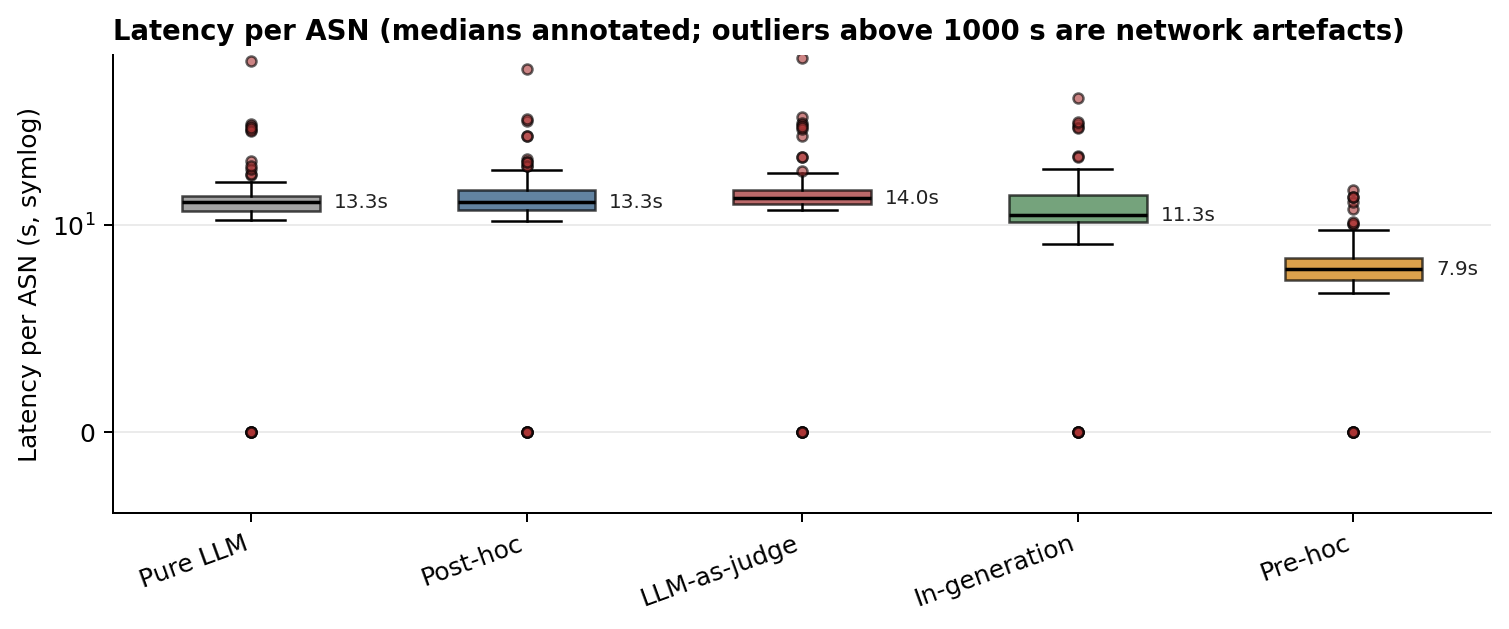
\includegraphics[width=0.82\textwidth]{Figures/fig_5_5_latency_box.png}
\caption{Latency per ASN by design (box = interquartile range, line = median, points = provider-delay outliers). Referenced from Section~\ref{sec:results:cost}.}
\label{fig:results:latency}
\end{figure}

\begin{figure}[htb]
\centering
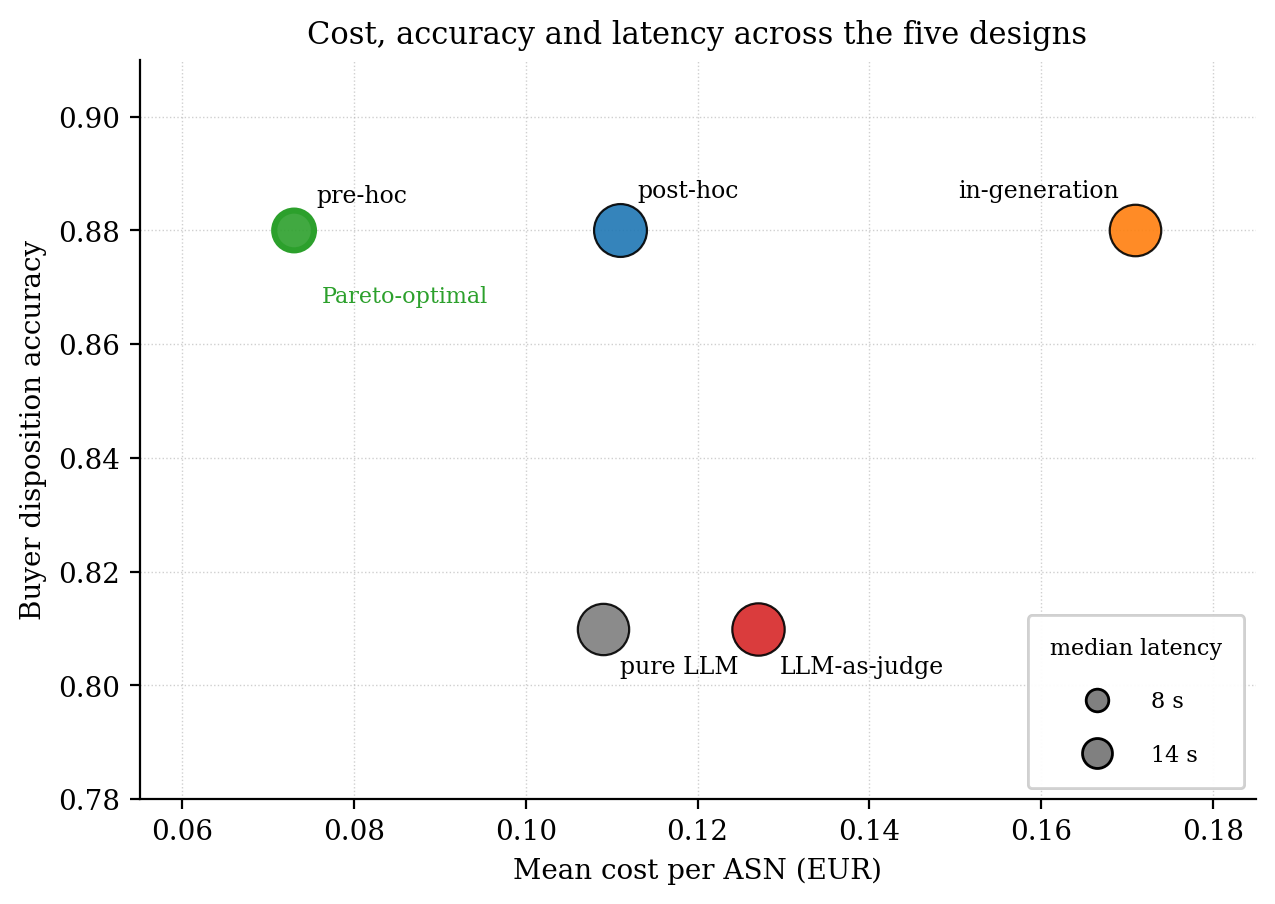
\includegraphics[width=0.78\textwidth]{Figures/fig_5_pareto.png}
\caption{Cost and latency on the 28 production cases and accuracy on the 32 buyer cases; marker area is median latency. Referenced from Section~\ref{sec:results:cost}.}
\label{fig:results:pareto}
\end{figure}


%% -----------------------------------------------------------------
%%  Appendix: Full disposition metrics (Chapter 5)
%% -----------------------------------------------------------------
\chapter{Full disposition metrics}
\label{app:dispmetrics}

This appendix reports the point estimates and 95 per cent bootstrap confidence intervals for all 4 disposition metrics, on both samples. The bar chart of Figure~\ref{fig:results:metrics} in Chapter~\ref{chap:results} summarises these values; the full table is given here.

\begin{table}[htbp]
\centering
\caption{Disposition agreement and per rule recall on the synthetic cohort (67 cases). 95 per cent bootstrap intervals in brackets; recall is over the 41 evaluable single rule mutant targets.}
\label{tab:app:dispsynth}
\footnotesize
\begin{adjustbox}{max width=\textwidth}
\begin{tabular}{@{}lccccc@{}}
\toprule
\textbf{Design} & \textbf{Accuracy} & \textbf{Weighted F1} & \textbf{Weighted kappa} & \textbf{Gwet AC2} & \textbf{Rule recall} \\
\midrule
pure LLM      & 0.81 [0.70, 0.90] & 0.80 [0.70, 0.89] & 0.78 [0.63, 0.90]        & 0.79 [0.68, 0.90] & 29/41 = 0.71 \\
post hoc      & 0.87 [0.78, 0.94] & 0.87 [0.78, 0.94] & 0.86 [0.77, 0.94]        & 0.87 [0.78, 0.94] & 37/41 = 0.90 \\
LLM-as-judge  & 0.51 [0.37, 0.64] & 0.42 [0.28, 0.57] & $-$0.01 [$-$0.12, 0.13]  & 0.49 [0.30, 0.65] & 26/41 = 0.63 \\
in generation & 0.84 [0.75, 0.91] & 0.84 [0.75, 0.91] & 0.80 [0.65, 0.91]        & 0.82 [0.71, 0.92] & 28/41 = 0.68 \\
pre hoc       & 0.88 [0.79, 0.96] & 0.88 [0.79, 0.95] & 0.88 [0.79, 0.95]        & 0.88 [0.80, 0.95] & 40/41 = 0.98 \\
\bottomrule
\end{tabular}
\end{adjustbox}
\end{table}

\begin{table}[htbp]
\centering
\caption{Disposition agreement and per rule recall on the buyer sample (32 cases, 28 production and 4 pre-integration). 95 per cent bootstrap intervals in brackets.}
\label{tab:app:dispbuyer}
\footnotesize
\begin{adjustbox}{max width=\textwidth}
\begin{tabular}{@{}lccccc@{}}
\toprule
\textbf{Design} & \textbf{Accuracy} & \textbf{Weighted F1} & \textbf{Weighted kappa} & \textbf{Gwet AC2} & \textbf{Rule recall} \\
\midrule
pure LLM      & 0.81 [0.66, 0.94] & 0.80 [0.64, 0.94] & 0.78 [0.58, 0.93] & 0.82 [0.68, 0.94] & 40/106 = 0.38 \\
post hoc      & 0.88 [0.75, 0.97] & 0.82 [0.65, 0.95] & 0.82 [0.69, 0.94] & 0.88 [0.75, 0.97] & 55/106 = 0.52 \\
LLM-as-judge  & 0.81 [0.66, 0.94] & 0.76 [0.58, 0.92] & 0.75 [0.60, 0.89] & 0.83 [0.68, 0.95] & 43/106 = 0.41 \\
in generation & 0.88 [0.75, 0.97] & 0.82 [0.65, 0.95] & 0.82 [0.69, 0.94] & 0.88 [0.75, 0.97] & 43/106 = 0.41 \\
pre hoc       & 0.88 [0.75, 0.97] & 0.82 [0.65, 0.95] & 0.82 [0.69, 0.94] & 0.88 [0.75, 0.97] & 51/106 = 0.48 \\
\bottomrule
\end{tabular}
\end{adjustbox}
\end{table}

\begin{table}[htbp]
\centering
\caption{Severity-weighted macro F1 by rule regime (fail = positive class; severity weights 1/2/3). Parentheses give the contributing rules. Referenced from Section~\ref{sec:results:regimes}.}
\label{tab:results:fwslices}
\footnotesize
\begin{adjustbox}{max width=\textwidth}
\begin{tabular}{@{}lcccccc@{}}
\toprule
& \multicolumn{3}{c}{\textbf{Synthetic}} & \multicolumn{3}{c}{\textbf{Buyer}} \\
\cmidrule(lr){2-4} \cmidrule(lr){5-7}
\textbf{Design} & \textbf{Det.\ (8)} & \textbf{LM (14)} & \textbf{All (22)} & \textbf{Det.\ (8)} & \textbf{LM (14)} & \textbf{All (22)} \\
\midrule
pure LLM      & 0.598 (7) & 0.620 (13) & 0.613 (20) & 0.386 (5) & 0.272 (8)  & 0.318 (13) \\
post hoc      & 0.701 (7) & 0.593 (13) & 0.631 (20) & 0.442 (6) & 0.340 (8)  & 0.384 (14) \\
LLM-as-judge  & 0.486 (8) & 0.332 (13) & 0.390 (21) & 0.351 (7) & 0.172 (11) & 0.244 (18) \\
in generation & 0.715 (7) & 0.572 (13) & 0.622 (20) & 0.410 (6) & 0.346 (8)  & 0.374 (14) \\
pre hoc       & 0.702 (7) & 0.694 (13) & 0.697 (20) & 0.437 (6) & 0.189 (8)  & 0.293 (14) \\
\bottomrule
\end{tabular}
\end{adjustbox}
\end{table}

\begin{table}[htbp]
\centering
\caption{Enforcer actions per design. The severity-cap column counts markers; distinct cases are 4 (LLM-as-judge) and 6 (in generation), used in Table~\ref{tab:results:capping}. R16 escalations and downgrades were 0 throughout. Referenced from Section~\ref{sec:results:actions}.}
\label{tab:results:actions}
\footnotesize
\begin{tabular}{@{}lccc@{}}
\toprule
\textbf{Design} & \textbf{Override} & \textbf{Injection} & \textbf{Severity cap (markers)} \\
\midrule
pure LLM      & 0  & 0  & 0  \\
post hoc      & 32 & 43 & 0  \\
LLM-as-judge  & 0  & 0  & 4  \\
in generation & 0  & 0  & 10 \\
pre hoc       & 0  & 0  & 0  \\
\bottomrule
\end{tabular}
\end{table}

\begin{table}[htbp]
\centering
\caption{Severity-capping counterfactual: recomputing the capped cases under the pre-cap (model-emitted) severities. Every disposition change is toward the ground truth. Referenced from Section~\ref{sec:results:actions}.}
\label{tab:results:capping}
\footnotesize
\begin{tabular}{@{}lcccc@{}}
\toprule
\textbf{Design} & \textbf{Cap cases} & \textbf{Disposition changed} & \textbf{Toward GT} & \textbf{Away from GT} \\
\midrule
LLM-as-judge  & 4 & 2 & 2 & 0 \\
in generation & 6 & 2 & 2 & 0 \\
\bottomrule
\end{tabular}
\end{table}

\begin{table}[htbp]
\centering
\caption{Pre-integration cases (PI-01--04): per-design disposition against the consensus verdict. Referenced from Section~\ref{sec:results:errors}.}
\label{tab:results:pi}
\footnotesize
\begin{adjustbox}{max width=\textwidth}
\begin{tabular}{@{}lccccc@{}}
\toprule
\textbf{Case} & \textbf{pure LLM} & \textbf{post hoc} & \textbf{LLM-as-judge} & \textbf{in generation} & \textbf{pre hoc} \\
\midrule
PI-01 & REVIEW~\checkmark & REVIEW~\checkmark & REVIEW~\checkmark & REVIEW~\checkmark & REVIEW~\checkmark \\
PI-02 & REVIEW~\checkmark & REVIEW~\checkmark & REVIEW~\checkmark & REVIEW~\checkmark & REVIEW~\checkmark \\
PI-03 & REVIEW~\checkmark & REVIEW~\checkmark & REVIEW~\checkmark & REVIEW~\checkmark & REVIEW~\checkmark \\
PI-04 & REJECT~$\times$  & REVIEW~\checkmark & REJECT~$\times$  & REVIEW~\checkmark & REVIEW~\checkmark \\
\midrule
\textbf{Total correct} & 3/4 & 4/4 & 3/4 & 4/4 & 4/4 \\
\bottomrule
\end{tabular}
\end{adjustbox}
\end{table}

\begin{table}[htbp]
\centering
\caption{Paired disposition contrasts against the pre hoc reference. P/O are the discordant counts: P = cases only the pre hoc design gets right, O = cases only the other design gets right. Exact two sided McNemar, Holm-corrected per sample; Cohen's h with band (0.2 small, 0.5 medium, 0.8 large). Referenced from Section~\ref{sec:results:significance}.}
\label{tab:results:significance}
\footnotesize
\begin{adjustbox}{max width=\textwidth}
\begin{tabular}{@{}llcccccc@{}}
\toprule
\textbf{Sample} & \textbf{Contrast} & \textbf{n} & \textbf{P/O} & \textbf{Acc pre hoc} & \textbf{Acc other} & \textbf{McNemar p (Holm)} & \textbf{Cohen h} \\
\midrule
synthetic & vs pure LLM      & 67 & 6/1  & 0.88 & 0.81 & 0.125 (0.375)       & 0.21 (small) \\
synthetic & vs LLM-as-judge  & 67 & 27/2 & 0.88 & 0.51 & $<$0.001 ($<$0.001) & 0.85 (large) \\
synthetic & vs post hoc      & 67 & 2/1  & 0.88 & 0.87 & 1.000 (1.000)       & 0.04 (negligible) \\
synthetic & vs in generation & 67 & 4/1  & 0.88 & 0.84 & 0.375 (0.750)       & 0.13 (negligible) \\
\midrule
buyer     & vs pure LLM      & 32 & 4/2  & 0.88 & 0.81 & 0.688 (1.000)       & 0.17 (negligible) \\
buyer     & vs LLM-as-judge  & 32 & 2/0  & 0.88 & 0.81 & 0.500 (1.000)       & 0.17 (negligible) \\
buyer     & vs post hoc      & 32 & 0/0  & 0.88 & 0.88 & 1.000 (1.000)       & 0.00 (negligible) \\
buyer     & vs in generation & 32 & 0/0  & 0.88 & 0.88 & 1.000 (1.000)       & 0.00 (negligible) \\
\bottomrule
\end{tabular}
\end{adjustbox}
\end{table}

\begin{table}[htb]
\centering
\caption{Verdict reproducibility across 5 repeated runs per design. Identical columns count cases with the same disposition in all 5 runs; the range and standard deviation are over the 5 per-run buyer accuracies. Referenced from Section~\ref{sec:results:position}.}
\label{tab:results:repro}
\footnotesize
\begin{adjustbox}{max width=\textwidth}
\begin{tabular}{@{}lcccc@{}}
\toprule
\textbf{Design} & \textbf{Synthetic identical (67)} & \textbf{Buyer identical (32)} & \textbf{Buyer accuracy range} & \textbf{Accuracy StdDev} \\
\midrule
pure LLM      & 58/67 (87\%) & 28/32 (88\%)  & 0.78 to 0.84 & 0.023 \\
post hoc      & 61/67 (91\%) & 27/32 (84\%)  & 0.81 to 0.94 & 0.050 \\
LLM-as-judge  & 43/67 (64\%) & 21/32 (66\%)  & 0.72 to 0.84 & 0.044 \\
in generation & 54/67 (81\%) & 27/32 (84\%)  & 0.78 to 0.88 & 0.037 \\
pre hoc       & 66/67 (99\%) & 32/32 (100\%) & 0.88 to 0.88 & 0.000 \\
\bottomrule
\end{tabular}
\end{adjustbox}
\end{table}

%% -----------------------------------------------------------------
\chapter{Normalisation fidelity: method} \label{app:normfidelity}

Stage 3 (Section~\ref{sec:method:constraints}) uses the language model to normalise each ASN cXML into the JSON the later stages consume. To test that this step is faithful, the normalised JSON was compared against a deterministic XML parse of the same notice, field by field, on the 42 production cases, under the primary model. The deterministic reference reads each value directly from the cXML: the header attributes (shipment ID, shipment date, delivery date, notice date, transport terms and the referenced POs) and, for each line item matched by its ASN sequence number, the line number, quantity, unit price, currency, unit of measure and supplier part ID. Numeric fields are compared to 2 decimal places, and a field absent on both parses counts as agreement. The unit price is carried on the PO rather than on the ASN for many lines, so an absent ASN price normalises to zero on both parses. The per field result is reported in Table~\ref{tab:results:normfidelity}.

\begin{table}[ht]
\centering
\caption{Stage 3 normalisation fidelity: field-level agreement between the language model normalisation and a deterministic XML parse, on 42 production notices.}
\label{tab:results:normfidelity}
\footnotesize
\begin{tabular}{@{}lcc@{}}
\toprule
\textbf{Field} & \textbf{Agreement} & \textbf{Fidelity} \\
\midrule
shipment ID        & 41/42   & 0.98 \\
shipment date      & 39/42   & 0.93 \\
delivery date      & 39/42   & 0.93 \\
notice date        & 39/42   & 0.93 \\
transport terms    & 41/42   & 0.98 \\
referenced POs     & 41/42   & 0.98 \\
line number        & 152/152 & 1.00 \\
quantity           & 152/152 & 1.00 \\
unit price         & 152/152 & 1.00 \\
currency           & 152/152 & 1.00 \\
unit of measure    & 152/152 & 1.00 \\
supplier part ID   & 152/152 & 1.00 \\
\midrule
\textbf{Overall}   & \textbf{1152/1164} & \textbf{0.99} \\
\bottomrule
\end{tabular}
\end{table}


%% -----------------------------------------------------------------
\chapter{Cross-model robustness: supporting detail (Mistral-Large-3)} \label{app:crossmodel}

This appendix details the cross-model check of Section~\ref{sec:results:crossmodel}, where the buyer cohort (32 cases) was re-evaluated under a second model from a different family, Mistral-Large-3, with the pipeline, the prompts and the rule logic held fixed. The headline result, the enforcer versus no enforcer gap, is reported in the main text. This appendix adds the per-design error structure behind it. All values are the majority of 3 replays per case.

\begin{figure}[htbp]
\centering
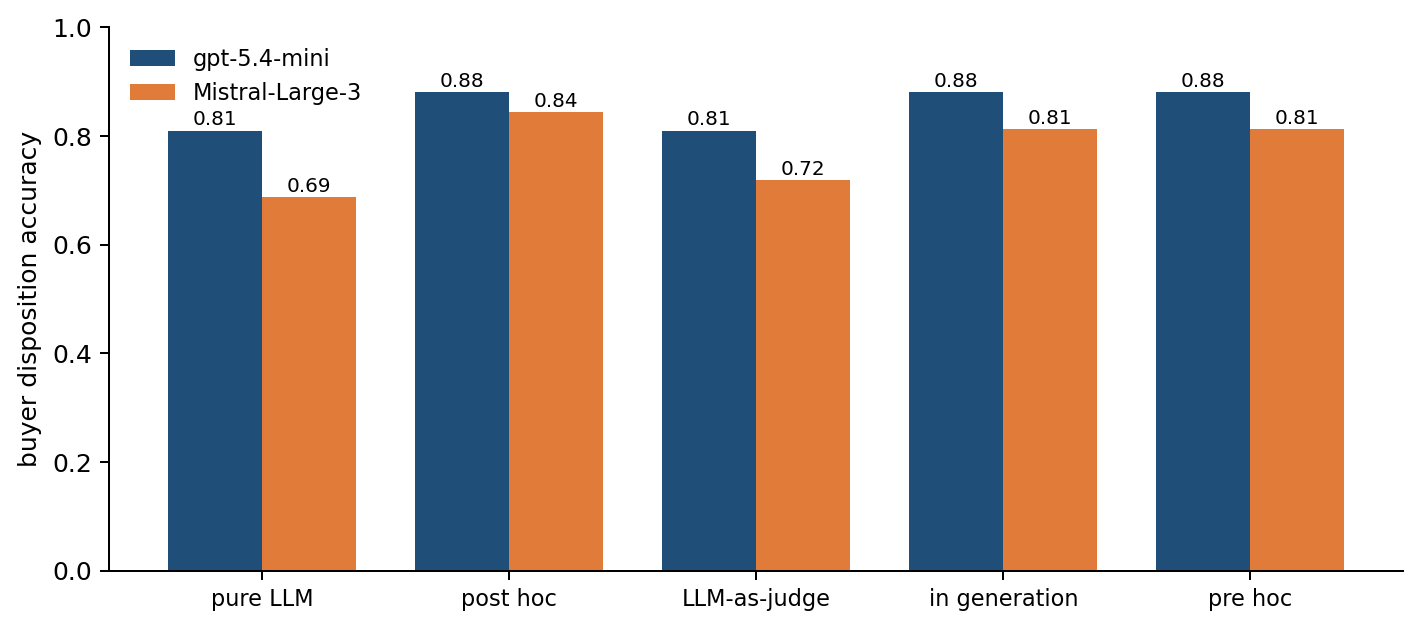
\includegraphics[width=0.82\textwidth]{Figures/fig_mistral_vs_gpt_accuracy.png}
\caption{Per-design disposition accuracy on the 32 buyer cases under the primary model (gpt-5.4-mini) and the second model (Mistral-Large-3).}
\label{fig:app:crossmodel:acc}
\end{figure}

\begin{figure}[htbp]
\centering
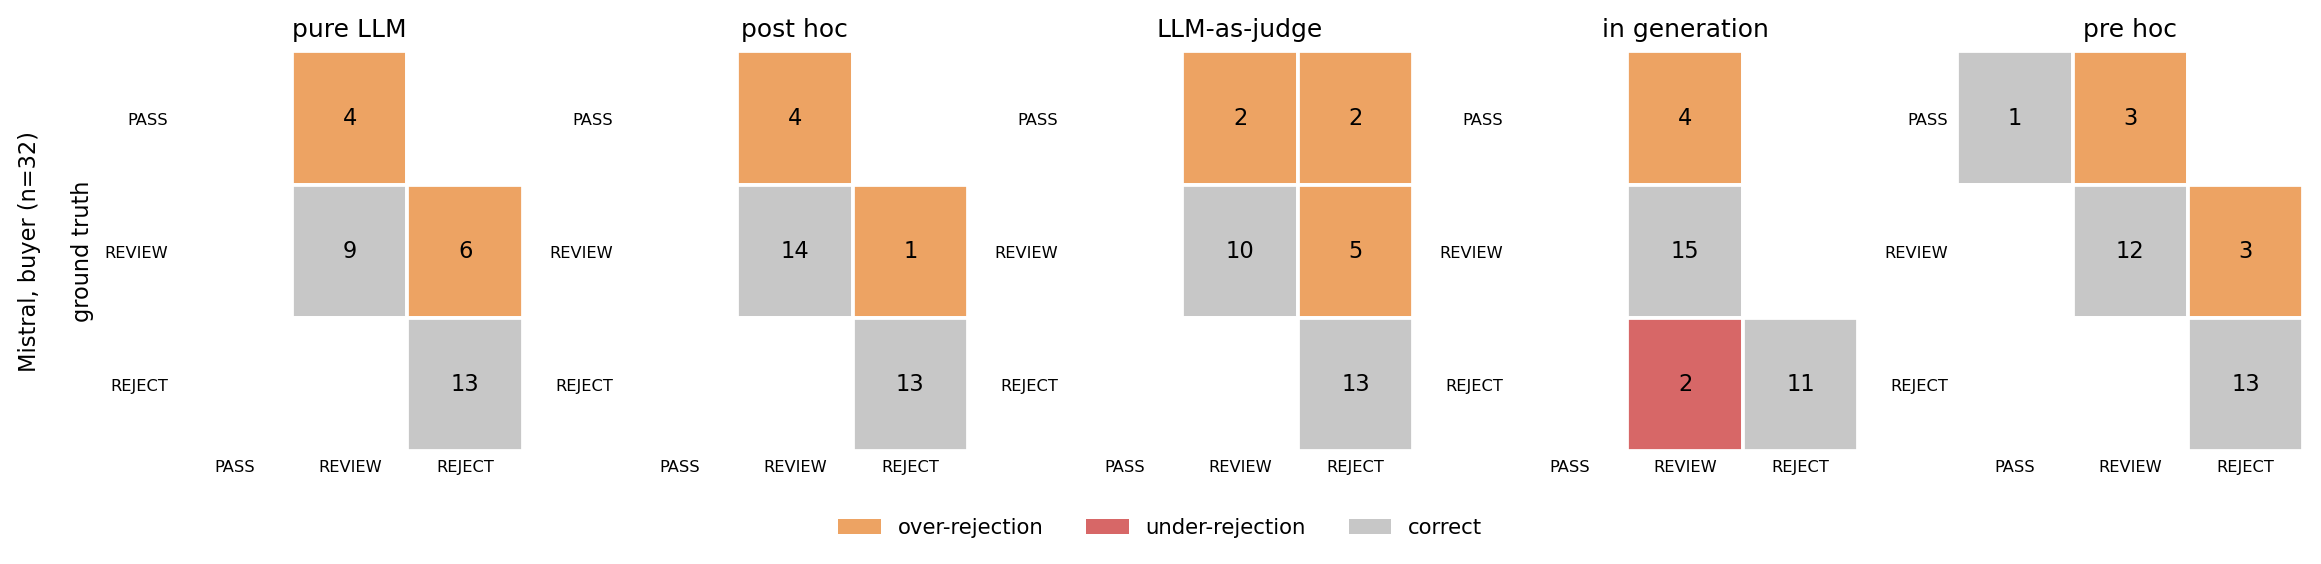
\includegraphics[width=\textwidth]{Figures/fig_mistral_confusion_buyer.png}
\caption{Disposition confusion matrices on the 32 buyer cases under Mistral-Large-3, one panel per design.}
\label{fig:app:crossmodel:conf}
\end{figure}

\begin{table}[htbp]
\centering
\caption{Error direction, reproducibility and per-run latency per design under Mistral-Large-3, buyer cohort (32 cases). Over-rejection routes a sound ASN to manual review; under-rejection lets a defective ASN through. Identical counts cases with the same disposition in all 3 replays.}
\label{tab:app:crossmodel:errors}
\footnotesize
\begin{adjustbox}{max width=\textwidth}
\begin{tabular}{@{}lcccc@{}}
\toprule
\textbf{Design} & \textbf{Over-rejections} & \textbf{Under-rejections} & \textbf{Identical across 3 replays} & \textbf{Median latency (s)} \\
\midrule
pure LLM      & 10 & 0 & 27/32 & 82.3 \\
post hoc      & 5  & 0 & 28/32 & 79.9 \\
LLM-as-judge  & 9  & 0 & 21/32 & 94.4 \\
in generation & 4  & 2 & 25/32 & 102.3 \\
pre hoc       & 6  & 0 & 26/32 & 61.1 \\
\bottomrule
\end{tabular}
\end{adjustbox}
\end{table}

Three patterns from the primary model carry over to the second. First, the safety asymmetry: the post hoc and pre hoc designs make every error in the over-rejection direction, while in generation is again the only design to under-reject, letting 2 defective ASNs through, so the soft enforcer is the first to lose the safety property as the model weakens. Second, the reproducibility order is preserved: LLM-as-judge is the least stable across replays (21/32 identical) and the enforcer-bearing designs the most stable, mirroring the primary model. Third, the operational ranking holds: pre hoc has the lowest latency (61~s median) even on this model. Latency is the one figure that shifts in absolute terms. Every design runs roughly 5 to 8 times slower than the primary model's 7.9 to 13.9~s, so the larger model buys no accuracy here and costs time. The enforcer's protective effect, its safety direction and its stability are therefore properties of the architecture and survive the model swap, while raw accuracy and speed track the model.

\paragraph{Synthetic cohort under the second model.} The second model was also run on the synthetic cohort (67 cases, majority of 3 replays), scored by construction as in Section~\ref{sec:results:synthetic}. Under the per-model tool-use accommodation 27 of the 216 in generation runs (about 12 per cent) returned transport errors; these are outvoted by the majority of 3 replays, so the design is reported on the same basis as the others. Table~\ref{tab:app:crossmodel:syn} reports disposition accuracy, single rule recall over the 41 evaluable targets, and failed PASS controls for the 5 designs.

\begin{table}[htb]
\centering
\caption{Synthetic cohort under Mistral-Large-3 (67 cases, majority of 3 replays): disposition accuracy, single rule recall over the 41 evaluable targets, and failed PASS controls (of 9 single rule clean cases).}
\label{tab:app:crossmodel:syn}
\footnotesize
\begin{tabular}{@{}lcccc@{}}
\toprule
\textbf{Design} & \textbf{Enforcer?} & \textbf{Accuracy} & \textbf{Recall} & \textbf{Failed PASS controls} \\
\midrule
pure LLM      & no  & 0.58 & 17/41 & 8/9 \\
post hoc      & yes & 0.64 & 23/41 & 7/9 \\
LLM-as-judge  & no  & 0.49 & 16/41 & 8/9 \\
in generation & yes & 0.84 & 30/41 & 2/9 \\
pre hoc       & yes & 0.69 & 24/41 & 2/9 \\
\bottomrule
\end{tabular}
\end{table}

Two findings carry over from the primary model. First, the LLM-as-judge design is again the weakest, lowest on both accuracy (0.49) and recall (16 of 41). It fails 8 of the 9 single rule PASS controls, the same over-harshness that collapses it on the primary model, so the collapse replicates across model families. The absolute spread is narrower, because the second model is a weaker fit for the task. Second, the enforcer bearing designs lead on accuracy, with in generation highest on this cohort (0.84). On specificity the picture is mixed: in generation and pre hoc fail only 2 of the 9 PASS controls, while post hoc fails 7, closer to the enforcer free designs. The per-design confusion matrices behind these numbers are shown in Figure~\ref{fig:app:crossmodel:syn:conf}, where under-rejections are more prominent than on the buyer cohort, as expected for a weaker model on the harder synthetic cases.

\begin{figure}[htb]
\centering
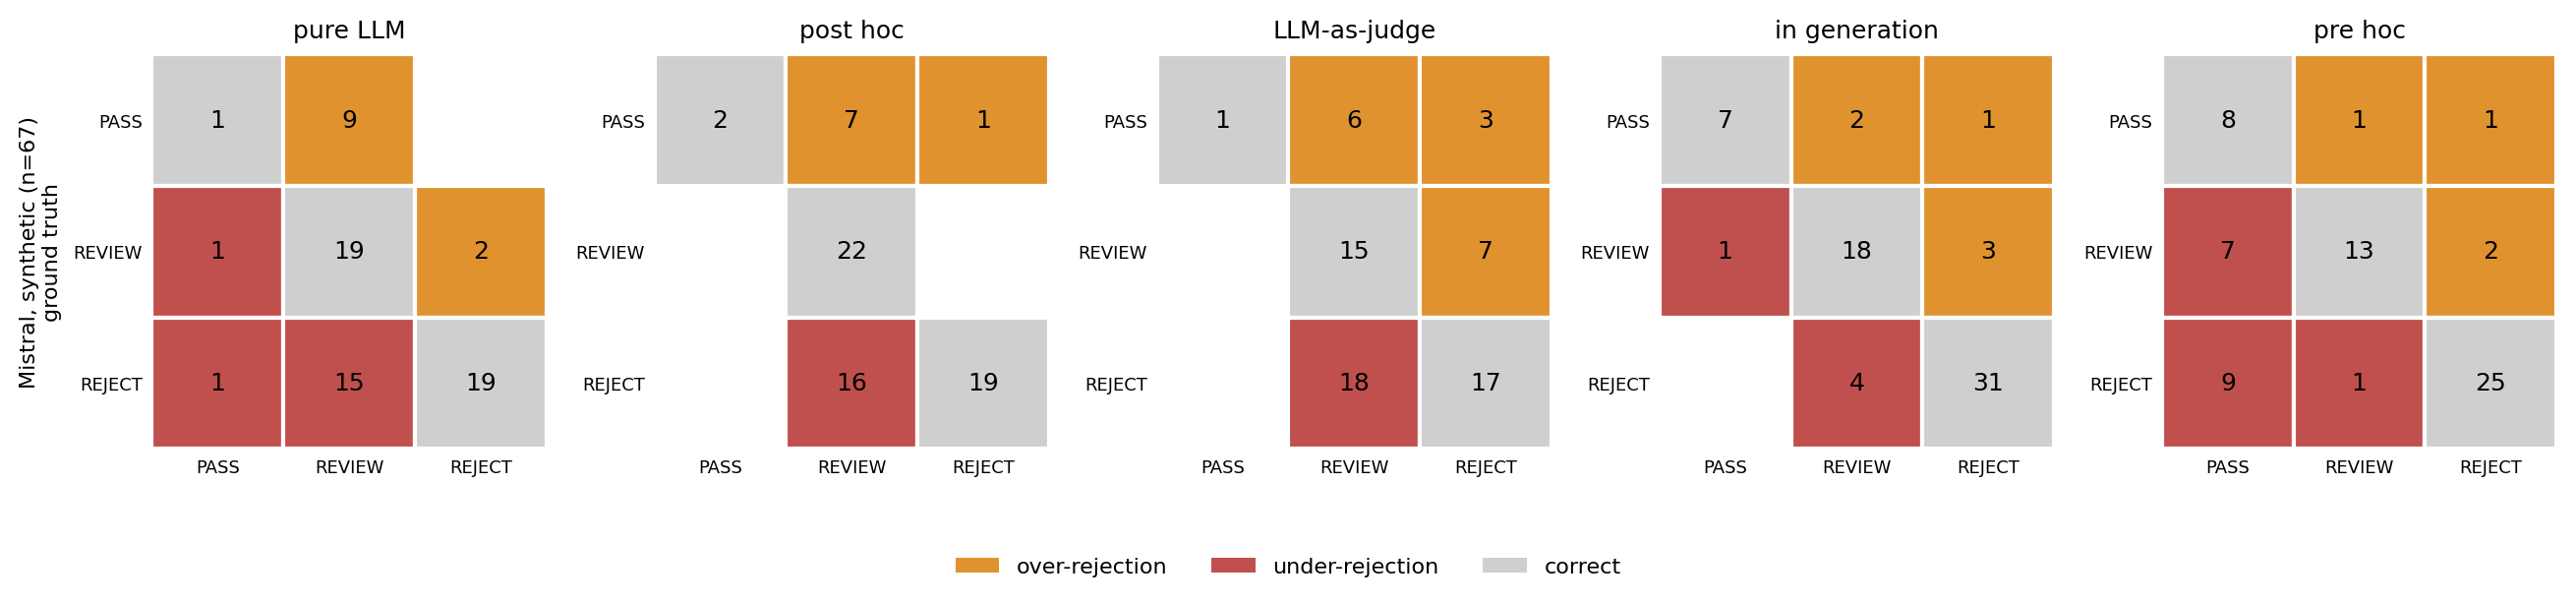
\includegraphics[width=\textwidth]{Figures/fig_mistral_confusion_synthetic.png}
\caption{Disposition confusion matrices on the 67 synthetic cases under Mistral-Large-3, one panel per design. Rows are the by-construction ground truth, columns the pipeline disposition.}
\label{fig:app:crossmodel:syn:conf}
\end{figure}

\end{singlespace}

\end{document}
